% Options for packages loaded elsewhere
\PassOptionsToPackage{unicode}{hyperref}
\PassOptionsToPackage{hyphens}{url}
\PassOptionsToPackage{dvipsnames,svgnames,x11names}{xcolor}
%
\documentclass[
  letterpaper,
  DIV=11]{scrreprt}

\usepackage{amsmath,amssymb}
\usepackage{iftex}
\ifPDFTeX
  \usepackage[T1]{fontenc}
  \usepackage[utf8]{inputenc}
  \usepackage{textcomp} % provide euro and other symbols
\else % if luatex or xetex
  \usepackage{unicode-math}
  \defaultfontfeatures{Scale=MatchLowercase}
  \defaultfontfeatures[\rmfamily]{Ligatures=TeX,Scale=1}
\fi
\usepackage{lmodern}
\ifPDFTeX\else  
    % xetex/luatex font selection
\fi
% Use upquote if available, for straight quotes in verbatim environments
\IfFileExists{upquote.sty}{\usepackage{upquote}}{}
\IfFileExists{microtype.sty}{% use microtype if available
  \usepackage[]{microtype}
  \UseMicrotypeSet[protrusion]{basicmath} % disable protrusion for tt fonts
}{}
\makeatletter
\@ifundefined{KOMAClassName}{% if non-KOMA class
  \IfFileExists{parskip.sty}{%
    \usepackage{parskip}
  }{% else
    \setlength{\parindent}{0pt}
    \setlength{\parskip}{6pt plus 2pt minus 1pt}}
}{% if KOMA class
  \KOMAoptions{parskip=half}}
\makeatother
\usepackage{xcolor}
\setlength{\emergencystretch}{3em} % prevent overfull lines
\setcounter{secnumdepth}{5}
% Make \paragraph and \subparagraph free-standing
\makeatletter
\ifx\paragraph\undefined\else
  \let\oldparagraph\paragraph
  \renewcommand{\paragraph}{
    \@ifstar
      \xxxParagraphStar
      \xxxParagraphNoStar
  }
  \newcommand{\xxxParagraphStar}[1]{\oldparagraph*{#1}\mbox{}}
  \newcommand{\xxxParagraphNoStar}[1]{\oldparagraph{#1}\mbox{}}
\fi
\ifx\subparagraph\undefined\else
  \let\oldsubparagraph\subparagraph
  \renewcommand{\subparagraph}{
    \@ifstar
      \xxxSubParagraphStar
      \xxxSubParagraphNoStar
  }
  \newcommand{\xxxSubParagraphStar}[1]{\oldsubparagraph*{#1}\mbox{}}
  \newcommand{\xxxSubParagraphNoStar}[1]{\oldsubparagraph{#1}\mbox{}}
\fi
\makeatother

\usepackage{color}
\usepackage{fancyvrb}
\newcommand{\VerbBar}{|}
\newcommand{\VERB}{\Verb[commandchars=\\\{\}]}
\DefineVerbatimEnvironment{Highlighting}{Verbatim}{commandchars=\\\{\}}
% Add ',fontsize=\small' for more characters per line
\usepackage{framed}
\definecolor{shadecolor}{RGB}{241,243,245}
\newenvironment{Shaded}{\begin{snugshade}}{\end{snugshade}}
\newcommand{\AlertTok}[1]{\textcolor[rgb]{0.68,0.00,0.00}{#1}}
\newcommand{\AnnotationTok}[1]{\textcolor[rgb]{0.37,0.37,0.37}{#1}}
\newcommand{\AttributeTok}[1]{\textcolor[rgb]{0.40,0.45,0.13}{#1}}
\newcommand{\BaseNTok}[1]{\textcolor[rgb]{0.68,0.00,0.00}{#1}}
\newcommand{\BuiltInTok}[1]{\textcolor[rgb]{0.00,0.23,0.31}{#1}}
\newcommand{\CharTok}[1]{\textcolor[rgb]{0.13,0.47,0.30}{#1}}
\newcommand{\CommentTok}[1]{\textcolor[rgb]{0.37,0.37,0.37}{#1}}
\newcommand{\CommentVarTok}[1]{\textcolor[rgb]{0.37,0.37,0.37}{\textit{#1}}}
\newcommand{\ConstantTok}[1]{\textcolor[rgb]{0.56,0.35,0.01}{#1}}
\newcommand{\ControlFlowTok}[1]{\textcolor[rgb]{0.00,0.23,0.31}{\textbf{#1}}}
\newcommand{\DataTypeTok}[1]{\textcolor[rgb]{0.68,0.00,0.00}{#1}}
\newcommand{\DecValTok}[1]{\textcolor[rgb]{0.68,0.00,0.00}{#1}}
\newcommand{\DocumentationTok}[1]{\textcolor[rgb]{0.37,0.37,0.37}{\textit{#1}}}
\newcommand{\ErrorTok}[1]{\textcolor[rgb]{0.68,0.00,0.00}{#1}}
\newcommand{\ExtensionTok}[1]{\textcolor[rgb]{0.00,0.23,0.31}{#1}}
\newcommand{\FloatTok}[1]{\textcolor[rgb]{0.68,0.00,0.00}{#1}}
\newcommand{\FunctionTok}[1]{\textcolor[rgb]{0.28,0.35,0.67}{#1}}
\newcommand{\ImportTok}[1]{\textcolor[rgb]{0.00,0.46,0.62}{#1}}
\newcommand{\InformationTok}[1]{\textcolor[rgb]{0.37,0.37,0.37}{#1}}
\newcommand{\KeywordTok}[1]{\textcolor[rgb]{0.00,0.23,0.31}{\textbf{#1}}}
\newcommand{\NormalTok}[1]{\textcolor[rgb]{0.00,0.23,0.31}{#1}}
\newcommand{\OperatorTok}[1]{\textcolor[rgb]{0.37,0.37,0.37}{#1}}
\newcommand{\OtherTok}[1]{\textcolor[rgb]{0.00,0.23,0.31}{#1}}
\newcommand{\PreprocessorTok}[1]{\textcolor[rgb]{0.68,0.00,0.00}{#1}}
\newcommand{\RegionMarkerTok}[1]{\textcolor[rgb]{0.00,0.23,0.31}{#1}}
\newcommand{\SpecialCharTok}[1]{\textcolor[rgb]{0.37,0.37,0.37}{#1}}
\newcommand{\SpecialStringTok}[1]{\textcolor[rgb]{0.13,0.47,0.30}{#1}}
\newcommand{\StringTok}[1]{\textcolor[rgb]{0.13,0.47,0.30}{#1}}
\newcommand{\VariableTok}[1]{\textcolor[rgb]{0.07,0.07,0.07}{#1}}
\newcommand{\VerbatimStringTok}[1]{\textcolor[rgb]{0.13,0.47,0.30}{#1}}
\newcommand{\WarningTok}[1]{\textcolor[rgb]{0.37,0.37,0.37}{\textit{#1}}}

\providecommand{\tightlist}{%
  \setlength{\itemsep}{0pt}\setlength{\parskip}{0pt}}\usepackage{longtable,booktabs,array}
\usepackage{calc} % for calculating minipage widths
% Correct order of tables after \paragraph or \subparagraph
\usepackage{etoolbox}
\makeatletter
\patchcmd\longtable{\par}{\if@noskipsec\mbox{}\fi\par}{}{}
\makeatother
% Allow footnotes in longtable head/foot
\IfFileExists{footnotehyper.sty}{\usepackage{footnotehyper}}{\usepackage{footnote}}
\makesavenoteenv{longtable}
\usepackage{graphicx}
\makeatletter
\def\maxwidth{\ifdim\Gin@nat@width>\linewidth\linewidth\else\Gin@nat@width\fi}
\def\maxheight{\ifdim\Gin@nat@height>\textheight\textheight\else\Gin@nat@height\fi}
\makeatother
% Scale images if necessary, so that they will not overflow the page
% margins by default, and it is still possible to overwrite the defaults
% using explicit options in \includegraphics[width, height, ...]{}
\setkeys{Gin}{width=\maxwidth,height=\maxheight,keepaspectratio}
% Set default figure placement to htbp
\makeatletter
\def\fps@figure{htbp}
\makeatother
% definitions for citeproc citations
\NewDocumentCommand\citeproctext{}{}
\NewDocumentCommand\citeproc{mm}{%
  \begingroup\def\citeproctext{#2}\cite{#1}\endgroup}
\makeatletter
 % allow citations to break across lines
 \let\@cite@ofmt\@firstofone
 % avoid brackets around text for \cite:
 \def\@biblabel#1{}
 \def\@cite#1#2{{#1\if@tempswa , #2\fi}}
\makeatother
\newlength{\cslhangindent}
\setlength{\cslhangindent}{1.5em}
\newlength{\csllabelwidth}
\setlength{\csllabelwidth}{3em}
\newenvironment{CSLReferences}[2] % #1 hanging-indent, #2 entry-spacing
 {\begin{list}{}{%
  \setlength{\itemindent}{0pt}
  \setlength{\leftmargin}{0pt}
  \setlength{\parsep}{0pt}
  % turn on hanging indent if param 1 is 1
  \ifodd #1
   \setlength{\leftmargin}{\cslhangindent}
   \setlength{\itemindent}{-1\cslhangindent}
  \fi
  % set entry spacing
  \setlength{\itemsep}{#2\baselineskip}}}
 {\end{list}}
\usepackage{calc}
\newcommand{\CSLBlock}[1]{\hfill\break\parbox[t]{\linewidth}{\strut\ignorespaces#1\strut}}
\newcommand{\CSLLeftMargin}[1]{\parbox[t]{\csllabelwidth}{\strut#1\strut}}
\newcommand{\CSLRightInline}[1]{\parbox[t]{\linewidth - \csllabelwidth}{\strut#1\strut}}
\newcommand{\CSLIndent}[1]{\hspace{\cslhangindent}#1}

% load packages
\usepackage{geometry}
\usepackage{xcolor}
\usepackage{eso-pic}
\usepackage{fancyhdr}
\usepackage{sectsty}
\usepackage{fontspec}
\usepackage{titlesec}

%% Set page size with a wider right margin
\geometry{a4paper, total={170mm,257mm}, left=20mm, top=20mm, bottom=20mm, right=50mm}

%% Let's define some colours
\definecolor{light}{HTML}{E6E6FA}
\definecolor{highlight}{HTML}{800080}
\definecolor{dark}{HTML}{330033}

%% Let's add the border on the right hand side 
\AddToShipoutPicture{% 
    \AtPageLowerLeft{% 
        \put(\LenToUnit{\dimexpr\paperwidth-3cm},0){% 
            \color{light}\rule{3cm}{\LenToUnit\paperheight}%
          }%
     }%
     % logo
    \AtPageLowerLeft{% start the bar at the bottom right of the page
        \put(\LenToUnit{\dimexpr\paperwidth-2.25cm},27.2cm){% move it to the top right
            \color{light}
\includegraphics[width=1.5cm]{_extensions/nrennie/PrettyPDF/logo.png}
          }%
     }%
}

%% Style the page number
\fancypagestyle{mystyle}{
  \fancyhf{}
  \renewcommand\headrulewidth{0pt}
  \fancyfoot[R]{\thepage}
  \fancyfootoffset{3.5cm}
}
\setlength{\footskip}{20pt}

%% style the chapter/section fonts
\chapterfont{\color{dark}\fontsize{20}{16.8}\selectfont}
\sectionfont{\color{dark}\fontsize{20}{16.8}\selectfont}
\subsectionfont{\color{dark}\fontsize{14}{16.8}\selectfont}
\titleformat{\subsection}
  {\sffamily\Large\bfseries}{\thesubsection}{1em}{}[{\titlerule[0.8pt]}]
  
\titleformat{\chapter}{\sffamily\Huge\bfseries}{\thechapter}{1em}{}[]
  
% left align title
\makeatletter
\renewcommand{\maketitle}{\bgroup\setlength{\parindent}{0pt}
\begin{flushleft}
  {\sffamily\huge\textbf{\MakeUppercase{\@title}}} \vspace{0.3cm} \newline
  {\Large {\@subtitle}} \newline
  \@author
\end{flushleft}\egroup
}
\makeatother

%% Use some custom fonts
\setsansfont{Ubuntu}[
    Path=_extensions/nrennie/PrettyPDF/Ubuntu/,
    Scale=0.9,
    Extension = .ttf,
    UprightFont=*-Regular,
    BoldFont=*-Bold,
    ItalicFont=*-Italic,
    ]

\setmainfont{Ubuntu}[
    Path=_extensions/nrennie/PrettyPDF/Ubuntu/,
    Scale=0.9,
    Extension = .ttf,
    UprightFont=*-Regular,
    BoldFont=*-Bold,
    ItalicFont=*-Italic,
    ]
    
\makeatletter
\renewenvironment{description}%
               {\list{}{\leftmargin=0pt % <------- Adjust this length
                        \labelwidth\z@ \itemindent-\leftmargin
                        \let\makelabel\descriptionlabel}}%
               {\endlist}
\makeatother
\usepackage{my_quarto_tools}
\newcommand{\cmd}[1]{\texttt{#1}\xspace}
\newcommand{\script}[1]{\texttt{#1}\xspace}
\newcommand{\key}[1]{\texttt{#1}\xspace}
\newcommand{\git}{\textit{git}\xspace}
\newcommand{\gitserver}{\textit{git}-Server\xspace}
\newcommand{\gitservers}{\textit{git}-Servers\xspace}
\newcommand{\strg}[1]{strg + #1\xspace}
\newcommand{\alt}[1]{alt + #1\xspace}
\newcommand{\datei}[1]{\textit{#1}\xspace}
\newcommand{\ordner}[1]{\textit{#1}\xspace}
\newcommand{\branch}[1]{\textit{#1}\xspace}
\newcommand{\work}{\textit{Workingdir}\xspace}
\KOMAoption{captions}{tableheading}
\makeatletter
\@ifpackageloaded{bookmark}{}{\usepackage{bookmark}}
\makeatother
\makeatletter
\@ifpackageloaded{caption}{}{\usepackage{caption}}
\AtBeginDocument{%
\ifdefined\contentsname
  \renewcommand*\contentsname{Inhaltsverzeichnis}
\else
  \newcommand\contentsname{Inhaltsverzeichnis}
\fi
\ifdefined\listfigurename
  \renewcommand*\listfigurename{Abbildungsverzeichnis}
\else
  \newcommand\listfigurename{Abbildungsverzeichnis}
\fi
\ifdefined\listtablename
  \renewcommand*\listtablename{Tabellenverzeichnis}
\else
  \newcommand\listtablename{Tabellenverzeichnis}
\fi
\ifdefined\figurename
  \renewcommand*\figurename{Abbildung}
\else
  \newcommand\figurename{Abbildung}
\fi
\ifdefined\tablename
  \renewcommand*\tablename{Tabelle}
\else
  \newcommand\tablename{Tabelle}
\fi
}
\@ifpackageloaded{float}{}{\usepackage{float}}
\floatstyle{ruled}
\@ifundefined{c@chapter}{\newfloat{codelisting}{h}{lop}}{\newfloat{codelisting}{h}{lop}[chapter]}
\floatname{codelisting}{Listing}
\newcommand*\listoflistings{\listof{codelisting}{Listingverzeichnis}}
\makeatother
\makeatletter
\makeatother
\makeatletter
\@ifpackageloaded{caption}{}{\usepackage{caption}}
\@ifpackageloaded{subcaption}{}{\usepackage{subcaption}}
\makeatother
\makeatletter
\@ifpackageloaded{tcolorbox}{}{\usepackage[skins,breakable]{tcolorbox}}
\makeatother
\makeatletter
\@ifundefined{shadecolor}{\definecolor{shadecolor}{rgb}{.97, .97, .97}}{}
\makeatother
\makeatletter
\@ifundefined{codebgcolor}{\definecolor{codebgcolor}{named}{light}}{}
\makeatother
\makeatletter
\ifdefined\Shaded\renewenvironment{Shaded}{\begin{tcolorbox}[enhanced, sharp corners, boxrule=0pt, colback={codebgcolor}, breakable, frame hidden]}{\end{tcolorbox}}\fi
\makeatother
\makeatletter
\@ifpackageloaded{tikz}{}{\usepackage{tikz}}
\makeatother
        \newcommand*\circled[1]{\tikz[baseline=(char.base)]{
          \node[shape=circle,draw,inner sep=1pt] (char) {{\scriptsize#1}};}}  
                  

\ifLuaTeX
\usepackage[bidi=basic]{babel}
\else
\usepackage[bidi=default]{babel}
\fi
\babelprovide[main,import]{ngerman}
% get rid of language-specific shorthands (see #6817):
\let\LanguageShortHands\languageshorthands
\def\languageshorthands#1{}
\ifLuaTeX
  \usepackage{selnolig}  % disable illegal ligatures
\fi
\usepackage{bookmark}

\IfFileExists{xurl.sty}{\usepackage{xurl}}{} % add URL line breaks if available
\urlstyle{same} % disable monospaced font for URLs
\hypersetup{
  pdftitle={Git Workshop},
  pdfauthor={Wolfgang Höfer},
  pdflang={de},
  colorlinks=true,
  linkcolor={highlight},
  filecolor={Maroon},
  citecolor={Blue},
  urlcolor={highlight},
  pdfcreator={LaTeX via pandoc}}


\title{Git Workshop}
\author{Wolfgang Höfer}
\date{2025-10-04}

\begin{document}
\maketitle

\pagestyle{mystyle}


\bookmarksetup{startatroot}

\chapter*{Vorbemerkung}\label{vorbemerkung}
\addcontentsline{toc}{chapter}{Vorbemerkung}

\markboth{Vorbemerkung}{Vorbemerkung}

Ein Betrieb von \git direkt auf Windows ist nicht sinnvoll. Es wird also
ein System wie MacOS oder Linux vorausgesetzt.

Dieses Handout ist in folgende Sinnabschnitte unterteilt

\begin{itemize}
\tightlist
\item
  Ein minimaler \git-Server
\item
  Grundlagen der Arbeit mit \git
\item
  Installation eines vollwertigen Gitea-Servers
\end{itemize}

\bookmarksetup{startatroot}

\chapter{Erster Überblick}\label{erster-uxfcberblick}

Eine Einführung in die Arbeit mit \git und Installation der
entsprechenden Server-Software ist etwas schwierig, weil auf einen
Schlag so viele neue Konzepte zu verarbeiten sind.

Bevor wir diese beiden Themen angehen, kann ein kleiner Überblick
hilfreich sein.

\section{Lokal -- Remote}\label{lokal-remote}

Du kannst ganz alleine auf deinem Rechner mit \git arbeiten und hast
dann deinen Arbeitsordner mit Unterstütung von \git (eigenes, lokales
Repository).

Sind an einem Projekt mehr Leute beteiligt, dann wird im Normalfall auf
einem Server ein zentrales Repository erstellt, von dem sich jeder
Mitarbeiter eine Kopie als lokales Repository auf den eigenen Rechner
holt (clont).

Der Unterschied beim Arbeiten in den beiden Varianten ist, dass die
Änderungen der lokalen Repositories immer wieder mit dem zentralen
Repository abgeglichen werden müssen (push) und dass sich die anderen
Mitarbeiter diese Änderungen auch alle holen müssen (pull).

Natürlich kann es dabei passieren, dass verschiedene Mitarbeiter die
gleiche Datei verändern und dann müssen die entstehenden Konflikte
\emph{irgendwie} behoben werden -- Hier hilft \git.

In diesen wenigen Zeilen stecken sehr viele technische Details, die wir
im Rahmen dieses Workshops auf keinen Fall alle besprechen können.

\section{Idealer Projektablauf}\label{idealer-projektablauf}

Beschränken wir uns zuerst auf den lokalen Fall und eine ideale Welt.\\
In diesem Fall würdest du keine Fehler machen, immer genau wissen was du
der Reihe nach machst -- perfekte Welt eben.

Dein Arbeitsablauf wäre dann ganz einfach:

\begin{itemize}
\tightlist
\item
  Änderung programmieren
\item
  Änderungen herrichten zum Protokollierung
\item
  Änderung festschreiben im Protokoll
\end{itemize}

In der Sprache von \git werden die letzten beiden Schritt als \emph{add}
und \emph{commit} bezeichnet.

\section{Realistischer}\label{realistischer}

Wahrscheinlich musst du ab und zu Dinge ausprobieren und willst dafür
deinen funktionierenden Code nicht gefährden.\\
In diesem Fall erstellst du einen Entwicklungszweig (branch), in dem du
in Ruhe arbeiten kannst. Wenn du mit deinem Ergebnis zufrieden bist,
dann übernimmst du deine Entwicklung -- wenn nicht, dann löschst du sie
wieder.

Man muss hier aber gleich sagen, dass das eine extreme Vereinfachung der
Realität darstellt. Mit Branches gibt es viele Varianten, die zu
besprechen wären.

\section{Im Team}\label{im-team}

Werfen wir noch einen kurzen Blick auf die Entwicklung im Team.\\
Die Wahrscheinlichkeit für das Auftreten von Konflikten ist hier
natürlich viel größer und da ist es sehr hilfreich, dass \git uns
unterstützt. Im Prinzip werden bei der Konfliktlösung -- sofern nicht
automatisch möglich -- beide (alle) Varianten in die betroffene Datei
geschrieben. Dabei wird jeweils die Herkunft angegeben und der
Zuständige für Konfliktlösung kann löschen oder übernehmen, was er für
richtig hält -- auch das ist grob vereinfacht!

\bookmarksetup{startatroot}

\chapter{Lokaler Rechner}\label{lokaler-rechner}

\section{Vorüberlegung}\label{voruxfcberlegung}

Um mit \git arbeiten zu können, brauchst du eine geeignete
Client-Software auf deinem Computer\footnote{Diese Aussage ist nur
  bedingt richtig, weil für manche Szenarien auch eine reine
  Online-Plattform genügt.}. Viele Entwicklungsumgebungen bringen ihren
individuellen \git-Client mit, was eine pauschale Behandlung erschwert.

Du solltest zuerst die typischen Abläufe direkt mit \git einüben, bevor
du dich mit grafischen Systemen beschäftigst.

\section{Installation von Git}\label{installation-von-git}

Bei der Installation von \git werden automatisch Client und Server
installiert. Du wirst hier aber nur den Client (=\git-Bash) verwenden.\\
Dabei handelt es sich um eine extrem abgespeckte Linux-Umgebung, so dass
wir auch die Grundbefehle im Terminal besprechen müssen.

Lade von \href{https://gitforwindows.org}{gitforwindows.org} die
Installationsdatei herunter, beginne aber noch nicht mit der
Installation!

Lade von
\href{https://notepad-plus-plus.org/downloads/}{notepad-plus-plus.org}
den Editor \emph{notepad++} herunter und installiere das Programm. Du
wirst bei der Installation von Git nach diesem Programm gefragt!

Starte nun die Installation von \git durch Doppelklick auf die
Installationsdatei. Die nachfolgenden Bilder zeigen den Ablauf in der
Version vom Februar 2025.

TODO: Bilder

\section{Bash Grundlagen}\label{bash-grundlagen}

Du kannst die \git-Bash aus dem Explorer heraus im gewünschten Ordner
(z.B. Projektordner) öffnen.

Jeder Befehl in der \git-Bash wird nach Drücken der \key{Enter}-Taste
ausgeführt.

\textbf{Wichtige Befehle}

\begin{longtable}[]{@{}ll@{}}
\toprule\noalign{}
Befehl & Kurzerklärung \\
\midrule\noalign{}
\endhead
\bottomrule\noalign{}
\endlastfoot
\texttt{ls\ -la} & Auflisten aller Dateien im Ordner \\
\texttt{cd} & Wechsel in den Home-Ordner \\
\texttt{cd\ \textless{}ordner\textgreater{}} & Wechsel in
\emph{Ordner} \\
\texttt{cd\ ..} & Wechsel eine Ebene nach oben \\
\texttt{echo\ \textless{}Text\textgreater{}} & Ausgabe von Text \\
\texttt{\textgreater{}\ \textless{}datei\textgreater{}} & Ausgabe in
Datei (s.u.) \\
\texttt{mkdir\ \textless{}ordner\textgreater{}} & Ordner erstellen \\
\texttt{rm\ -rf\ \textless{}ordner\textgreater{}} & Ordner ohne
Rückfrage löschen \\
\texttt{cat\ \textless{}datei\textgreater{}} & Inhalt der Datei komplett
ausgeben \\
\texttt{less\ \textless{}datei\textgreater{}} & Langsame Ausgabe, Ende
mit \texttt{q} \\
\end{longtable}

Für viele Beispiele sollst du schnell eine Datei mit minimalem Inhalt
erstellen, da es ja nur um Beispiele geht. Das kannst du im Prinzip mit
dem Editor von Windows aus machen, schneller ist aber

\begin{Shaded}
\begin{Highlighting}[]
\BuiltInTok{echo} \StringTok{"Probetext"} \OperatorTok{\textgreater{}}\NormalTok{ demodatei.txt }
\end{Highlighting}
\end{Shaded}

\bookmarksetup{startatroot}

\chapter{Hands On I}\label{hands-on-i}

Bevor du mit den Grundlagen der Bedienung von \git  beginnen kannst,
musst du einige Konfigurationsschritte ausführen.

\samplestart

\textbf{TIPP}\\
Im Terminal kannst du mit der \emph{Pfeil hoch} Taste durch die letzten
Befehle blättern -- damit gehen manche Dinge sehr schnell! \sampleend

\section{Konfigurieren von git}\label{konfigurieren-von-git}

Öffne die \git-Bash in dem Ordner, in dem du arbeiten willst. Das geht
über die rechte Maustaste im Explorer (Dateimanager).\\
Sollte dir die Schrift im Fenter zu klein sein, kannst du sie mit
\strg{+} vergrößern.

\textbf{Aktuelle Einstellungen ansehen}

\begin{Shaded}
\begin{Highlighting}[]
\CommentTok{\# Eingabe}
\FunctionTok{git}\NormalTok{ config }\AttributeTok{{-}{-}list}

\CommentTok{\# Ausgabe}
\ExtensionTok{user.email=}
\ExtensionTok{user.name=}
     \ExtensionTok{...}
\end{Highlighting}
\end{Shaded}

\textbf{Einstellungen anpassen}

\begin{Shaded}
\begin{Highlighting}[]
\CommentTok{\# eigene Phantasiedaten verwenden}
\FunctionTok{git}\NormalTok{ config }\AttributeTok{{-}{-}global}\NormalTok{ user.name }\StringTok{"Susi Sandmann"} 
\FunctionTok{git}\NormalTok{ config }\AttributeTok{{-}{-}global}\NormalTok{ user.email=susi@sandmann.de}
\end{Highlighting}
\end{Shaded}

\section{Erste Schritt}\label{erste-schritt}

Lege nun einen Arbeitsordner für dieses \emph{Hands on} an:

\begin{Shaded}
\begin{Highlighting}[]
\FunctionTok{git}\NormalTok{ init projekt }
\BuiltInTok{cd}\NormalTok{ projekt }
\end{Highlighting}
\end{Shaded}

Erstelle eine erste Datei mit dem Namen \datei{datei1.txt}.\\
Wenn du das nicht über die \git-Bash machen willst, dann achte darauf,
dass du eine reine Textdatei erstellst -- also nicht mit Word o.ä.
sondern mit einem reinen Editor wie \emph{notepad}, \emph{notepad++}
oder einer Entwicklungsumgebung.

Schneller geht das aber mit \git-Bash\footnote{Das Zeichen
  \texttt{\textgreater{}} überschreibt alle Inhalte einer Datei,
  \texttt{\textgreater{}\textgreater{}} hängt die Daten hinten an.}.

\begin{Shaded}
\begin{Highlighting}[]
\BuiltInTok{echo} \StringTok{"Version 1"} \OperatorTok{\textgreater{}}\NormalTok{ datei1.txt }
\end{Highlighting}
\end{Shaded}

Diese Datei nimmst du dann in die Versionsverwaltung auf

\begin{Shaded}
\begin{Highlighting}[]
\FunctionTok{git}\NormalTok{ add datei1.txt }
\end{Highlighting}
\end{Shaded}

Im Anschluss erstellst du einen Commit um den aktuellen Stand deines
\emph{Projekts} festzuschreiben.

\begin{Shaded}
\begin{Highlighting}[]
\FunctionTok{git}\NormalTok{ commit }\AttributeTok{{-}m} \StringTok{"Erste Datei erstellt"}
\end{Highlighting}
\end{Shaded}

Diesen Zyklus aus \emph{add} und \emph{commit} führst du immer wieder
aus, sobald du an eine wichtige Stelle im Projektverlauf kommst.
Generell gilt: „Lieber mehr Commits, als zu wenige!{}``

Ein Commit ist ein Projektstand, an den du zurückkehren kannst, wenn
etwas grob missglückt ist. Vergeht zu viel Zeit (=viel Code) zwischen
zwei Commits, so entstehen eventuell größere Verluste bei einem
Rücksprung zum alten Stand.\\
Später im Workshop lernst du auch, wie du Commits nachträglich
zusammenfassen kannst (=squash) um deine Entwicklungsschritte
übersichtlich zu halten.

Nun änderst du deine Datei ab, indem du eine Zeile ergänzt:

\begin{Shaded}
\begin{Highlighting}[]
\BuiltInTok{echo} \StringTok{"Version 2"} \OperatorTok{\textgreater{}\textgreater{}}\NormalTok{ datei1.txt }
\FunctionTok{git}\NormalTok{ add datei1.txt }
\FunctionTok{git}\NormalTok{ commit }\AttributeTok{{-}m} \StringTok{"Erläuterung"}
\end{Highlighting}
\end{Shaded}

Du kannst gleichzeitig auch mehrere Dateien in die Versionierung
aufnehmen.

\begin{Shaded}
\begin{Highlighting}[]
\CommentTok{\# Aktuell passiert nichts {-} du hast ja nichts geändert!}
\FunctionTok{git}\NormalTok{ add . }\AttributeTok{{-}{-}all} 
\end{Highlighting}
\end{Shaded}

\samplestart

\textbf{TIPP}\\
Das \emph{adden} ist generell unabhängig vom \emph{commit}. Es ist sogar
üblich, immer erst einige Dateien anzusammeln, bevor du einen Commit
machst.\\
Es ist auch völlig unproblematisch eine Datei zwischen zwei Commits
mehrfach in der aktuellen Version mit \emph{add} für den Commit zu
registrieren.

In machen Projekte solltest du von \emph{--all} Abstand nehmen.
Vielleicht gibt es Dateien, die du absichtlich \emph{nicht} in der
Versionierung haben willst. Das ist oft bei Dateien mit Kennwörtern der
Fall. Wenn du sie in eine Datei \datei{.gitignore} einträgst, werden sie
automatisch ignoriert. \sampleend

Mit diesen Befehlen ist bereits ein einfacher lokaler
Entwicklungsprozess abbildbar. Allerdings gibt es noch viele weitere
Feinheiten und Varianten, zum Beispiel um eventuelle Fehler zu beheben.

\section{Ein genauerer Blick}\label{ein-genauerer-blick}

Der Ordner eines Projekts wird von \git in drei \emph{logische} Bereiche
unterteilt:

\begin{itemize}
\tightlist
\item
  Working-Directory (Arbeitsordner)
\item
  Stage (auch Index oder Cache genannt)
\item
  Repository
\end{itemize}

Leider werden die Begriffe nicht einheitlich verwendet und haben in
unterschiedlichem Kontext auch noch abweichende Bedeutung -- das
betrifft uns hier aber nicht. Sollte eine Möglichkeit zur Verwechslung
existieren, weise ich dich ausdrücklich darauf hin.

Mit der \emph{logischen} Unterteilung ist gemeint, dass die
unterschiedlichen Versionen der Dateien in einem speziellen Ordner
innerhalb des Projektordners verwaltet werden. Der Ordner trägt den
Namen \texttt{.git} und wird vom System ausgeblendet. Dieser Ordner
bildet den \emph{Stage} und das \emph{Repository}. Allerdings bedeutet
\emph{logisch} auch, dass diese beiden Bereiche von \git verwaltet
werden und vom unbedarften Benutzer nicht einfach unterschieden werden
können.

Betrachten wir einen Entwicklungszyklus im Detail.

Den aktuellen Stand des Projekts kannst du mit folgendem Befehl
abfragen:

\begin{Shaded}
\begin{Highlighting}[]
\CommentTok{\# Eingabe}
\FunctionTok{git}\NormalTok{ status}

\CommentTok{\# Ausgabe (Zeilenumbrüche geändert)}
\ExtensionTok{Auf}\NormalTok{ Branch master}
\ExtensionTok{nichts}\NormalTok{ zu committen, }
\ExtensionTok{Arbeitsverzeichnis}\NormalTok{ unverändert}
\end{Highlighting}
\end{Shaded}

Das bedeutet, dass du aktuelle einen \emph{sauberen} Zustand deines
Arbeitsordners ohne Änderungen hast.

Erstelle eine neue \datei{datei2.txt} und füge die Zeile \emph{Version
1} ein. In der Datei \datei{datei1.txt} kommt die Zeile \emph{Version 3}
dazu.

\begin{Shaded}
\begin{Highlighting}[]
\CommentTok{\# Eingabe (Lasse ich zukünftig weg)}
\BuiltInTok{echo} \StringTok{"Version 3"} \OperatorTok{\textgreater{}\textgreater{}}\NormalTok{ datei1.txt}
\BuiltInTok{echo} \StringTok{"Version 1"} \OperatorTok{\textgreater{}\textgreater{}}\NormalTok{ datei2.txt}
\FunctionTok{git}\NormalTok{ status }

\CommentTok{\# Ausgabe}
\ExtensionTok{Auf}\NormalTok{ Branch master}
\ExtensionTok{Änderungen,}\NormalTok{ die nicht zum Commit vorgemerkt sind:  }
  \KeywordTok{(}\ExtensionTok{benutzen}\NormalTok{ Sie }\StringTok{"git add \textless{}Datei\textgreater{}..."}\NormalTok{,  }
   \ExtensionTok{um}\NormalTok{ die Änderungen zum Commit vorzumerken}\KeywordTok{)}
  
  \KeywordTok{(}\ExtensionTok{benutzen}\NormalTok{ Sie }\StringTok{"git restore \textless{}Datei\textgreater{}..."}\NormalTok{,  }
   \ExtensionTok{um}\NormalTok{ die Änderungen im Arbeitsverzeichnis zu verwerfen}\KeywordTok{)}  

    \ExtensionTok{geändert:}\NormalTok{       datei1.txt}

\ExtensionTok{Unversionierte}\NormalTok{ Dateien:}
  \KeywordTok{(}\ExtensionTok{benutzen}\NormalTok{ Sie }\StringTok{"git add \textless{}Datei\textgreater{}..."}\NormalTok{, }
   \ExtensionTok{um}\NormalTok{ die Änderungen zum Commit vorzumerken}\KeywordTok{)}

    \ExtensionTok{datei2.txt}

\ExtensionTok{keine}\NormalTok{ Änderungen zum Commit vorgemerkt }
\KeywordTok{(}\ExtensionTok{benutzen}\NormalTok{ Sie }\StringTok{"git add"}\NormalTok{ und/oder }\StringTok{"git commit {-}a"}\KeywordTok{)}
\end{Highlighting}
\end{Shaded}

Es wird dir angezeigt, dass Änderungen im \work vorliegen.\\
Du siehst auch, dass \git die \datei{datei1.txt} bereits kennt
(=geändert) und dass \datei{datei2.txt} noch nicht in die\\
Versionsverwaltung aufgenommen wurde (=Unversioniert).

Nun werden die aktuelle Stände \emph{auf den Stage}/\emph{in den Stage}
übertragen:

\begin{Shaded}
\begin{Highlighting}[]
\FunctionTok{git}\NormalTok{ add . }\AttributeTok{{-}{-}all} 
\FunctionTok{git}\NormalTok{ status }

\CommentTok{\# Ausgabe  }
\ExtensionTok{Auf}\NormalTok{ Branch master}
\ExtensionTok{Zum}\NormalTok{ Commit vorgemerkte Änderungen:}
  \KeywordTok{(}\ExtensionTok{benutzen}\NormalTok{ Sie }\StringTok{"git restore {-}{-}staged \textless{}Datei\textgreater{}..."}  
   \ExtensionTok{zum}\NormalTok{ Entfernen aus der Staging{-}Area}\KeywordTok{)}  

    \ExtensionTok{geändert:}\NormalTok{       datei1.txt}
    \ExtensionTok{neue}\NormalTok{ Datei:     datei3.txt}
\end{Highlighting}
\end{Shaded}

Diese Dateien sind zum Commit vorgemerkt, also zum festen Eintrag in die
Projekthistorie. Der Status zeigt aktuell den \emph{Stage} an.

Als Demonstration fügen wir beiden Dateien eine weitere Zeile hinzu und
fragen wieder den Staus ab:

\begin{Shaded}
\begin{Highlighting}[]
\BuiltInTok{echo} \StringTok{"Weitere Zeile"} \OperatorTok{\textgreater{}\textgreater{}}\NormalTok{ datei1.txt  }
\BuiltInTok{echo} \StringTok{"Weitere Zeile"} \OperatorTok{\textgreater{}\textgreater{}}\NormalTok{ datei2.txt }
\FunctionTok{git}\NormalTok{ status }

\CommentTok{\# Ausgabe ( {-}{-}{-}{-} Anmerkung {-}{-}{-}{-})}
\ExtensionTok{Auf}\NormalTok{ Branch master}
\ExtensionTok{Zum}\NormalTok{ Commit vorgemerkte Änderungen:}
  \KeywordTok{(}\ExtensionTok{benutzen}\NormalTok{ Sie }\StringTok{"git restore {-}{-}staged \textless{}Datei\textgreater{}..."}  
   \ExtensionTok{zum}\NormalTok{ Entfernen aus der Staging{-}Area}\KeywordTok{)}
    
    \ExtensionTok{geändert:}\NormalTok{       datei1.txt}
    \ExtensionTok{neue}\NormalTok{ Datei:     datei2.txt}

\ExtensionTok{{-}{-}{-}{-}{-}{-}{-}{-}{-}{-}{-}{-}{-}{-}{-}}\NormalTok{ Ende Stage }\AttributeTok{{-}{-}{-}{-}{-}{-}{-}{-}{-}{-}{-}{-}}
\ExtensionTok{{-}{-}{-}{-}{-}{-}{-}{-}{-}{-}{-}{-}{-}{-}{-}}\NormalTok{ Anfang Workdir }\AttributeTok{{-}{-}{-}{-}{-}{-}{-}{-}}

\ExtensionTok{Änderungen,}\NormalTok{ die nicht zum Commit vorgemerkt sind:}
  \KeywordTok{(}\ExtensionTok{benutzen}\NormalTok{ Sie }\StringTok{"git add \textless{}Datei\textgreater{}..."}\NormalTok{, um die Änderungen }
   \ExtensionTok{zum}\NormalTok{ Commit vorzumerken}\KeywordTok{)}
  
  \KeywordTok{(}\ExtensionTok{benutzen}\NormalTok{ Sie }\StringTok{"git restore \textless{}Datei\textgreater{}..."}\NormalTok{, }
   \ExtensionTok{um}\NormalTok{ die Änderungen im Arbeitsverzeichnis zu verwerfen}\KeywordTok{)}

    \ExtensionTok{geändert:}\NormalTok{       datei1.txt}
    \ExtensionTok{geändert:}\NormalTok{       datei2.txt}
\end{Highlighting}
\end{Shaded}

Beide Dateien liegen also in verschiedenen Versionen im Stage und im
\work vor.\\
Ein Commit transferiert die Dateien aus dem Stage ins Repository, also
in die Projekthistorie.

\samplestart

\textbf{Hinweis}\\
Wenn ich hier von \emph{transferieren} spreche, so führt das zu einer
falschen Vorstellung. In Wirklichkeit werden im \emph{.git}-Ordner nur
einige Verweise geändert -- wobei das auch wieder nicht die ganze
Wahrheit ist! \sampleend

\subsection{Etwas mehr Wahrheit}\label{etwas-mehr-wahrheit}

Dieser Abschnitt ist nur ein Einblick für Interessierte. Angenommen, du
erstellst ein neues Repository

\begin{Shaded}
\begin{Highlighting}[]
\FunctionTok{git}\NormalTok{ init demo }
\BuiltInTok{cd}\NormalTok{ demo}

\BuiltInTok{echo} \StringTok{"Etwas HTML"} \OperatorTok{\textgreater{}\textgreater{}}\NormalTok{ homepage.html}
\end{Highlighting}
\end{Shaded}

Wenn du nun die Verzeichnisstruktur des Ordners \emph{.git} genauer
untersuchst, wirst du in etwa dies hier sehen:

\begin{Shaded}
\begin{Highlighting}[]
\ExtensionTok{.git/}
\ExtensionTok{├──}\NormalTok{ branches}
\ExtensionTok{├──}\NormalTok{ config}
\ExtensionTok{├──}\NormalTok{ description}
\ExtensionTok{├──}\NormalTok{ HEAD}
\ExtensionTok{├──}\NormalTok{ hooks}
\ExtensionTok{│  }\NormalTok{ ├── applypatch{-}msg.sample}
\ExtensionTok{│  }\NormalTok{ ├── commit{-}msg.sample}
\ExtensionTok{│  }\NormalTok{ ├── fsmonitor{-}watchman.sample}
\ExtensionTok{│  }\NormalTok{ ├── post{-}update.sample}
\ExtensionTok{│  }\NormalTok{ ├── pre{-}applypatch.sample}
\ExtensionTok{│  }\NormalTok{ ├── pre{-}commit.sample}
\ExtensionTok{│  }\NormalTok{ ├── pre{-}merge{-}commit.sample}
\ExtensionTok{│  }\NormalTok{ ├── prepare{-}commit{-}msg.sample}
\ExtensionTok{│  }\NormalTok{ ├── pre{-}push.sample}
\ExtensionTok{│  }\NormalTok{ ├── pre{-}rebase.sample}
\ExtensionTok{│  }\NormalTok{ ├── pre{-}receive.sample}
\ExtensionTok{│  }\NormalTok{ └── update.sample}
\ExtensionTok{├──}\NormalTok{ info}
\ExtensionTok{│  }\NormalTok{ └── exclude}
\ExtensionTok{├──}\NormalTok{ objects}
\ExtensionTok{│  }\NormalTok{ ├── info}
\ExtensionTok{│  }\NormalTok{ └── pack}
\ExtensionTok{└──}\NormalTok{ refs}
    \ExtensionTok{├──}\NormalTok{ heads}
    \ExtensionTok{└──}\NormalTok{ tags}
\end{Highlighting}
\end{Shaded}

\datei{homepage.htm}\footnote{Der Name wurde gewählt um keine
  Verwechslung zwischen index.html und dem Index von \git zu
  provozieren!} ist noch nicht versioniert, also stellt obige
Ordnerstruktur ein leeres Repository dar. Sobald du die Datei zum Commit
vormerkst

\begin{Shaded}
\begin{Highlighting}[]
\FunctionTok{git}\NormalTok{ add index.html }
\end{Highlighting}
\end{Shaded}

ändert sich im Ordner \emph{.git} etwas. Ich gebe nur die relevante
Stelle an:

\begin{Shaded}
\begin{Highlighting}[]
\ExtensionTok{├──}\NormalTok{ index            }\OperatorTok{\textless{}\textless{}\textless{}}\NormalTok{ neu }
\ExtensionTok{├──}\NormalTok{ info}
\ExtensionTok{│  }\NormalTok{ └── exclude}
\ExtensionTok{├──}\NormalTok{ objects}
\ExtensionTok{│  }\NormalTok{ ├── ce          }\OperatorTok{\textless{}\textless{}\textless{}}\NormalTok{ neu, bei dir anders! }
\ExtensionTok{│  }\NormalTok{ │   └── 1332fcf1795166c3c5cd0216b5e7dc2dce7998}
\ExtensionTok{│  }\NormalTok{ ├── info}
\ExtensionTok{│  }\NormalTok{ └── pack}
\end{Highlighting}
\end{Shaded}

Die Datei \emph{index} stellt den Stage dar. Diese Datei kannst du nicht
direkt lesen. Das geht nur mit

\begin{Shaded}
\begin{Highlighting}[]
\FunctionTok{git}\NormalTok{ ls{-}files }\AttributeTok{{-}{-}stage} 
\end{Highlighting}
\end{Shaded}

Den Hash aus dieser Ausgabe findet du oben in der Ordnerstruktur wieder.

\begin{Shaded}
\begin{Highlighting}[]
\ExtensionTok{100644}\NormalTok{ ce1332fcf1795166c3c5cd0216b5e7dc2dce7998 0   homepage.htm}
\end{Highlighting}
\end{Shaded}

Allerdings wird mit den ersten beiden Zeichen ein Ordner erstellt und in
diesem Ordner eine Datei, deren Name aus den restlichen Zeichen besteht.
Zusätzlich findet man den Dateityp (100644), den Status (Das ist
komplexer! Hier 0) und den Dateinamen.

Den Hash kannst du dir auch so anzeigen lassen:

\begin{Shaded}
\begin{Highlighting}[]
\FunctionTok{git}\NormalTok{ hash{-}object homepage.htm }
\end{Highlighting}
\end{Shaded}

Aber gehen wir einen Schritt weiter und committen die Datei:

\begin{Shaded}
\begin{Highlighting}[]
\FunctionTok{git}\NormalTok{ commit }\AttributeTok{{-}m} \StringTok{"about.html added"}
\end{Highlighting}
\end{Shaded}

Nun sieht die Ordnerstruktur verändert aus -- die Hooks habe ich in der
Darstellung aus Platzgründen entfernt!

\begin{Shaded}
\begin{Highlighting}[]
\ExtensionTok{.git/}
\ExtensionTok{├──}\NormalTok{ branches}
\ExtensionTok{├──}\NormalTok{ COMMIT\_EDITMSG}
\ExtensionTok{├──}\NormalTok{ config}
\ExtensionTok{├──}\NormalTok{ description}
\ExtensionTok{├──}\NormalTok{ HEAD}
\ExtensionTok{├──}\NormalTok{ hooks}
    \ExtensionTok{....}
\ExtensionTok{├──}\NormalTok{ index}
\ExtensionTok{├──}\NormalTok{ info}
\ExtensionTok{│  }\NormalTok{ └── exclude}
\ExtensionTok{├──}\NormalTok{ logs}
\ExtensionTok{│  }\NormalTok{ ├── HEAD}
\ExtensionTok{│  }\NormalTok{ └── refs}
\ExtensionTok{│  }\NormalTok{     └── heads}
\ExtensionTok{│  }\NormalTok{         └── master}
\ExtensionTok{├──}\NormalTok{ objects}
\ExtensionTok{│  }\NormalTok{ ├── 3b  }
\ExtensionTok{│  }\NormalTok{ │   └── 028e4d0230fb8f3553f0f7579e68e6c4e27d3f}
\ExtensionTok{│  }\NormalTok{ ├── 94}
\ExtensionTok{│  }\NormalTok{ │   └── eed25c4ef6cfa1384df66f28308c09dc9bf28d}
\ExtensionTok{│  }\NormalTok{ ├── ce}
\ExtensionTok{│  }\NormalTok{ │   └── 1332fcf1795166c3c5cd0216b5e7dc2dce7998}
\ExtensionTok{│  }\NormalTok{ ├── info}
\ExtensionTok{│  }\NormalTok{ └── pack}
\ExtensionTok{└──}\NormalTok{ refs}
    \ExtensionTok{├──}\NormalTok{ heads}
    \ExtensionTok{│  }\NormalTok{ └── master}
    \ExtensionTok{└──}\NormalTok{ tags}
\end{Highlighting}
\end{Shaded}

Wir konzentrieren uns auf die \emph{objects} und das \emph{log}.

Mit \texttt{git\ log\ -\/-oneline} erfährst du etwas über den erfolgten
Commit -- zum Beispiel seinen Hash:

\begin{Shaded}
\begin{Highlighting}[]
\ExtensionTok{commit}\NormalTok{ 3b028e4d0230fb8f3553f0f7579e68e6c4e27d3f }\ErrorTok{(}\ExtensionTok{HEAD} \AttributeTok{{-}}\OperatorTok{\textgreater{}}\NormalTok{ master}\KeywordTok{)}
\ExtensionTok{Author:}\NormalTok{ wolfgang }\OperatorTok{\textless{}}\NormalTok{hoeferwolf@t{-}online.de}\OperatorTok{\textgreater{}}
\ExtensionTok{Date:}\NormalTok{   Sun Jan 26 20:20:10 2025 +0100}

    \ExtensionTok{homepage.html}\NormalTok{ added}
\end{Highlighting}
\end{Shaded}

Durch
\texttt{git\ cat-file\ -t\ 3b028e4d0230fb8f3553f0f7579e68e6c4e27d3f}\\
siehst du, dass es wirklich ein Commit ist (unnötig),\\
durch
\texttt{git\ cat-file\ -p\ 3b028e4d0230fb8f3553f0f7579e68e6c4e27d3f}\\
gibt es weitere Details:

\begin{Shaded}
\begin{Highlighting}[]
\ExtensionTok{tree}\NormalTok{ 94eed25c4ef6cfa1384df66f28308c09dc9bf28d   }\OperatorTok{\textless{}\textless{} wichtig!}
\StringTok{author wolfgang \textless{}hoeferwolf@t{-}online.de\textgreater{} 1737919210 +0100}
\StringTok{committer wolfgang \textless{}hoeferwolf@t{-}online.de\textgreater{} 1737919210 +0100}

\StringTok{homepage.html added}
\end{Highlighting}
\end{Shaded}

Am Commit hängt also der \emph{tree} der betroffenen Dateien:

\begin{Shaded}
\begin{Highlighting}[]
\FunctionTok{git}\NormalTok{ cat{-}file }\AttributeTok{{-}p}\NormalTok{ 94eed25c4ef6cfa1384df66f28308c09dc9bf28d}
\end{Highlighting}
\end{Shaded}

Diese Ausgabe kennst du bereits aus dem Stage:

\begin{Shaded}
\begin{Highlighting}[]
\ExtensionTok{100644}\NormalTok{ blob ce1332fcf1795166c3c5cd0216b5e7dc2dce7998    homepage.html}
\end{Highlighting}
\end{Shaded}

und mit

\begin{Shaded}
\begin{Highlighting}[]
\FunctionTok{git}\NormalTok{ cat{-}file }\AttributeTok{{-}p}\NormalTok{ ce1332fcf1795166c3c5cd0216b5e7dc2dce7998}
\end{Highlighting}
\end{Shaded}

bekommst du den Inhalt der Datei:

\begin{Shaded}
\begin{Highlighting}[]
\ExtensionTok{Etwas}\NormalTok{ HTML}
\end{Highlighting}
\end{Shaded}

Du bist jetzt über mehrere Stufen zum Inhalt der Datei gelangt. Eine
kleine Stufe haben wir aber ausgelassen:

\begin{Shaded}
\begin{Highlighting}[]
\FunctionTok{git}\NormalTok{ cat{-}file }\AttributeTok{{-}t}\NormalTok{ ce1332fcf1795166c3c5cd0216b5e7dc2dce7998}
\end{Highlighting}
\end{Shaded}

liefert die Information \texttt{blob} (Binary large object). Es gibt
einen Grund, warum ich dir diesen Umweg zumute! Di siehst hier ein
grundlegendes Konzept von \git, das beim Verständnis hilft:

Der Commit zeigt auf einen Tree und im Tree stehen Dateinamen mit den
Hashes.\\
Das sind nur die Namen und nicht die Dateien! Hinter dem Hash verbirgt
sich ein \emph{blob}, also reine \emph{Roh}daten \textbf{ohne}
Dateinamen. Git verwendet das, um von verschiedenen Stellen aus auf die
gleichen Rohdaten zu verweisen. Ändern sich Dateien zwischen zwei
Commits nicht (Hash bleibt gleich), so werden sie nicht neu gespeichert.
Der neue Commit zeigt auf einen neuen Tree in dem wieder die gleichen
Hashes mit den gleichen Dateinamen stehen.

Tiefer will ich an dieser Stelle in dieses Thema nicht einsteigen!

\section{Fehlerbehebung}\label{fehlerbehebung}

Ein Versionsverwaltungsprogramm hat unter anderem die Aufgabe, ein
Projekt in gewissem Umfang revisionssicher zu protokollieren. Aus diesem
Grund müssen bestimmte \emph{Fehler} in der History erhalten bleiben.\\
Bei anderen Fehlern ist es aber wichtig, dass sie schnell und einfach
rückgängig gemacht werden können.

Relativ unproblematisch sind \emph{Reparaturen} bei lokaler Arbeit,
bevor ein Commit erfolgt ist:

\begin{itemize}
\tightlist
\item
  Neue, fehlerhafte Dateien kann man einfach löschen.
\item
  Bereits versionierte Dateien mit Fehlern können durch
  \texttt{git\ restore\ \textless{}dateiname\textgreater{}} wieder mit
  der Version aus dem Stage überschrieben werden\footnote{Es gibt auch
    noch den Befehl
    \texttt{git\ restore\ \textless{}dateiname\textgreater{}\ -\/-staged},
    der das \work unangetastet lässt und nur die Version aus dem Stage
    löscht.}
\end{itemize}

\samplestart

Vorher habe ich geschrieben, dass bei einem Commit die Dateien aus dem
Stage in die Projekthistorie übertragen und aus dem Stage entfernt
werden. Das stimmt so nicht ganz.

In Wirklichkeit zeigt \texttt{git\ status} diese Dateien nur nicht mehr
an, was auf einen leeren Stage schließen lassen würde. \sampleend

Wäre der Stage wirklich leer, so könnte nachfolgende Reparatur nicht
funktionieren -- was sie aber tut:

\begin{Shaded}
\begin{Highlighting}[]
\BuiltInTok{echo} \StringTok{"text"} \OperatorTok{\textgreater{}}\NormalTok{ datei.txt }
\FunctionTok{git}\NormalTok{ add datei.txt     }\CommentTok{\# danach im Stage }
\FunctionTok{git}\NormalTok{ commit }\AttributeTok{{-}m} \StringTok{"gesichert"}

\FunctionTok{git}\NormalTok{ status   }\CommentTok{\# Stage anscheinend leer }

\BuiltInTok{echo} \StringTok{"falscher Text"} \OperatorTok{\textgreater{}\textgreater{}}\NormalTok{ datei.txt   }\CommentTok{\#  Fehler }
\FunctionTok{git}\NormalTok{ restore datei.txt              }\CommentTok{\# repariert}
\end{Highlighting}
\end{Shaded}

\samplestart

\textbf{Hinweis}\\
Im Netz findet man oft die Variante mit \texttt{checkout}, die früher
üblich war. \texttt{restore} wurde eingeführt um eindeutigere Befehle zu
schaffen. \sampleend

Mit dem \texttt{restore}-Befehl kann man auch eine Datei aus einem
beliebigen Commit restaurieren:

\begin{Shaded}
\begin{Highlighting}[]
\FunctionTok{git}\NormalTok{ restore }\AttributeTok{{-}{-}source}\OperatorTok{=\textless{}}\NormalTok{HASH}\OperatorTok{\textgreater{}} \OperatorTok{\textless{}}\NormalTok{datei}\OperatorTok{\textgreater{}}
\end{Highlighting}
\end{Shaded}

Die Fehlerbehebung kann auch das Löschen ganzer Entwicklungs- oder
Testzweige bedeutet, was später noch besprochen wird.

\bookmarksetup{startatroot}

\chapter{Hands on II}\label{hands-on-ii}

Du wirst in diesem Abschnitt einige Dinge als redundant empfinden, weil
sie auch bereits im ersten \emph{Hands On} bereits verwendet wurden.
Sieh es einfach als Übung und da du dieses PDF ohnehin nicht ausdrucken
wirst, ist die minimal erhöhte Seitenzahl auch kein Problem.

Dieses Szenario ist etwas komplexer, da wir mit mehreren Dateien
arbeiten und auch parallele Ideen verfolgen wollen (branching).\\
Da Programmieren zu lange dauert, erstellen wir in diesem Projekt ein
kleines Buches mit Kurzgeschichten. Die Geschichten wurden von einer KI
generiert um den Arbeitsaufwand zu minimieren.

Die Einzelteile der Geschichten befinden sich in einem \git-Repository
und müssen zunächst auf den lokalen Computer geclont werden. Das ist ein
notwendiger Vorgriff auf den Abschnitt der Teamarbeit, den du hier
einfach mal ausführst. Es handelt sich um ein öffentliches Repository,
auf das auch ohne Benutzerkennung zugegriffen werden darf -- aber eben
nur lesend. Aus diesem Grund wird zum Clonen auch \emph{https} und nicht
\emph{ssh} verwendet. Öffne die \git-Bash (oder ein Terminal) und gib
ein:

\begin{Shaded}
\begin{Highlighting}[]
\FunctionTok{mkdir}\NormalTok{ fortbildung}
\BuiltInTok{cd}\NormalTok{ fortbildung}
\FunctionTok{git}\NormalTok{ clone https://TODO }\CommentTok{\# Ziel: vorlage.git }
\BuiltInTok{cd}\NormalTok{ vorlage}
\end{Highlighting}
\end{Shaded}

\section{Labor}\label{labor}

Es dürfte am einfachsten sein, wenn du zwei Terminals öffnest:

\begin{itemize}
\tightlist
\item
  Eines für den Vorlagenordner
\item
  Eines für deinen Arbeitsordner
\end{itemize}

Du wirst ständig zwischen diesen Repositories wechseln müssen und da
sind einzelne Fenster optimal (Wechsel z.B. mit \alt{tab}).

\samplestart

Um der Erklärungen besser folgen zu können, wäre es sinnvoll, wenn bei
jedem Teilnehmer exakt die gleichen Hashwerte wie hier in der Anleitung
entstehen würden. Leider ist das nicht so einfach, weil die Hashwerte
nicht reproduzierbar sind -- zumindest auf meinem Rechner! Aus diesem
Grund wurden im Vorlagenverzeichnis die Commits getagged, so dass du
über ihre Namen auf sie zugreifen kannst -- wie das geht, siehst du
gleich! \sampleend

\textbf{Erstellen eines Repositories}

Öffne im Fortbilfungsordner eine \git-Bash und erstelle ein Repository
für das Buch.

\begin{Shaded}
\begin{Highlighting}[]
\CommentTok{\# Eingaben}
\BuiltInTok{cd} 
\BuiltInTok{cd}\NormalTok{ fortbildung}
\FunctionTok{git}\NormalTok{ init buch }
\BuiltInTok{cd}\NormalTok{ buch }
\end{Highlighting}
\end{Shaded}

Je nach Version von \git kommt hier eine längere Ausgabe \ldots{} oder
auch nicht.

Im Ordner \emph{fortbildungen} sollten nun also die Repositories
\texttt{vorlage} und \texttt{buch} vorliegen.

\textbf{Erste Datei anlegen}\\
Wechsle in das Fenster mit dem Vorlagenordner und Checke \emph{Step\_1}
aus. \emph{Auschecken} wird später noch genauer erklärt!

\begin{Shaded}
\begin{Highlighting}[]
\FunctionTok{git}\NormalTok{ checkout Step\_1}
\end{Highlighting}
\end{Shaded}

Kopiere die Datei \datei{story1.md} in den Ordner \emph{buch}.\\
Sie enthält (strategisch) nur einen Teil der Geschichte! Das Kopieren
kann auch gerne mit der Maus im Explorer stattfinden. Wer allerdings
nicht ständig zwischen Tastatur und Maus wechseln möchte, der kann auch
folgenden Befehl verwenden:

\begin{Shaded}
\begin{Highlighting}[]
\CommentTok{\# aktueller Ort ist das vorlagen{-}Fenster}
\FunctionTok{cp}\NormalTok{ story1.md  ../buch/ }
\end{Highlighting}
\end{Shaded}

Wechsle in das Fortbildungsfenster

\phantomsection\label{annotated-cell-36}%
\begin{Shaded}
\begin{Highlighting}[]
\CommentTok{\# Eingabe}
\FunctionTok{git}\NormalTok{ status}

\CommentTok{\# Ausgabe}
\ExtensionTok{Auf}\NormalTok{ Branch main }\hspace*{\fill}\NormalTok{\circled{1}}

\ExtensionTok{Noch}\NormalTok{ keine Commits}

\ExtensionTok{Unversionierte}\NormalTok{ Dateien:}
  \KeywordTok{(}\ExtensionTok{benutzen}\NormalTok{ Sie }\StringTok{"git add \textless{}Datei\textgreater{}..."}\NormalTok{, }
   \ExtensionTok{um}\NormalTok{ die Änderungen zum Commit vorzumerken}\KeywordTok{)}
    \ExtensionTok{story1.md} \hspace*{\fill}\NormalTok{\circled{2}}

\ExtensionTok{nichts}\NormalTok{ zum Commit vorgemerkt, aber es gibt unversionierte Dateien}
\KeywordTok{(}\ExtensionTok{benutzen}\NormalTok{ Sie }\StringTok{"git add"}\NormalTok{ zum Versionieren}\KeywordTok{)} \hspace*{\fill}\NormalTok{\circled{3}}
\end{Highlighting}
\end{Shaded}

\begin{description}
\tightlist
\item[\circled{1}]
Geänderter Name ist ok.
\item[\circled{2}]
Diese Datei ist betroffen, hier kann eine längere Liste stehen.
\item[\circled{3}]
Empfohlener Befehl \texttt{git\ add\ story1.md}
\end{description}

\textbf{Übertragen in den Stage}

\phantomsection\label{annotated-cell-37}%
\begin{Shaded}
\begin{Highlighting}[]
\CommentTok{\# Eingabe}
\FunctionTok{git}\NormalTok{ add story1.md}
\FunctionTok{git}\NormalTok{ status}

\CommentTok{\# Ausgabe}
\ExtensionTok{Auf}\NormalTok{ Branch main}

\ExtensionTok{Noch}\NormalTok{ keine Commits}

\ExtensionTok{Zum}\NormalTok{ Commit vorgemerkte Änderungen: }\hspace*{\fill}\NormalTok{\circled{1}}
  \KeywordTok{(}\ExtensionTok{benutzen}\NormalTok{ Sie }\StringTok{"git rm {-}{-}cached \textless{}Datei\textgreater{}..."} 
   \ExtensionTok{zum}\NormalTok{ Entfernen aus der Staging{-}Area}\KeywordTok{)}
    \ExtensionTok{neue}\NormalTok{ Datei:     story1.md }\hspace*{\fill}\NormalTok{\circled{2}}
\end{Highlighting}
\end{Shaded}

\begin{description}
\tightlist
\item[\circled{1}]
Die Datei liegt auf dem Stage, bereit zum Commit
\item[\circled{2}]
Nur diese eine Datei.
\end{description}

Der Hinweis \texttt{git\ rm\ -\/-cached\ \textless{}Datei\textgreater{}}
bewirkt nicht das Löschen der Datei aus dem Arbeitsverzeichnis, sondern
aus dem Stage!

\subsection{Labor}\label{labor-1}

Der erste Teil von \datei{story1.md} ist nun in die Versionierung
aufgenommen, es wurde aber noch kein protokollierter Punkt in der
Projektgeschichte (=commit) erstellt.

Du schreibst an deiner Geschichte weiter und damit ändert sich der Stand
zwischen Arbeitsverzeichnis und Stage. Für dich bedeutet das nun wieder
foglende Schritte:

\begin{itemize}
\tightlist
\item
  Wechsle in den Vorlagenordner
\item
  Richtigen Stand auschecken: \texttt{git\ checkout\ Step\_2}
\item
  Kopieren der Datei: \texttt{cp\ story1.md\ ../buch/}
\item
  Status checken: \texttt{git\ status}
\end{itemize}

\phantomsection\label{annotated-cell-38}%
\begin{Shaded}
\begin{Highlighting}[]
\CommentTok{\# Ausgabe}
\ExtensionTok{Auf}\NormalTok{ Branch main}

\ExtensionTok{Noch}\NormalTok{ keine Commits}

\ExtensionTok{Zum}\NormalTok{ Commit vorgemerkte Änderungen:}
  \KeywordTok{(}\ExtensionTok{benutzen}\NormalTok{ Sie }\StringTok{"git rm {-}{-}cached \textless{}Datei\textgreater{}..."} 
   \ExtensionTok{zum}\NormalTok{ Entfernen aus der Staging{-}Area}\KeywordTok{)}
    \ExtensionTok{neue}\NormalTok{ Datei:     story1.md }\hspace*{\fill}\NormalTok{\circled{1}}

\ExtensionTok{Änderungen,}\NormalTok{ die nicht zum Commit vorgemerkt sind:}
  \KeywordTok{(}\ExtensionTok{benutzen}\NormalTok{ Sie }\StringTok{"git add \textless{}Datei\textgreater{}..."}\NormalTok{, }
   \ExtensionTok{um}\NormalTok{ die Änderungen zum Commit vorzumerken}\KeywordTok{)}
  \KeywordTok{(}\ExtensionTok{benutzen}\NormalTok{ Sie }\StringTok{"git restore \textless{}Datei\textgreater{}..."}\NormalTok{, um die Änderungen im}
   \ExtensionTok{Arbeitsverzeichnis}\NormalTok{ zu verwerfen}\KeywordTok{)}
    \ExtensionTok{geändert:}\NormalTok{       story1.md }\hspace*{\fill}\NormalTok{\circled{2}}
\end{Highlighting}
\end{Shaded}

\begin{description}
\tightlist
\item[\circled{1}]
Die alte Version der Datei ist zum Commit vorgemerkt
\item[\circled{2}]
Die neuere Version ist noch nicht im Stage!
\end{description}

Wieder werden mögliche Befehle angegeben, die in diesem Zustand sinnvoll
sein können!

\samplestart

\textbf{Hinweis}\\
Wenn du versuchst, die Datei mit \texttt{git\ rm\ -\/-cached\ story1.md}
aus dem Stage zu löschen, bekommst du eine Fehlermeldung. Es könnte
nämlich sein dass der Vorgang zu Datenverlust führt!

\begin{Shaded}
\begin{Highlighting}[]
\ExtensionTok{error:}\NormalTok{ die folgende Datei hat zum Commit vorgemerkte Änderungen  }
      \ExtensionTok{unterschiedlich}\NormalTok{ zu der Datei und HEAD:}
         \ExtensionTok{story1.md}
\KeywordTok{(}\ExtensionTok{benutze} \PreprocessorTok{*}\NormalTok{{-}f}\PreprocessorTok{*}\NormalTok{, um die Löschung zu erzwingen}\KeywordTok{)}
\end{Highlighting}
\end{Shaded}

Bei \texttt{git\ restore\ story1.md} gibt es keine solche Warnung! Die
Datei verbleibt dabei auch im Stage unverändert erhalten. \sampleend

Nun kannst du erstmalig eine Differenz zwischen den Versionen der Datei
erkennen:

\begin{Shaded}
\begin{Highlighting}[]
\FunctionTok{git}\NormalTok{ diff story1.md}
\end{Highlighting}
\end{Shaded}

\subsection{Analyse der Differenz}\label{analyse-der-differenz}

TODO: Neu aufbauen

\phantomsection\label{annotated-cell-41}%
\begin{Shaded}
\begin{Highlighting}[]
\FunctionTok{diff} \AttributeTok{{-}{-}git}\NormalTok{ a/story1.md b/story1.md }\hspace*{\fill}\NormalTok{\circled{1}}
\ExtensionTok{index}\NormalTok{ 9c818e7..3126a18 100644 }\hspace*{\fill}\NormalTok{\circled{2}}
\ExtensionTok{{-}{-}{-}}\NormalTok{ a/story1.md }\hspace*{\fill}\NormalTok{\circled{3}}
\ExtensionTok{+++}\NormalTok{ b/story1.md}
\ExtensionTok{@@} \AttributeTok{{-}25,3}\NormalTok{ +25,63 @@ }\hspace*{\fill}\NormalTok{\circled{4}}
\ExtensionTok{entdeckte}\NormalTok{ sie den geheimnisvollen Tunnel. }\hspace*{\fill}\NormalTok{\circled{5}}
  \ExtensionTok{der}\NormalTok{ gerade von einem seiner Flüge zurückgekehrt }\hspace*{\fill}\NormalTok{\circled{6}}
  \ExtensionTok{war}\NormalTok{ und sich auf dem Ast des Apfelbaums niederließ. }
  \ExtensionTok{+„Ich}\NormalTok{ glaube, es ist ein Tunnel!“ miaute Luna }\hspace*{\fill}\NormalTok{\circled{7}}
  \ExtensionTok{+aufgeregt.}\NormalTok{ „Vielleicht führt er zu einem verborgenen}
\end{Highlighting}
\end{Shaded}

\begin{description}
\tightlist
\item[\circled{1}]
Welche Dateien werden verglichen? \texttt{a/} und \texttt{b/} sind nur
Kennzeichner der Dateien. \texttt{a/} ist die ältere (z.B. Stage) und
\texttt{b/} die neuere Datei (z.B. Workingdir).
\item[\circled{2}]
Bei 9c818e7 und 3126a18 handelt es sich um die Hash-Ids der beiden
Dateien, die verglichen werden (dazu unten mehr).
\item[\circled{3}]
Soll erneut klarstellen \texttt{-\/-\/-} ist alt, \texttt{+++} ist neu.
\item[\circled{4}]
Die Zeile heißt \emph{Hunk Header}. Er beginnt und endet mit \texttt{@@}
\item[\circled{5}]
In diesen Zeilen gab es keine Änderungen
\item[\circled{6}]
Das ist vor der Änderung.
\item[\circled{7}]
Diese Zeile steht in \emph{b}.
\end{description}

Leider ist das Format vom \emph{Hunk Header} etwas kryptisch! Er gibt
immer an, in welcher Zeile der Vergleich beginnt und wie viele Zeilen
betroffen sind (vorher und nachher). Bei \texttt{@@\ -3,12\ +3,14\ @@}
beginnt der relevante Bereich ab Zeile 3 und in der Ursprünglichen
Version lagen 12 Zeilen vor, in der neuen Version sind es jetzt 14. Die
Änderungen im Detail folgen in den nächsten Zeileen.

\subsection{Hands on}\label{hands-on}

Nun wird die Datei wieder zum Stage hinzugefügt und dann commitet:

\emph{Eingabe}

\begin{Shaded}
\begin{Highlighting}[]
\FunctionTok{git}\NormalTok{ add story1.md}
\FunctionTok{git}\NormalTok{ commit }\AttributeTok{{-}m} \StringTok{\textquotesingle{}Guter Ansatz\textquotesingle{}}
\end{Highlighting}
\end{Shaded}

TODO: Hash aktualisieren

\emph{Ausgabe}

\begin{Shaded}
\begin{Highlighting}[]
\ExtensionTok{[main} \ErrorTok{(}\ExtensionTok{Root{-}Commit}\KeywordTok{)} \ExtensionTok{5229c6b]}\NormalTok{ Guter Ansatz}
 \ExtensionTok{1}\NormalTok{ file changed, 4 insertions}\ErrorTok{(}\ExtensionTok{+}\KeywordTok{)}
 \ExtensionTok{create}\NormalTok{ mode 100644 story1.md}
\end{Highlighting}
\end{Shaded}

\subsection{Labor}\label{labor-2}

Dieser Arbeitszyklus von \emph{add, status, diff, commit} stellt den
Kern der Arbeit mit \git dar, wenn man alleine arbeitet. Allerdings gibt
es noch weitere, sehr wichtige Techniken, die auch später bei der Arbeit
im Team eine große Rolle spielen werden.

Du hast nun \datei{story1.md} so weit fertig gestellt und möchtest an
anderen Kurzgeschichten arbeiten. Du beschließt, dass fertige
Geschichten und Arbeitesversionen an unterschiedlichen \emph{Orten}
aufgehoben werden sollen.

In der Softwareentwicklung sprechen wir hier von \emph{fertigen
Produkten}, die an den Kunden ausgeliefert werden und von
\emph{Experimenten, Features, Bugfixes, \ldots{}}, die parallel
entwickelt werden müssen. Durch ein Experiment darf die aktuell
lauffähige Version Nicht beeinträchtigt werden! Du brauchst einen
\emph{Entwicklungszweig} und einen \emph{Auslieferungszweig}.

\begin{Shaded}
\begin{Highlighting}[]
\CommentTok{\# Zweig erstellen }
\FunctionTok{git}\NormalTok{ switch }\AttributeTok{{-}c}\NormalTok{ entwicklung\_story\_2}
\end{Highlighting}
\end{Shaded}

\emph{Git} teilt dir mit, dass du dich nun in diesem \emph{Zweig}
(=Branch) befindest. Du siehst hier immer noch deine aktuelle Story 1!
Sie ist ebenfalls in dem Branch enthaltne, du hast aber nicht vor, an
ihr zu arbeiten. Das wäre zwar möglich, würde aber mein Szenario hier
stören!

Nun beginnst du mit Story 2, indem du sie aus dem Vorlagenordner
kopierst.

\begin{itemize}
\tightlist
\item
  Wechsle in den Vorlagenordner
\item
  Richtigen Stand auschecken: \texttt{git\ checkout\ Step\_3}
\item
  Kopieren der Datei: \texttt{cp\ story2.md\ ../buch/}
\item
  Status checken: \texttt{git\ status}
\end{itemize}

Du bist mit deinem bisherigen Werk ganz zufrieden, hast aber zwei Ideen,
wie man du weiter machen könntest. Aus diesem Grund erstellst du
zunächst einen Commit

\begin{Shaded}
\begin{Highlighting}[]
\FunctionTok{git}\NormalTok{ add story2.md }
\FunctionTok{git}\NormalTok{ commit }\AttributeTok{{-}m} \StringTok{"Story 2 begonnen"}
\end{Highlighting}
\end{Shaded}

und legst für jede Idee einen Branch an:

\begin{Shaded}
\begin{Highlighting}[]
\FunctionTok{git}\NormalTok{ switch }\AttributeTok{{-}c}\NormalTok{ story2\_idee\_1}
\FunctionTok{git}\NormalTok{ switch entwicklung\_story\_2}
\FunctionTok{git}\NormalTok{ switch }\AttributeTok{{-}c}\NormalTok{ story2\_idee\_2}
\end{Highlighting}
\end{Shaded}

Nun nicht den Überblick verlieren! Im Branch \branch{story2\_idee\_1}
arbeitest du an deiner Idee 1 von \datei{story2.md} weiter, im Branch
\branch{story2\_idee\_2} probierst du einen alternativen Verlauf.

Für dich heißt das:

\begin{itemize}
\tightlist
\item
  Im Fortbildungsordner: \texttt{git\ switch\ story\_2\_idee\_1}
\item
  Wechsle in den Vorlagenordner
\item
  Richten Stand auschecken: \texttt{git\ checkout\ Step\_4}
\item
  Kopieren der Datei: \texttt{cp\ story2.md\ ../buch/}
\item
  \texttt{git\ add\ story2.md}
\item
  \texttt{git\ commit\ -m\ "Inhalt\ nach\ Idee1\ fortgeführt"}
\end{itemize}

Da du aber noch nicht sicher bist, ob diese Version verwenden willst,
arbeitest auch Idee 2 aus.

\begin{itemize}
\tightlist
\item
  Im Fortbildungsordner: \texttt{git\ switch\ story\_2\_idee\_2}
\item
  Wechsle in den Vorlagenordner
\item
  Richten Stand auschecken: \texttt{git\ checkout\ Step\_5}
\item
  Kopieren der Datei: \texttt{cp\ story2.md\ ../buch/}
\item
  \texttt{git\ add\ story2.md}
\item
  \texttt{git\ commit\ -m\ "Inhalt\ nach\ Idee\ 2\ fortgeführt"}
\end{itemize}

Nun hast du das \emph{Problem}, dass du drei Versionen hast:

\begin{enumerate}
\def\labelenumi{\arabic{enumi}.}
\tightlist
\item
  Version 1 im Entwicklungszweig.\\
  Sie ist die Stufe vor der Neubearbeitung.
\item
  Version 2 im Branch für Idee 1
\item
  Version 3 im Branch für Idee 2
\end{enumerate}

Du bist unentschieden und siehst dir die 3 Versionen noch einmal in Ruhe
an.

\begin{Shaded}
\begin{Highlighting}[]
\FunctionTok{git}\NormalTok{ switch story2\_idee\_1        }\CommentTok{\# in Ruhe durchlesen}
\FunctionTok{git}\NormalTok{ switch story2\_idee\_2        }\CommentTok{\# in Ruhe durchlesen }
\FunctionTok{git}\NormalTok{ switch entwicklung\_story\_2  }\CommentTok{\# in Ruhe durchlesen}
\end{Highlighting}
\end{Shaded}

Dabei fällt dir ein \emph{grober Rechtschreibfehler} im
Entwicklungszweig auf, den du sofort korrigierst. Bei uns ist es das
Wort \emph{weiße}, das sich anstelle von \emph{weise} in den Text
geschummelt hat.

\begin{itemize}
\item
  In den Vorlagenordner
\item
  \texttt{git\ checkout\ Step\_6}
\item
  \texttt{cp\ story2.md\ ../buch/}
\item
  Im Fortbildungsordner
\item
  \texttt{git\ add\ story2.md}
\item
  \texttt{git\ commit\ -m\ "typo\ \textquotesingle{}weiße\textquotesingle{}\ korrigiert"}
\end{itemize}

Du musst dich nun entscheiden, mit welcher Version du dein Projekt
fortführen willst. In Wirklichkeit werden diese Branches natürlich
deutlich länger sein, das Prinzip bleibt aber gleich!

Du entscheidest dich, dass du Idee 1 weiter verwenden willst und
möchtest sie in den Entwicklungszweig übernehmen. In diesem Zweig
solltest du aktuell gerade sein, überprüfst das aber:

\begin{Shaded}
\begin{Highlighting}[]
\FunctionTok{git}\NormalTok{ branch}
\CommentTok{\# falls nötig}
\FunctionTok{git}\NormalTok{ switch entwicklung\_story\_2}
\end{Highlighting}
\end{Shaded}

Aus Sicherheitsgründen vergleichst du die Versionen kurz miteinander:

\begin{Shaded}
\begin{Highlighting}[]
\FunctionTok{git}\NormalTok{ diff }\AttributeTok{{-}{-}color{-}words}\NormalTok{ entwicklung\_story\_2..story2\_idee\_1}
\end{Highlighting}
\end{Shaded}

Du siehst den Austausch des Wortes und den neu geschriebenen Text. Für
\git ist das problemlos!

Nun führst du die Zweige zusammen:

\begin{Shaded}
\begin{Highlighting}[]
\FunctionTok{git}\NormalTok{ merge story2\_idee\_1  }\CommentTok{\# erster Merge}
\end{Highlighting}
\end{Shaded}

\git erwartet von dir eine Begründung für den Merge. Gib also
\emph{Vorläufig ok} ein, speichere und schließe den Editor.

Du bist erfreut, dass dieser Merge problemlos funktioniert.

Allerdings bist du am Überlegen, ob das mit der Schildkröte so eine gute
Idee ist. Du entscheidest dich, eine \emph{Riesen}schildkröte daraus zu
machen. Aus Sicherheitsgründen willst du das aber zuerst im Ideen-Zweig
ändern!

Routinemäßig machst du vorher einen \emph{diff}.

\begin{Shaded}
\begin{Highlighting}[]
\FunctionTok{git}\NormalTok{ diff }\AttributeTok{{-}{-}color{-}words}\NormalTok{ entwicklung\_story\_2..story2\_idee\_1}
\end{Highlighting}
\end{Shaded}

Beachte, dass du aktuell die Dateiversionen vergleichst, die in den
Commits stehen!

Den Unterschied \emph{weise/weiße} siehst du immer noch, der ergänzte
Text ist nun ja in beiden Dateien gleich.

Du wechselst in den Ideen-Branch und führst die Änderung durch:

\begin{Shaded}
\begin{Highlighting}[]
\FunctionTok{git}\NormalTok{ switch story2\_idee\_1 }
\FunctionTok{sed} \AttributeTok{{-}i} \AttributeTok{{-}e} \StringTok{"s/Schildkröte/Riesenschildkröte/g"}\NormalTok{ story2.md}
\end{Highlighting}
\end{Shaded}

Zur Kontrolle machst du den Diff erneut:

\begin{Shaded}
\begin{Highlighting}[]
\CommentTok{\# Vergleich der Banches {-} also das was in den letzen Commits steht}
\FunctionTok{git}\NormalTok{ diff }\AttributeTok{{-}{-}color{-}words}\NormalTok{ entwicklung\_story\_2..story2\_idee\_1}
\end{Highlighting}
\end{Shaded}

Seltsam \ldots{} du siehst die Riesenschildkröte nicht im Diff. Aber
eigentlich ist das klar, denn es werden ja die Versionen \emph{in den
Commits} verglichen und diese neue Version ist noch nicht im Commit.
Momentan haben wir also die Situation:

\begin{Shaded}
\begin{Highlighting}[]
\CommentTok{\# im Branch story2\_idee\_1}
\ExtensionTok{Work:}\NormalTok{   Riesenschildkröte}
\ExtensionTok{Stage:}\NormalTok{  LEER}
\ExtensionTok{Commit:}\NormalTok{ Schildkröte}
\end{Highlighting}
\end{Shaded}

Ein einfaches

\begin{Shaded}
\begin{Highlighting}[]
\FunctionTok{git}\NormalTok{ diff }
\end{Highlighting}
\end{Shaded}

vergleicht die \emph{aktuelle} Version im Workingdir gegen den Commit,
weil der Stage aktuell leer ist (siehe folgender Abschnitt)! Hier siehst
du die Riesenschildkröte und die einfache Schildkröte.

\subsection{Genauerer Blick auf Diff}\label{genauerer-blick-auf-diff}

Diese Diffs sind verwirrend, betrachten wir einfachere Beispiele

\textbf{Variante 1:}\\
Im Commit, dem Stage und dem Workingdir befinden sich (unterschiedliche)
Versionen einer Datei:

\begin{Shaded}
\begin{Highlighting}[]
\FunctionTok{git}\NormalTok{ init labor}
\BuiltInTok{cd}\NormalTok{ labor }
\BuiltInTok{echo} \StringTok{"Version commit"} \OperatorTok{\textgreater{}}\NormalTok{ datei.txt }
\FunctionTok{git}\NormalTok{ add datei.txt }
\FunctionTok{git}\NormalTok{ commit }\AttributeTok{{-}m} \StringTok{"Version 1"}

\BuiltInTok{echo} \StringTok{"Version stage"} \OperatorTok{\textgreater{}}\NormalTok{ datei.txt }
\FunctionTok{git}\NormalTok{ add datei.txt }

\BuiltInTok{echo} \StringTok{"Version work"} \OperatorTok{\textgreater{}}\NormalTok{ datei.txt }
\end{Highlighting}
\end{Shaded}

Nun wollen wir die einzelnen Versionen miteinander vergleichen. Das sind
3 Befehle:

\begin{enumerate}
\def\labelenumi{\arabic{enumi}.}
\tightlist
\item
  work mit \emph{stage}\\
  \texttt{git\ diff\ datei.txt}\strut \\
  (DAS wird wichtig)
\item
  stage mit commit\\
  \texttt{git\ diff\ -\/-cached\ datei.txt} oder\\
  \texttt{git\ diff\ -\/-staged\ datei.txt}
\item
  work mit commit\\
  Wenn man den Hash (z.B. 1234) vom Commit kennt, z.B. durch\\
  \texttt{git\ log}, so kann man diesen verwenden\\
  \texttt{git\ diff\ 1234\ datei.txt}\strut \\
  Universeller ist \texttt{git\ diff\ HEAD\ datei.txt}
\end{enumerate}

\textbf{Variante 2:}\\
Im Commit und dem Workingdir befinden sich (unterschiedliche) Versionen
einer Datei. \emph{Der Stage ist aktuell leer.}

\begin{Shaded}
\begin{Highlighting}[]
\FunctionTok{git}\NormalTok{ init labor}
\BuiltInTok{cd}\NormalTok{ labor }
\BuiltInTok{echo} \StringTok{"Version commit"} \OperatorTok{\textgreater{}}\NormalTok{ datei.txt }
\FunctionTok{git}\NormalTok{ add datei.txt }
\FunctionTok{git}\NormalTok{ commit }\AttributeTok{{-}m} \StringTok{"Version 1"}

\CommentTok{\# auskommentiert}
\CommentTok{\# echo "Version stage" \textgreater{} datei.txt }
\CommentTok{\# git add datei.txt }

\BuiltInTok{echo} \StringTok{"Version work"} \OperatorTok{\textgreater{}}\NormalTok{ datei.txt }
\end{Highlighting}
\end{Shaded}

\begin{enumerate}
\def\labelenumi{\arabic{enumi}.}
\tightlist
\item
  work mit \emph{commit}\\
  \texttt{git\ diff\ datei.txt}\strut \\
  (Weil der Stage leer ist)
\item
  stage mit commit\\
  \texttt{git\ diff\ -\/-cached\ datei.txt} oder\\
  \texttt{git\ diff\ -\/-staged\ datei.txt}
\item
  work mit commit\\
  Wenn man den Hash (z.B. 1234) vom Commit kennt, z.B. durch\\
  \texttt{git\ log}, so kann man diesen verwenden\\
  \texttt{git\ diff\ 1234\ datei.txt}\strut \\
  Universeller ist \texttt{git\ diff\ HEAD\ datei.txt}
\end{enumerate}

Hier sind die Fälle 1) und 3) also identisch.\\
Wie kann man also sicher sein, welche Dateien ein reines
\texttt{git\ diff} vergleicht?\\
Liefert \texttt{git\ status} einen leeren Stage, so wird mit dem Commit
verglichen. Ist eine Datei im Stage, so wird gegen diese Datei
verglichen.

\subsection{Labor}\label{labor-3}

Die Version mit der Riesenschildkröte willst du nun wieder in den
Entwicklungsstand mergen. Dafür musst du vorher wieder einen Commit
machen.

\begin{Shaded}
\begin{Highlighting}[]
\FunctionTok{git}\NormalTok{ add story2.md }
\FunctionTok{git}\NormalTok{ commit }\AttributeTok{{-}m} \StringTok{"Riesenschildkröte statt Schildkröte"}
\end{Highlighting}
\end{Shaded}

Du machst einen erneuten Vergleich der Branches mit Diff

\begin{Shaded}
\begin{Highlighting}[]
\CommentTok{\# Wieder Branch{-}Vergleich }
\FunctionTok{git}\NormalTok{ diff }\AttributeTok{{-}{-}color{-}words}\NormalTok{ entwicklung\_story\_2..story2\_idee\_1}
\end{Highlighting}
\end{Shaded}

Da du den Schreibfehler ja nur im Entwicklungszweig verbessert hast,
siehst du folgende Situation:

Die \emph{weiße Riesenschildkröte} (Schreibfehler aber richtiges Tier)
im Ideen-Branch und \emph{weise Schildkröte} (Richtige Schreibung aber
falsches Tier) im Entwicklungs-Branch.\\
In dieser Situation ist \git überfordert. Jeder der beiden Texte ist
falsch und deshalb musst du als Benutzer entscheiden, was am Ende in der
Datei stehen soll -- aber das sagt dir \git  beim Merge!

\begin{Shaded}
\begin{Highlighting}[]
\FunctionTok{git}\NormalTok{ switch entwicklung\_story\_2}
\FunctionTok{git}\NormalTok{ merge story2\_idee\_1}
\end{Highlighting}
\end{Shaded}

Nun siehst du eine fette Fehlermeldung, weil die Versionen nicht mehr
zusammenpassen! Gerade für Anfänger ist das eine unheimliche Situation,
in der man anscheinend viel kaputt machen kann \ldots{} kann man ja
auch. Es ist aber halb so tragisch!

Öffne die entsprechende Datei im Editor. Du erkennst sofort die Stelle,
an der Änderungen erfolgt sind:

\begin{Shaded}
\begin{Highlighting}[]
\ExtensionTok{Freddy}\NormalTok{ war nicht allein. Seine beste Freundin,}
\OperatorTok{\textless{}\textless{}\textless{}\textless{}\textless{}\textless{}\textless{}}\NormalTok{ HEAD}
\ExtensionTok{Shelly,}\NormalTok{ die weise Schildkröte, lebte ebenfalls am}
\ExtensionTok{=======}
\ExtensionTok{Shelly,}\NormalTok{ die weiße Riesenschildkröte, lebte ebenfalls am}
\OperatorTok{\textgreater{}\textgreater{}\textgreater{}\textgreater{}\textgreater{}\textgreater{}\textgreater{}}\NormalTok{ story2\_idee\_1}
\ExtensionTok{Teich.}\NormalTok{ Shelly war für ihre ruhige und besonnene}
\end{Highlighting}
\end{Shaded}

Lösche einfach die Markierungen und korrigiere den Text passend.\\
Wieder ein \emph{add} und ein \emph{commit} und das Problem ist vom
Tisch!

Das nachfolgende Diagramm zeigt den Ablauf der Operationen zwischen den
beiden Zweigen (Idee 2 wurde ausgeblendet, weil du mit ihr bisher nichts
mehr gemacht hast).

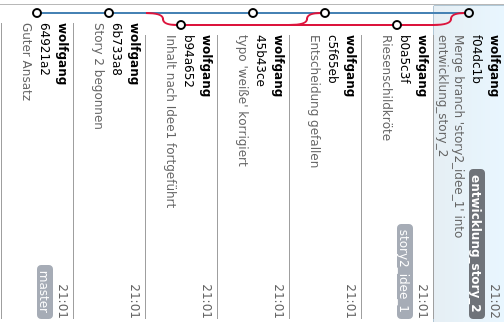
\includegraphics[width=10cm,height=\textheight]{bilder/bash/buch_2.png}

Gut - das war ein langer Weg mit vielen Abzweigungen. Es ist normal,
diesen Abschnitt mehrfach lesen zu müssen!

\subsection{Fazit}\label{fazit}

Branches erlauben gefahrloses Arbeiten an Ideen. Baut man die Szenarien
nicht zu komplex auf, dann gibt auch meist keine Probleme beim Merge.

Immer wenn du Änderungen in einem Zweig vornimmst, die du auch im
anderen Branch menötigst (weiße/weise) kannst du den Merge auch in die
andere Richtung ausführen. Das ist ein übliches Verfahren weil man als
Entwickler immer auf dem aktuellen Stand des Auslieferungszweigs sein
muss, auch wenn er weiter an seinem Experiment arbeitet.

Die Vergleiche mit \emph{diff} sind definitiv gewöhnungsbedürftig.
Machst du häufige Commits auch schon bei kleinen Änderungen, so bekommst
du auch übersichtliche \emph{diffs}.

\begin{Shaded}
\begin{Highlighting}[]
\FunctionTok{git}\NormalTok{ diff }\OperatorTok{\textless{}}\NormalTok{commit}\OperatorTok{\textgreater{}}\NormalTok{..}\OperatorTok{\textless{}}\NormalTok{commit}\OperatorTok{\textgreater{}} \OperatorTok{\textless{}}\NormalTok{datei}\OperatorTok{\textgreater{}}
\end{Highlighting}
\end{Shaded}

Der Nachteil von vielen Commits sind allerdings \ldots{} viele Commits.
Es gibt allerdings Möglichkeiten nachträglich Commits zusammenzufassen
um die Entwicklungsgeschichte zu verschlanken. Diesen Vorgang nennt man
\emph{squashen}.

\bookmarksetup{startatroot}

\chapter{Merge, Rebase, Squash}\label{merge-rebase-squash}

Im letzten Abschnitt hast du einfaches Arbeiten mit Branches gelernt und
wie man sie mit Hilfe eines \emph{Merge} zusammengeführt. Das wollen wir
uns jetzt genauer ansehen. Offen geblieben sind aber folgende Fragen:

\begin{itemize}
\tightlist
\item
  Was passiert mit alten Branches?
\item
  Was mache ich mit zu vielen Commits?
\item
  Wie sieht die Alternative zu \emph{Merge} aus?
\end{itemize}

\section{Verschiedene Merges}\label{verschiedene-merges}

In der Praxis treten\footnote{Bei mir} meist zwei Fälle auf, da ich in
der Regel alleine entwickle:

\begin{itemize}
\tightlist
\item
  Während ich am Entwicklungs-Branch arbeite, passiert auf dem
  Auslieferungsbranch nichts.
\item
  Ich entwickle an einem völlig anderen Feature, das den
  Auslieferungsbranch gar nicht betrifft. Weil das oft aus Zeitgründen
  länger dauert, kann es im Auslieferungsbranch Änderungen geben, die im
  Entwicklungsbranch nicht interessieren.
\end{itemize}

\subsection{Fast-Forward}\label{fast-forward}

Ohne Änderung im Auslieferungsbranch wird der der Entwicklungsbranch
einfach (schnell davor) vor den letzten Commit des Auslieferungsbranchs
gesetzt. In dieser Situation wird im Diagramm der Branch nicht einmal
als visuelle Abzweigung dargestellt:

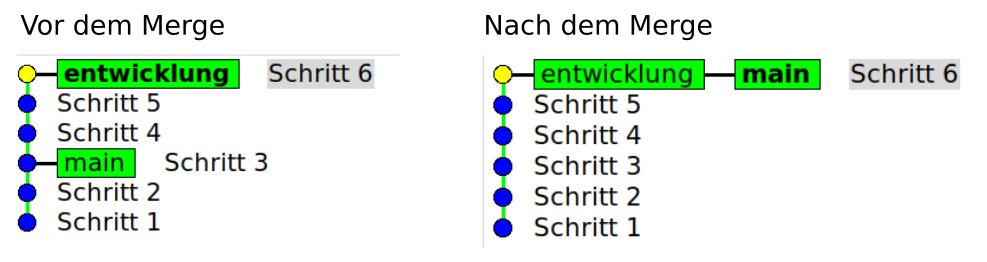
\includegraphics[width=16cm,height=\textheight]{bilder/bash/fast_forward.png}

Erkennbar sind die grünen Rechtecke, die die Enden der Branches
kennzeichnen. Im Bild links sind die Branches getrennt, im Bild rechts
sind beide Branch-Enden nach dem Merge an der gleichen Stelle.\\
Wie du siehst, hat sich beim Merge die Anzahl Commits nicht verändert.

\subsection{Drei-Wege Merge}\label{drei-wege-merge}

Wenn sich der Auslieferungsbranch parallel zum Entwicklungsbranch
weiterentwickelt, sieht die Sitation ganz anders aus!

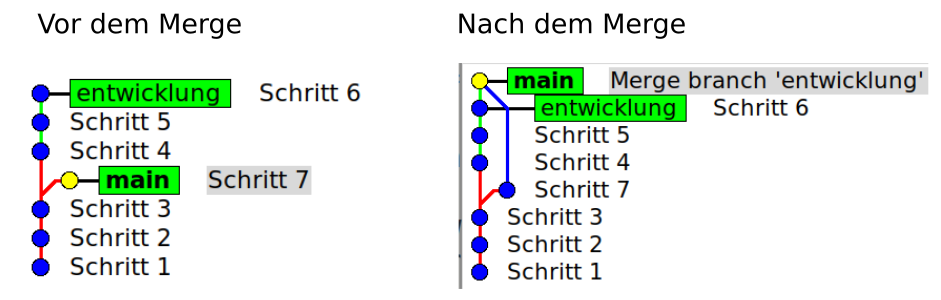
\includegraphics{bilder/bash/drei_wege.png}

Du siehst, dass sich der \emph{main}-Branch zu \emph{Schritt 7}
weiterentwickelt hat. Beim Merge entsteht ein neuer Commit, der die
Spitze beider Branches darstellt. Du erkennst auch, dass im Diagramm die
grünen Spitzen der Branches nicht am gleichen Commit sitzen!

Durch \texttt{git\ log\ -\/-oneline\ -\/-decorate\ -\/-graph} (merken
als „git log dog``) wird diese Sitation auch passend dargestellt:

\begin{Shaded}
\begin{Highlighting}[]
\ExtensionTok{*}\NormalTok{   70c1b21 }\ErrorTok{(}\ExtensionTok{HEAD} \AttributeTok{{-}}\OperatorTok{\textgreater{}}\NormalTok{ main}\KeywordTok{)} \ExtensionTok{Merge}\NormalTok{ branch }\StringTok{\textquotesingle{}entwicklung\textquotesingle{}}\NormalTok{ into main}
\KeywordTok{|}\ExtensionTok{\textbackslash{} } 
\KeywordTok{|} \ExtensionTok{*}\NormalTok{ 4a6e3a5 }\ErrorTok{(}\ExtensionTok{entwicklung}\KeywordTok{)} \ExtensionTok{Schritt}\NormalTok{ 6}
\KeywordTok{|} \ExtensionTok{*}\NormalTok{ edaeaff Schritt 5}
\KeywordTok{|} \ExtensionTok{*}\NormalTok{ 508019b Schritt 4}
\ExtensionTok{*} \KeywordTok{|} \ExtensionTok{2ff4a45}\NormalTok{ Schritt 7}
\KeywordTok{|}\ExtensionTok{/}  
\ExtensionTok{*}\NormalTok{ 29d2bd4 Schritt 3}
\ExtensionTok{*}\NormalTok{ 964ee6f Schritt 2}
\ExtensionTok{*}\NormalTok{ 66dcd4f Schritt 1}
\end{Highlighting}
\end{Shaded}

\section{Alte Branches}\label{alte-branches}

Die Commits eines Branches stellen eine Dokumentation des
Projektverlaufes dar, die für das Verständnis der erfolgten Änderungen
eventuell notwendig sind. Zu viele Branches und Commits erschweren auf
der anderen Seite den Überblick.

Es geht also darum, alte Branches zu löschen, die \emph{wichtigen}
Commits aber zu behalten. Für den schulischen ist das aber weniger
relevant.

Um einen lokalen Branch zu löschen, gibt es folgenden Befehl:

\begin{Shaded}
\begin{Highlighting}[]
\FunctionTok{git}\NormalTok{ branch }\AttributeTok{{-}d} \OperatorTok{\textless{}}\NormalTok{name}\OperatorTok{\textgreater{}}
\end{Highlighting}
\end{Shaded}

Er scheitert aber, wenn \git den Branch noch nicht als abgeschlossen
betrachtet.

Probieren wir das beim letzten Szenario aus. Sieh dir die Abbildung oben
nich einmal an und dann lösche den Branche

\begin{Shaded}
\begin{Highlighting}[]
\FunctionTok{git}\NormalTok{ branch }\AttributeTok{{-}d}\NormalTok{ entwicklung }
\end{Highlighting}
\end{Shaded}

Du siehst eine minimale Änderung

\begin{Shaded}
\begin{Highlighting}[]
\ExtensionTok{*}\NormalTok{   70c1b21 }\ErrorTok{(}\ExtensionTok{HEAD} \AttributeTok{{-}}\OperatorTok{\textgreater{}}\NormalTok{ main}\KeywordTok{)} \ExtensionTok{Merge}\NormalTok{ branch }\StringTok{\textquotesingle{}entwicklung\textquotesingle{}}\NormalTok{ into main}
\KeywordTok{|}\ExtensionTok{\textbackslash{} } 
\KeywordTok{|} \ExtensionTok{*}\NormalTok{ 4a6e3a5 Schritt 6   }\OperatorTok{\textless{}\textless{}\textless{}}\NormalTok{ hier fehlt }\ErrorTok{(}\ExtensionTok{entwicklung}\KeywordTok{)}
\KeywordTok{|} \ExtensionTok{*}\NormalTok{ edaeaff Schritt 5}
\KeywordTok{|} \ExtensionTok{*}\NormalTok{ 508019b Schritt 4}
\ExtensionTok{*} \KeywordTok{|} \ExtensionTok{2ff4a45}\NormalTok{ Schritt 7}
\KeywordTok{|}\ExtensionTok{/}  
\ExtensionTok{*}\NormalTok{ 29d2bd4 Schritt 3}
\ExtensionTok{*}\NormalTok{ 964ee6f Schritt 2}
\ExtensionTok{*}\NormalTok{ 66dcd4f Schritt 1}
\end{Highlighting}
\end{Shaded}

Das \emph{Etikett} vom Entwicklungsbranch wurde gelöscht, die Commits
bleiben aber in exakt der gleichen Anordnung erhalten! Der Branch ist
nicht mehr über seinen Namen zugänglich, die History ist aber weiterhin
vorhanden.

\section{Rebase}\label{rebase}

Neben dem \emph{Merge} trifft man auch oft auf den \emph{Rebase} um
Branches zusammenzuführen. Er funktioniert allerdings deutlich anders
und ist wegen seiner vielfältigen Möglichkeiten (z.B. Reihenfolge der
Commits ändern, \ldots) ein Werkzeug für fortgeschrittene Benutzer. Mit
seiner Hilfe können auch mehrere Commits zusammengefasst werden, um die
Branches zu verkürzen. Gerade bei der Zusammenarbeit im Team kann das
aber sehr problematisch werden, wenn man nicht genau weiß, was man
macht. Das liegt daran, dass sich die Hashwerte von Commits ändern
können und wenn sich ein anderer Mitarbeiter den früheren Stand kopiert
hat, dann kann das zu großem Chaos führen.

https://www.youtube.com/watch?v=CtyLg10aHN0
https://www.youtube.com/watch?v=1TNK-OkaelI

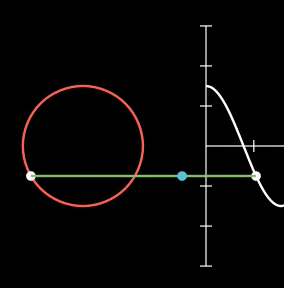
\includegraphics{bilder/bash/rebase_nach_branch_delete.png}

Bei einem Rebase wird der entsprechende Branch \emph{verpflanzt} -- d.h.
gewissermaßen \emph{ausgerupft} und an anderer Stelle wieder
\emph{angedockt}.\\
Bei diesem Vorgang werden die Hashwerte aller Commits im Branch
geändert.

\begin{Shaded}
\begin{Highlighting}[]
\ExtensionTok{*}\NormalTok{ 10f8d8d }\ErrorTok{(}\ExtensionTok{HEAD} \AttributeTok{{-}}\OperatorTok{\textgreater{}}\NormalTok{ arbeit}\KeywordTok{)} \ExtensionTok{Neuer}\NormalTok{ Inhalt 10}
\ExtensionTok{*}\NormalTok{ e0ae3ce Neuer Inhalt 9}
\ExtensionTok{*}\NormalTok{ 1eac6f3 Neuer Inhalt 8}
\ExtensionTok{*}\NormalTok{ fa76537 Neuer Inhalt 7}
\ExtensionTok{*}\NormalTok{ da22859 Neuer Inhalt 6}
\ExtensionTok{*}\NormalTok{ 7903aaf Neuer Inhalt 5}
\ExtensionTok{*}\NormalTok{ 33428f1 Neuer Inhalt 4}
\ExtensionTok{*}\NormalTok{ 80db22a Neuer Inhalt 3}
\ExtensionTok{*}\NormalTok{ 4a642a8 Neuer Inhalt 2}
\ExtensionTok{*}\NormalTok{ a3645f3 Neuer Inhalt 1}
\KeywordTok{|} \ExtensionTok{*}\NormalTok{ 2c58be7 }\ErrorTok{(}\ExtensionTok{main}\KeywordTok{)} \ExtensionTok{Zwischenstopp}
\KeywordTok{|}\ExtensionTok{/}  
\ExtensionTok{*}\NormalTok{ 7fea00c Start}
\end{Highlighting}
\end{Shaded}

Du siehst einen Branch \branch{arbeit} mit mehreren Commits und einen
neuen Commit im \branch{main}-Branch.

Wenn du nun vom Branch \branch{arbeit} einen Rebase auf den Branch
\branch{main} ausführst:

\begin{Shaded}
\begin{Highlighting}[]
\FunctionTok{git}\NormalTok{ switch arbeit }
\FunctionTok{git}\NormalTok{ rebase main }
\end{Highlighting}
\end{Shaded}

dann sieht das Ergebnis so aus:

\begin{Shaded}
\begin{Highlighting}[]
\ExtensionTok{*}\NormalTok{ 1cad272 }\ErrorTok{(}\ExtensionTok{HEAD} \AttributeTok{{-}}\OperatorTok{\textgreater{}}\NormalTok{ arbeit}\KeywordTok{)} \ExtensionTok{Neuer}\NormalTok{ Inhalt 10}
\ExtensionTok{*}\NormalTok{ 130c5b0 Neuer Inhalt 9}
\ExtensionTok{*}\NormalTok{ 5b84ab1 Neuer Inhalt 8}
\ExtensionTok{*}\NormalTok{ 56d74ea Neuer Inhalt 7}
\ExtensionTok{*}\NormalTok{ 9255c1d Neuer Inhalt 6}
\ExtensionTok{*}\NormalTok{ 412fa37 Neuer Inhalt 5}
\ExtensionTok{*}\NormalTok{ cb91e55 Neuer Inhalt 4}
\ExtensionTok{*}\NormalTok{ 3ab37b7 Neuer Inhalt 3}
\ExtensionTok{*}\NormalTok{ dc4b1b0 Neuer Inhalt 2}
\ExtensionTok{*}\NormalTok{ 9591035 Neuer Inhalt 1}
\ExtensionTok{*}\NormalTok{ 2c58be7 }\ErrorTok{(}\ExtensionTok{main}\KeywordTok{)} \ExtensionTok{Zwischenstopp}
\ExtensionTok{*}\NormalTok{ 7fea00c Start}
\end{Highlighting}
\end{Shaded}

Die Verzeigung ist verschwunden und der Branch \branch{arbeit} hängt mit
seinen Commits und neuen Hashwerten\\
am Commit mit dem Hash 2c58be7 aus dem Branch \branch{main}.

Auch wenn es nicht so wirkt: Der Branch \branch{arbeit} ist immer noch
vorhanden! Das kannst du auch einfach testen, indem du auf den
\branch{main}-Branch wechselst und dort einen neuen Commit erstellst:

\begin{Shaded}
\begin{Highlighting}[]
\FunctionTok{git}\NormalTok{ switch main }
\BuiltInTok{echo} \StringTok{"kontrolle"} \OperatorTok{\textgreater{}}\NormalTok{ kontrolle.txt }
\FunctionTok{git}\NormalTok{ add kontrolle.txt }
\FunctionTok{git}\NormalTok{ commit }\AttributeTok{{-}m} \StringTok{"Kontrolle"}
\end{Highlighting}
\end{Shaded}

Das Log zeigt dann

\begin{Shaded}
\begin{Highlighting}[]
\ExtensionTok{*}\NormalTok{ 3508cce }\ErrorTok{(}\ExtensionTok{HEAD} \AttributeTok{{-}}\OperatorTok{\textgreater{}}\NormalTok{ main}\KeywordTok{)} \ExtensionTok{kkkddd}
\KeywordTok{|} \ExtensionTok{*}\NormalTok{ f4ba9f7 }\ErrorTok{(}\ExtensionTok{arbeit}\KeywordTok{)} \ExtensionTok{kkk}
\KeywordTok{|} \ExtensionTok{*}\NormalTok{ 1cad272 Neuer Inhalt 10}
\ExtensionTok{....}
\KeywordTok{|} \ExtensionTok{*}\NormalTok{ dc4b1b0 Neuer Inhalt 2}
\KeywordTok{|} \ExtensionTok{*}\NormalTok{ 9591035 Neuer Inhalt 1}
\KeywordTok{|}\ExtensionTok{/}  
\ExtensionTok{*}\NormalTok{ 2c58be7 Zwischenstopp}
\ExtensionTok{*}\NormalTok{ 7fea00c Start}
\end{Highlighting}
\end{Shaded}

Die Branches laufen also wieder auseinander. Möchte man den Branch
\branch{arbeit} loswerden, dann würdest du hier eher den Rebase von
\branch{main} auf \branch{arbeit} ausführen. \git versucht dann, den
\branch{main}-Branch hinter den Branch \branch{arbeit} zu hängen. Aus
dieser Situation heraus kannst du dann auch den Branch \branch{arbeit}
löschen:

\begin{Shaded}
\begin{Highlighting}[]
\FunctionTok{git}\NormalTok{ branch }\AttributeTok{{-}d}\NormalTok{ arbeit }
\end{Highlighting}
\end{Shaded}

\bookmarksetup{startatroot}

\chapter{Arbeiten im Team}\label{arbeiten-im-team}

\section{Herausforderungen}\label{herausforderungen}

Das Arbeiten im Team stellt dich vor zwei Probleme

\begin{itemize}
\tightlist
\item
  Welche Server-Infrastruktur sollst du verwenden?
\item
  Was ändert sich am Workflow in \git 
\end{itemize}

Beide Punkte sollen nachfolgend besprochen werden, wobei es zwangsläufig
Überschneidungen geben wird.

\subsection{Infrastruktur}\label{infrastruktur}

Im Kern ist es egal ob wir vom Setup im Klassenzimmer oder im Internet
sprechen -- sobald ein Netzwerk beteiligt ist, sind höchstens
Sicherheitsaspekte ein Thema, die Basistechnik bleibt gleich.

Für eine servbasierende Teamarbeit gibt es folgende Varianten

\begin{itemize}
\item
  einfacher \git-Server\\
  Die Installation ist einfach, die Grundkonfiguration auch. Der Zugriff
  erfolgt über ssh. Soll das ohne Kennwort funktionieren, so müssen
  Schlüssel erzeugt und auf den Server eingepflegt werden. Sspäter führt
  um die Schlüssel aber kein Weg herum.
\item
  \git-Server mit kennwortlosem Zgriff über http.\\
  Funktioniert, ist aber keinesfalls für den Live-Einsatz über einen
  längeren Zeitraum im Internet zu empfehlen. Die entsprechenden
  Docker-Files befinden sich in den Materialien. (Basis:
  \href{https://github.com/ynohat/git-http-backend}{ynohat} )
\item
  Ein \git-Server mit \emph{Gitea}\\
  Gui-basiertes System mit vielen Optionen und weniger komplex als
  \emph{GitLab}
\item
  Ein \git-Server mit \emph{GitLab}
\end{itemize}

Bei allen Varianten ist im Prinzip eine direkte Installation auf den
Server (nicht empfohlen) oder der Einsatz von Docker (sinnvoll) möglich.
Die Anleitungen für die einzelnen Varianten befinden sich weiter hinten
im Script.

\subsection{Überblick}\label{uxfcberblick}

Bei der Arbeit im Team ändert sich beim lokalen Arbeiten zunächst wenig.
Die Schritte \emph{branch, add, commit, \ldots{}} funktionieren wie auch
bisher. Neu sind allerdings die Schritte

\begin{itemize}
\tightlist
\item
  Initiales Holen des Repos auf den eigenen Rechner (=clone)
\item
  Regelmäßiges Abrufen des aktuellen Standes (=pull)
\item
  Veröffentlichen des eigenen Standes (push)
\end{itemize}

Hierbei sind einige Spielregeln zu beachten, damit es nicht zu Problemen
kommt. Diese Regeln werden meist als Workflow oder im Speziellen auch
als GitFlow bezeichnet. Es gibt hier zwar gewisse -- aber keinesfalls
verbindliche -- Standards. Jede Firma stellt hier ihre eigenen, fest
vorgeschriebenenen Abläufe auf, an die sie die Mitarbeiter zu halten
haben.

\subsubsection{Gemeinsamkeiten}\label{gemeinsamkeiten}

Auch diese Gemeinsamkeiten müssen nicht in jeder Firma oder jedem
Projekt umgesetzt werden!

\textbf{Verantwortung}\\
Im Projekt gibt es einen \branch{main}, der aber durch entsprechende
Maßnahmen für \emph{einfache} Mitarbeiter schreibgeschützt ist.
Änderungen dürfen nur nach gründlichen Tests und Code-Reviews in diesen
Zweig aufgenommen werden. In der Regel gilt hier auch ein
\emph{Mehr-Augen-Prinzip} oder noch weiter gestaffelte
Zuständigkeitshierarchien.

\textbf{Arbeitsbranch}\\
Je nach Größe des Projekt-Teams gibt es einen oder mehrere
\branch{development}-Branches. Die Mitarbeiter holen sich diesen Zweig
und lassen von ihm ihre eigenen Arbeitszweige (Feature-Branches,
Bugfix-Branches) ausgehen. Ist ihre Arbeit dort beendet, muss der Code
getestet werden und dann erst erfolgt der Merge in den
\branch{development}-Branch.

\subsubsection{Details}\label{details}

Da jetzt mehr Personen Änderungen zu unvorhersehbaren Zeitpunkten
Änderungen am Code vornehmen, muss jeder Mitarbeiter dafür sorgen, immer
die aktuellste Version vorliegen zu haben. Da er seine Entwicklung aber
in seinem eigenen \branch{Feature}-Branch vorantreibt, müssen diese
Änderungen dort aber erst ankommen -- dies geschieht durch Merges in die
andere Richtung!

\textbf{Beispiel}

Aus Platzgründen zeichne ich das Branch-Diagramm hier waagrecht. Der
\branch{feature}-Branch ist auch noch nicht so weit fortgeschritten, als
dass ein Merge auf den \branch{development}-Branch erfolgt wäre.



\begin{tikzpicture}[scale=0.8]

\draw(0,0) rectangle ++(16,6);

\begin{scope}[]
\draw(1,1) -- (13,1);
\draw[fill=red!20]
(1,1) circle (0.5) node [  ]   { m1  }   ++ 
(2,0) circle (0.5) node [  ]   { m2  }   ++
(2,0) circle (0.5) node [  ]   { m3  }   ++ 
(2,0) circle (0.5) node [  ]   { m4  }   ++ 
(2,0) circle (0.5) node [  ]   { m5  }   ++ 
(2,0) circle (0.5) node [  ]   { m6  } ; 
\draw(14,1) node[scale=1.2]{main};
\end{scope}


\begin{scope}[yshift=2cm, xshift=3cm]
\draw(1,1) -- (9,1);
\draw[fill=red!20]
(1,1) circle (0.5) node [  ]   { d1  }   ++ 
(2,0) circle (0.5) node [  ]   { d2  }   ++
(2,0) circle (0.5) node [  ]   { d3  }   ++ 
(2,0) circle (0.5) node [  ]   { d4  }  ;
\draw(11,1) node[scale=1.2]{development};
\end{scope}


\draw(3.2,1.45) -- ++ (60:1.25);
\draw(5.2,1.45) -- ++ (60:1.25);
\draw(7.2,1.45) -- ++ (60:1.25);



\begin{scope}[yshift=4cm, xshift=5cm]
\draw(1,1) -- (9,1);
\draw[fill=red!20]
(1,1) circle (0.5) node [  ]   { f1  }   ++ 
(2,0) circle (0.5) node [  ]   { f2  }   ++
(2,0) circle (0.5) node [  ]   { f3  }   ++ 
(2,0) circle (0.5) node [  ]   { f4  }  ;
\draw(10,1) node[scale=1.2]{feature};
\end{scope}

\draw(4.4,3.28) -- ++ (48:1.85);
\draw(6.4,3.28) -- ++ (48:1.85);
\draw(8.4,3.28) -- ++ (48:1.85);


\end{tikzpicture}

Da noch keine wirklichen Fortschritte erzielt worden sind, dürfte der
\branch{development}-Branch auch noch nicht wieder auf den Server
veröffentlicht worden sein (=push).

\subsubsection{Pull und fetch}\label{pull-und-fetch}

Die Grundidee von \emph{holen} und \emph{veröffentlichen} ist relativ
einfach und eventuell muss man den Schülern auch nicht mehr erzählen. Da
aber Code von anderen Entwicklern auf deinen Rechner kommt, solltest du
diesen eventuell nicht ungesehen in deine Entwicklung aufnehmen.
\cmd{git pull} macht aber genau das.\\
Willst du an dieser Stelle sicher gehen, so machst du zuerst
\cmd{git fetch} und siehst dir die Änderungen zuerst an -- siehe weiter
unten. Im Anschluss kannst du sie dann mit \cmd{git merge} übernehmen.

\section{Hands on}\label{hands-on-1}

In den nachfolgenden Abschnitten wird oft das Wort \emph{origin}
auftreten. Wir sehen uns lieber gleich an, was es damit auf sich hat.
Für die einzelnen Schritte gibt es Scripts in den Kursmaterialien!

\subsection{origin}\label{origin}

\textbf{Origin.sh}

\begin{Shaded}
\begin{Highlighting}[]
\CommentTok{\#!/bin/bash}

\CommentTok{\# Putzen}
\ControlFlowTok{if} \BuiltInTok{[} \OtherTok{{-}d}\NormalTok{ labor1 }\BuiltInTok{]}
\ControlFlowTok{then} 
  \FunctionTok{rm} \AttributeTok{{-}rf}\NormalTok{ labor1}
\ControlFlowTok{fi} 

\CommentTok{\# Anlegen}
\FunctionTok{mkdir}\NormalTok{ labor1}
\BuiltInTok{cd}\NormalTok{ labor1}

\VariableTok{AKTUELL}\OperatorTok{=}\VariableTok{$PWD}  \CommentTok{\# Pfad merken}

\CommentTok{\# Repo "entfernt.git" anlegen}
\FunctionTok{git}\NormalTok{ init }\AttributeTok{{-}{-}bare}\NormalTok{ entfernt.git}
\CommentTok{\# branch auf main umbenennen}
\BuiltInTok{cd}\NormalTok{ entfernt.git}
\FunctionTok{git}\NormalTok{ branch }\AttributeTok{{-}m}\NormalTok{ main}
\BuiltInTok{cd}\NormalTok{ ..}

\CommentTok{\# Repo in Ordner "lokal" clonen}
\FunctionTok{git}\NormalTok{ clone }\VariableTok{$AKTUELL}\NormalTok{/entfernt.git lokal}

\CommentTok{\# Überblick}
\BuiltInTok{cd}\NormalTok{ lokal}
\FunctionTok{git}\NormalTok{ status}
\end{Highlighting}
\end{Shaded}

Das Script \script{origin.sh} erstellt dir

\begin{itemize}
\tightlist
\item
  Ein Repository \emph{entfernt}, das einen Server darstellt
\item
  Ein Repository \emph{lokal}, das deinen Rechner darstellt, indem es
  eine Kopie von \emph{entfernt} erstellt (=clone).
\end{itemize}

Öffne eine \git-Bash in einem Spielordner und führe das Script
\script{origin.sh} aus. Die Ausgabe wird bei dir minimal abweichen.

\begin{Shaded}
\begin{Highlighting}[]
\ExtensionTok{Leeres}\NormalTok{ Git{-}Repository in /tmp/labor1/entfernt.git/ initialisiert}
\ExtensionTok{Klone}\NormalTok{ nach }\StringTok{\textquotesingle{}lokal\textquotesingle{}}\NormalTok{ …}
\ExtensionTok{warning:}\NormalTok{ Sie scheinen ein leeres Repository geklont zu haben.}
\ExtensionTok{Fertig.}
\ExtensionTok{Auf}\NormalTok{ Branch main}

\ExtensionTok{Noch}\NormalTok{ keine Commits}

\ExtensionTok{nichts}\NormalTok{ zu committen }\ErrorTok{(}\ExtensionTok{erstellen/kopieren}\NormalTok{ Sie Dateien und benutzen}
\ExtensionTok{Sie} \StringTok{"git add"}\NormalTok{ zum Versionieren}\KeywordTok{)}
\end{Highlighting}
\end{Shaded}

Durch

\begin{Shaded}
\begin{Highlighting}[]
\FunctionTok{git}\NormalTok{ remote }\AttributeTok{{-}v} 
\end{Highlighting}
\end{Shaded}

siehst du, woher das Repository stammt. Bei dir ist natürlich ein
anderer Pfad zu sehen!

\begin{Shaded}
\begin{Highlighting}[]
\ExtensionTok{origin}\NormalTok{  /tmp/labor1/entfernt.git }\ErrorTok{(}\ExtensionTok{fetch}\KeywordTok{)}
\ExtensionTok{origin}\NormalTok{  /tmp/labor1/entfernt.git }\ErrorTok{(}\ExtensionTok{push}\KeywordTok{)}
\end{Highlighting}
\end{Shaded}

Wenn also in den folgenden Ausgaben und Befehlen \emph{origin}
erscheint, dann ist dieser Pfad gemeint. \emph{Pfad} kann allerdings
auch eine Netzwerkverbindung zu einem Server sein -- das ist sogar der
Normalfall.

Mit \branch{origin/main} ist immer der Branch im entfernten Repository
gemeint, \branch{main} alleine bezieht sich auf den Branch in deiner
lokalen Kopie.

\subsection{Zeiger}\label{zeiger}

Der nachfolgende Setup erstellt

\begin{itemize}
\tightlist
\item
  einen Ordner
\item
  im Ordner ein vollwertiges Repository (--bare)
\item
  eine lokale Kopie des Repositories mit dem Namen \emph{susi}
\item
  eine lokale Kopie des Repositories mit dem Namen \emph{max}
\end{itemize}

Öffen in einem geeigneten Ordner ein \git-Bash und führe das Script
\script{susi\_und\_max.sh} aus (\script{}./susi\_und\_max.sh\}).

Beachte, dass aus in dem Script im oberen Teil etwas Overhead nötig ist,
damit die Benutzer nicht mit einem leeren Repository konfrontiert werden
-- dort fehlt dann nämlich ein Branch!

\begin{Shaded}
\begin{Highlighting}[]
\CommentTok{\#!/bin/bash}

\CommentTok{\# Putzen}
\ControlFlowTok{if} \BuiltInTok{[} \OtherTok{{-}d}\NormalTok{ labor2 }\BuiltInTok{]}
\ControlFlowTok{then} 
  \FunctionTok{rm} \AttributeTok{{-}rf}\NormalTok{ labor2}
\ControlFlowTok{fi} 

\CommentTok{\# Anlegen}
\FunctionTok{mkdir}\NormalTok{ labor2}
\BuiltInTok{cd}\NormalTok{ labor2}

\FunctionTok{git}\NormalTok{ init }\AttributeTok{{-}{-}bare}\NormalTok{ entfernt.git}
\BuiltInTok{cd}\NormalTok{ entfernt.git}
\FunctionTok{git}\NormalTok{ branch }\AttributeTok{{-}m}\NormalTok{ main}
\BuiltInTok{cd}\NormalTok{ ..}

\VariableTok{ARBEIT}\OperatorTok{=}\VariableTok{$PWD}  \CommentTok{\# aktuellen Pfad merken }
\VariableTok{SUSI}\OperatorTok{=}\VariableTok{$ARBEIT}\NormalTok{/susi  }\CommentTok{\# Abkürzungen für den Überblick  }
\VariableTok{MAX}\OperatorTok{=}\VariableTok{$ARBEIT}\NormalTok{/max}

\CommentTok{\# Overhead}
\FunctionTok{git}\NormalTok{ clone }\VariableTok{$ARBEIT}\NormalTok{/entfernt vorbereitung}
\BuiltInTok{cd}\NormalTok{ vorbereitung}
\BuiltInTok{echo} \StringTok{"Hi"} \OperatorTok{\textgreater{}}\NormalTok{ README.md}
\FunctionTok{git}\NormalTok{ add README.md}
\FunctionTok{git}\NormalTok{ commit }\AttributeTok{{-}m} \StringTok{"Init"}
\FunctionTok{git}\NormalTok{ push }\AttributeTok{{-}u}\NormalTok{ origin main}
\BuiltInTok{cd}\NormalTok{ ..}
\FunctionTok{rm} \AttributeTok{{-}rf}\NormalTok{ vorbereitung}

\FunctionTok{git}\NormalTok{ clone }\VariableTok{$ARBEIT}\NormalTok{/entfernt susi }
\FunctionTok{git}\NormalTok{ clone }\VariableTok{$ARBEIT}\NormalTok{/entfernt max   }

\CommentTok{\#}
\CommentTok{\#cd $SUSI }
\CommentTok{\#echo "Hallo" \textgreater{} datei.txt }
\CommentTok{\#git add datei.txt }
\CommentTok{\#git commit {-}m "Hallo geschrieben"}

\CommentTok{\#git branch {-}m main }
\end{Highlighting}
\end{Shaded}

Öffne ein zweites Fenster im gleichen Ordner und entscheide dich,
welches für \emph{Susi} und welches für \emph{Max} stehen soll. Wechsle
jeweils in das Repository (\cmd{cd susi} und \cmd{cd max}).

Lasse dir in beiden Repositories den Status ausgeben

\begin{Shaded}
\begin{Highlighting}[]
\FunctionTok{git}\NormalTok{ status}
\end{Highlighting}
\end{Shaded}

Es sollte jeweils erscheinen

\begin{Shaded}
\begin{Highlighting}[]
\ExtensionTok{Auf}\NormalTok{ Branch main}
\ExtensionTok{Ihr}\NormalTok{ Branch ist auf demselben Stand wie }\StringTok{\textquotesingle{}origin/main\textquotesingle{}}\NormalTok{.}

\ExtensionTok{nichts}\NormalTok{ zu committen, Arbeitsverzeichnis unverändert}
\end{Highlighting}
\end{Shaded}

Im Prinzip hat Susi jetzt eine identische Kopie des Repositories
erstellt. Allerdings ist der \branch{main}-Branch jetzt \emph{Susis}
\branch{main}-Branch in \emph{diesem} Repository. Die Statusmeldung sagt
dir, beide Branches \emph{main} (Susis) und \emph{origin/main} (der im
Original Repo) sind gleich.

Nachfolgend stehen die Bezeichnungen \emph{Original} und \emph{SUSI}
bzw. \emph{MAX} für die entsprechenden Repositories.

Susi erstellt in \emph{SUSI} eine Datei und einen Commit:

\begin{Shaded}
\begin{Highlighting}[]
\BuiltInTok{echo} \StringTok{"Hallo Welt"} \OperatorTok{\textgreater{}\textgreater{}}\NormalTok{ datei.txt }
\FunctionTok{git}\NormalTok{ add datei.txt }
\FunctionTok{git}\NormalTok{ commit }\AttributeTok{{-}m} \StringTok{"Begrüßung"}
\end{Highlighting}
\end{Shaded}

und betrachtet den Status erneut:

\begin{Shaded}
\begin{Highlighting}[]
\ExtensionTok{Auf}\NormalTok{ Branch main}
\ExtensionTok{Ihr}\NormalTok{ Branch ist 1 Commit vor }\StringTok{\textquotesingle{}origin/main\textquotesingle{}}\NormalTok{.}
  \KeywordTok{(}\ExtensionTok{benutzen}\NormalTok{ Sie }\StringTok{"git push"}\NormalTok{, um lokale Commits zu publizieren}\KeywordTok{)}

\ExtensionTok{nichts}\NormalTok{ zu committen, Arbeitsverzeichnis unverändert}
\end{Highlighting}
\end{Shaded}

Der \git-Ordner führt also Buch über die Beziehung zwischen den
Repositories und sagt ihr, dass \emph{SUSI} einen Commit weiter vorne
ist, als das \emph{Original}.\\
Das macht \git, indem es \emph{Pointer} auf Commits setzt (also quasi
eine Datei im \ordner{.git}-Ordner führt, wo der aktuelle Hash enthalten
ist.)

\phantomsection\label{annotated-cell-82}%
\begin{Shaded}
\begin{Highlighting}[]
\ExtensionTok{...}
\ExtensionTok{├──}\NormalTok{ config}
\ExtensionTok{├──}\NormalTok{ description}
\ExtensionTok{├──}\NormalTok{ HEAD }\hspace*{\fill}\NormalTok{\circled{1}}
\ExtensionTok{├──}\NormalTok{ hooks}
\ExtensionTok{│  }\NormalTok{ ├── applypatch{-}msg.sample}
\ExtensionTok{...}
\ExtensionTok{├──}\NormalTok{ packed{-}refs }\hspace*{\fill}\NormalTok{\circled{3}}
\ExtensionTok{└──}\NormalTok{ refs}
    \ExtensionTok{├──}\NormalTok{ heads}
    \ExtensionTok{│  }\NormalTok{ └── main}
    \ExtensionTok{├──}\NormalTok{ remotes}
    \ExtensionTok{│  }\NormalTok{ └── origin}
    \ExtensionTok{│  }\NormalTok{     └── HEAD }\hspace*{\fill}\NormalTok{\circled{2}}
    \ExtensionTok{└──}\NormalTok{ tags}
\end{Highlighting}
\end{Shaded}

\begin{description}
\tightlist
\item[\circled{1}]
Enthält den Hash vom letzten Commit in der lokalen Kopie
\item[\circled{2}]
Enthält den Hash vom letzten Commit im Original
\item[\circled{3}]
Siehe nachfolgender Text
\end{description}

Ein \cmd{git log --oneline} zeigt dir:

\begin{Shaded}
\begin{Highlighting}[]
\ExtensionTok{78db34e} \ErrorTok{(}\ExtensionTok{HEAD} \AttributeTok{{-}}\OperatorTok{\textgreater{}}\NormalTok{ main}\KeywordTok{)} \ExtensionTok{Begrüßung}
\ExtensionTok{d46681d} \ErrorTok{(}\ExtensionTok{origin/main,}\NormalTok{ origin/HEAD}\KeywordTok{)} \ExtensionTok{Init}
\end{Highlighting}
\end{Shaded}

Und ein Blick in die beiden Dateien liefert die Hashes -- zumindest
fast, denn \git hat hier schon wieder optimiert und den Hash vom
\emph{origin/master} in die Datei \emph{packed-refs} umgelagert.

Das \emph{Original} weiß von diesem Commit noch nichts -- die
Repositories haben ja auch noch nicht miteinander kommuniziert! Wenn Max
in seinem Repository \emph{MAX} nachsieht kann er Susis Datei nicht
sehen und daran würde auch ein \cmd{git pull} nichts ändern.

Susi führt nun einen Push aus:

\begin{Shaded}
\begin{Highlighting}[]
\FunctionTok{git}\NormalTok{ push origin main }
\end{Highlighting}
\end{Shaded}

\emph{Git} kommentiert das:

\begin{Shaded}
\begin{Highlighting}[]
\ExtensionTok{Objekte}\NormalTok{ aufzählen: 4, fertig.}
\ExtensionTok{Zähle}\NormalTok{ Objekte: 100\% }\ErrorTok{(}\ExtensionTok{4/4}\KeywordTok{)}\ExtensionTok{,}\NormalTok{ fertig.}
\ExtensionTok{Delta{-}Kompression}\NormalTok{ verwendet bis zu 6 Threads.}
\ExtensionTok{Komprimiere}\NormalTok{ Objekte: 100\% }\ErrorTok{(}\ExtensionTok{2/2}\KeywordTok{)}\ExtensionTok{,}\NormalTok{ fertig.}
\ExtensionTok{Schreibe}\NormalTok{ Objekte: 100\% }\ErrorTok{(}\ExtensionTok{3/3}\KeywordTok{)}\ExtensionTok{,}\NormalTok{ 292 Bytes }\KeywordTok{|} \ExtensionTok{292.00}\NormalTok{ KiB/s, fertig.}
\ExtensionTok{Gesamt}\NormalTok{ 3 }\ErrorTok{(}\ExtensionTok{Delta}\NormalTok{ 0}\KeywordTok{)}\ExtensionTok{,}\NormalTok{ Wiederverwendet 0 }\ErrorTok{(}\ExtensionTok{Delta}\NormalTok{ 0}\KeywordTok{)}\ExtensionTok{,}\NormalTok{ Pack wiederverwendet 0}
\ExtensionTok{To}\NormalTok{ /tmp/labor2/entfernt}
   \ExtensionTok{d46681d..78db34e}\NormalTok{  main }\AttributeTok{{-}}\OperatorTok{\textgreater{}}\NormalTok{ main}
\end{Highlighting}
\end{Shaded}

und jetzt liefert der Status:

\begin{Shaded}
\begin{Highlighting}[]
\ExtensionTok{Auf}\NormalTok{ Branch main}
\ExtensionTok{Ihr}\NormalTok{ Branch ist auf demselben Stand wie }\StringTok{\textquotesingle{}origin/main\textquotesingle{}}\NormalTok{.}

\ExtensionTok{nichts}\NormalTok{ zu committen, Arbeitsverzeichnis unverändert}
\end{Highlighting}
\end{Shaded}

Die Zeiger in \ordner{.git} wurden also auf den gleichen Hash gesetzt.

\textbf{Wechseln wir zu Max}

Max hat noch sein ursprüngliches Repository und möchte auf Änderungen am
Server prüfen.

\begin{Shaded}
\begin{Highlighting}[]
\FunctionTok{git}\NormalTok{ fetch }
\end{Highlighting}
\end{Shaded}

Als Ausgabe bekommt er

\begin{Shaded}
\begin{Highlighting}[]
\ExtensionTok{remote:}\NormalTok{ Objekte aufzählen: 4, fertig.}
\ExtensionTok{remote:}\NormalTok{ Zähle Objekte: 100\% }\ErrorTok{(}\ExtensionTok{4/4}\KeywordTok{)}\ExtensionTok{,}\NormalTok{ fertig.}
\ExtensionTok{remote:}\NormalTok{ Komprimiere Objekte: 100\% }\ErrorTok{(}\ExtensionTok{2/2}\KeywordTok{)}\ExtensionTok{,}\NormalTok{ fertig.}
\ExtensionTok{remote:}\NormalTok{ Gesamt 3 }\ErrorTok{(}\ExtensionTok{Delta}\NormalTok{ 0}\KeywordTok{)}\ExtensionTok{,}\NormalTok{ Wiederverwendet 0 }\ErrorTok{(}\ExtensionTok{Delta}\NormalTok{ 0}\KeywordTok{)}\ExtensionTok{,}\NormalTok{ Pack wiederverwendet 0}
\ExtensionTok{Entpacke}\NormalTok{ Objekte: 100\% }\ErrorTok{(}\ExtensionTok{3/3}\KeywordTok{)}\ExtensionTok{,}\NormalTok{ 272 Bytes }\KeywordTok{|} \ExtensionTok{272.00}\NormalTok{ KiB/s, fertig.}
\ExtensionTok{Von}\NormalTok{ /tmp/labor2/entfernt}
   \ExtensionTok{d46681d..78db34e}\NormalTok{  main       }\AttributeTok{{-}}\OperatorTok{\textgreater{}}\NormalTok{ origin/main}
\end{Highlighting}
\end{Shaded}

Sein Status sagt ihm

\begin{Shaded}
\begin{Highlighting}[]
\ExtensionTok{Auf}\NormalTok{ Branch main}
\ExtensionTok{Ihr}\NormalTok{ Branch ist 1 Commit hinter }\StringTok{\textquotesingle{}origin/main\textquotesingle{}}\NormalTok{, und kann vorgespult werden.}
  \KeywordTok{(}\ExtensionTok{benutzen}\NormalTok{ Sie }\StringTok{"git pull"}\NormalTok{, um Ihren lokalen Branch zu aktualisieren}\KeywordTok{)}

\ExtensionTok{nichts}\NormalTok{ zu committen, Arbeitsverzeichnis unverändert}
\end{Highlighting}
\end{Shaded}

Mit \emph{vorspulen} ist ein Merge gemeint. Max will aber wissen
\emph{was} sich geändert hat.

\begin{Shaded}
\begin{Highlighting}[]
\FunctionTok{git}\NormalTok{ log origin main}
\end{Highlighting}
\end{Shaded}

Max sieht den Commit, der noch nicht in seinen Branch integriert ist.

\begin{Shaded}
\begin{Highlighting}[]
\ExtensionTok{commit}\NormalTok{ 78db34e3176c4b78d4b027eac06aa4dda5c50cdb }\ErrorTok{(}\ExtensionTok{origin/main,}\NormalTok{ origin/HEAD}\KeywordTok{)}
\ExtensionTok{Author:}\NormalTok{ wolfgang }\OperatorTok{\textless{}}\NormalTok{susi@t{-}online.de}\OperatorTok{\textgreater{}}
\ExtensionTok{Date:}\NormalTok{   Wed Jan 29 12:39:38 2025 +0100}

    \ExtensionTok{Begrüßung}

\ExtensionTok{commit}\NormalTok{ d46681db23c9e2b3f5379a951c026e3d673fe3e0 }\ErrorTok{(}\ExtensionTok{HEAD} \AttributeTok{{-}}\OperatorTok{\textgreater{}}\NormalTok{ main}\KeywordTok{)}
\ExtensionTok{Author:}\NormalTok{ wolfgang }\OperatorTok{\textless{}}\NormalTok{lehrer@t{-}online.de}\OperatorTok{\textgreater{}}
\ExtensionTok{Date:}\NormalTok{   Wed Jan 29 12:34:48 2025 +0100}

    \ExtensionTok{Init}
\end{Highlighting}
\end{Shaded}

Schön sieht man das auch mit

\begin{Shaded}
\begin{Highlighting}[]
\FunctionTok{git}\NormalTok{ show{-}ref}
\end{Highlighting}
\end{Shaded}

Der lokale \branch{main} befindet sich noch bei d46681, der entfernte
\branch{origin main} hingegen bei 78db34.\\
Durch folgenden Befehl sieht Max die Differenz der Versionen:

\begin{Shaded}
\begin{Highlighting}[]
\FunctionTok{git}\NormalTok{ show 78db34}
\end{Highlighting}
\end{Shaded}

Geht es einfach nur um den gesamten Inhalt:

\begin{Shaded}
\begin{Highlighting}[]
\FunctionTok{git}\NormalTok{ show 78db34e3:datei.txt}
\end{Highlighting}
\end{Shaded}

Max erkennt, dass es problemlose Änderungen sind und übernimmt sie in
seinen Branch:

\begin{Shaded}
\begin{Highlighting}[]
\FunctionTok{git}\NormalTok{ merge}
\end{Highlighting}
\end{Shaded}

Die Hashes ziegen, was passiert:

\begin{Shaded}
\begin{Highlighting}[]
\ExtensionTok{Aktualisiere}\NormalTok{ d46681d..78db34e}
\ExtensionTok{Fast{-}forward}
 \ExtensionTok{datei.txt} \KeywordTok{|} \ExtensionTok{1}\NormalTok{ +}
 \ExtensionTok{1}\NormalTok{ file changed, 1 insertion}\ErrorTok{(}\ExtensionTok{+}\KeywordTok{)}
 \ExtensionTok{create}\NormalTok{ mode 100644 datei.txt}
\end{Highlighting}
\end{Shaded}

Hätte Max größeres Vertrauen, so würde er sich diese Recherche sparen
und einfach ein \cmd{git pull} ausführen. Im Prinzip ist dieser Befehl
die direkte Nacheinanderausführung von \cmd{fetch} und \cmd{merge}.

\subsection{Einige Fragen}\label{einige-fragen}

\textbf{Wie starte ich from Scratch}\\
Es geht hier nicht um den Schlüsseltausch, sondern nur das Handling der
Repositories.

\begin{Shaded}
\begin{Highlighting}[]
\CommentTok{\# auf dem Server }
\FunctionTok{git}\NormalTok{ init }\AttributeTok{{-}{-}bare}\NormalTok{ musterrepo}
\FunctionTok{git}\NormalTok{ branch }\AttributeTok{{-}m}\NormalTok{ main }
\end{Highlighting}
\end{Shaded}

\begin{Shaded}
\begin{Highlighting}[]
\CommentTok{\# auf dem Client}
\CommentTok{\# Besndere Schritte NUR auf dem ersten Client}
\FunctionTok{git}\NormalTok{ clone gituser@server:port/pfad/zu/repo.git }
\FunctionTok{git}\NormalTok{ switch }\AttributeTok{{-}c}\NormalTok{ main }
\BuiltInTok{echo} \StringTok{"Welcome"} \OperatorTok{\textgreater{}}\NormalTok{ Readme.txt }
\FunctionTok{git}\NormalTok{ add Readme.txt }
\FunctionTok{git}\NormalTok{ commit }\AttributeTok{{-}m} \StringTok{"initial"}
\FunctionTok{git}\NormalTok{ push }\AttributeTok{{-}u}\NormalTok{ origin main }
\end{Highlighting}
\end{Shaded}

Jeder weitere Benutzer clont nun ein funktionsfähiges Repostory.

\textbf{Muss ich das `origin main' immer angeben?}

Auch wenn der Branch \branch{main} besonders klingt, ist er doch ein
ganz normaler Branch. Seine Besonderheit\\
ist lediglich, dass er durch das Clonen auch gleichzeitig als
\emph{upstream-branch} definiert wurde -- dehalb funktioniert statt
\cmd{git pull origin main} auch die kurze Version \cmd{git pull} (analog
für \cmd{git push}).

Wenn du einen neuen Branch anlegst und einen commit pushen willst:

\begin{Shaded}
\begin{Highlighting}[]
\FunctionTok{git}\NormalTok{ switch }\AttributeTok{{-}c}\NormalTok{ probe }
\BuiltInTok{echo} \StringTok{"test"} \OperatorTok{\textgreater{}}\NormalTok{ probedatei.txt }
\FunctionTok{git}\NormalTok{ add probedate.txt }
\FunctionTok{git}\NormalTok{ commit }\AttributeTok{{-}m} \StringTok{"Datei ergänzt"}
\FunctionTok{git}\NormalTok{ push }
\end{Highlighting}
\end{Shaded}

dann gibt es eine Fehlermeldung

\begin{Shaded}
\begin{Highlighting}[]
\ExtensionTok{Schwerwiegend:} 
\ExtensionTok{Der}\NormalTok{ aktuelle Branch probe hat keinen Upstream{-}Branch.}
\ExtensionTok{Um}\NormalTok{ den aktuellen Branch zu versenden und den Remote{-}Branch}
\ExtensionTok{als}\NormalTok{ Upstream{-}Branch zu setzen, benutzen Sie}

    \FunctionTok{git}\NormalTok{ push }\AttributeTok{{-}{-}set{-}upstream}\NormalTok{ origin probe}

\ExtensionTok{Damit}\NormalTok{ das automatisch für Branches ohne Upstream{-}Tracking passiert,}
\ExtensionTok{siehe} \StringTok{\textquotesingle{}push.autoSetupRemote\textquotesingle{}}\NormalTok{ in }\StringTok{\textquotesingle{}git help config\textquotesingle{}}\NormalTok{.}
\end{Highlighting}
\end{Shaded}

Willst du den Branch pushen, dann musst du obigen Befehl verwenden oder
kürzer

\begin{Shaded}
\begin{Highlighting}[]
\FunctionTok{git}\NormalTok{ push }\AttributeTok{{-}u}\NormalTok{ origin probe }
\end{Highlighting}
\end{Shaded}

Theoretisch geht es auch, von einem \emph{nicht upstream} Branch direkt
auf einen Upstreambranch zu pushen -- das läuft aber am lokalen Branch
vorbei, dem dann ein Commit fehlt:

\begin{Shaded}
\begin{Highlighting}[]
\FunctionTok{git}\NormalTok{ push origin probe:main }
\end{Highlighting}
\end{Shaded}

\textbf{Ist es egal, in welchem Branch ich fetch/pull/push ausführe?}\\
Jein.\\
Beim Pushen kann nicht viel schief gehen. Upstream-Branches laufen
automatisch und wenn sie nicht als upstream konfiguriert sind, dann geht
der Push (standardmäßig) nicht.

Beim Pull sieht es anders aus. Du kannst jeden Remote-Branch in jeden
lokalen Branch \emph{pullen} -- also \emph{mergen}. Ist der aktuelle
Branch als Upstream konfiguriert, holt sich ein kurzes \cmd{git pull}
die richtigen Daten. Ein \cmd{git pull <branch>} holt aber genau das,
was du angegeben hast! Das ist eine Fehlerquelle!

\textbf{Wie hängen lokale und remote Branches zusammen?}\\
Zunächst sind Branches lokal und werden beim \cmd{git push} auch nicht
auf den Server übertragen.

\bookmarksetup{startatroot}

\chapter{\texorpdfstring{Ein minimaler
\git-Server}{Ein minimaler -Server}}\label{ein-minimaler--server}

\section{Zu klärende Fragen}\label{zu-kluxe4rende-fragen}

Ein einfacher \git-Server ist lediglich ein Server mit einer
rudimentären Installation von \git und einer Erreichbarkeit über das
Netz. Da gerade diese Erreichbarkeit bei Windows ein Problem darstellt,
handelt es sich im Regelfall um einen Linux-Server. Als solcher besitzt
er üblicherweise kein grafisches Benutzerinterface (GUI).

Je nach Szenario müssen auf dem Server Benutzer angelegt und verwaltet
werden. Das kann ziemlich aufwändig sein und ist bei größeren
Benutzerzahlen ohne Scripting kaum machbar. Es gibt Hilfsmittel in Form
von Weboberflächen, die hier aber nicht weiter thematisiert werden.

Für einen reinen \gitserver genügt allerdings bereits ein einziger
Bunutzer -- z.B. \git.

\textbf{Zweck des Servers}\\
Geht es nur um \git oder sollen noch Wordpress, VPN-Server, \ldots{}
dazu kommen. Für jedes Szenario wird die endgültige Konfiguration anders
aussehen \ldots{}

\textbf{Wer nutzt den Server}\\
Müssen auch andere Lehrkräfte (administrativen) Zugriff auf den Server
besitzen? Werden Gruppen benötigt?

\textbf{Rolle der Benutzer}\\
Sollen die Benutzer nur für die Verwendung von \git angelegt und
konfiguriert werden, oder sollen sie \emph{vollwertige} Benutzer sein,
die den Server auch in anderen Szenarien sinnvoll nutzen dürfen?

\textbf{Benennung der Benutzer}\\
Sollen die Schüler mit Zugangsdaten versehen werden, die ihren Namen
widerspiegeln -- Probleme siehe unten -- oder sollen Zugänge im Sinne
von \texttt{user1} bis \texttt{user20} verwendet werden?

Bei Verwendung von richtigen Namen entstehen folgende Probleme:

\begin{itemize}
\tightlist
\item
  Sonderzeichen in den richtigen Namen erschweren das automatische
  Erstellen von Benutzernamen.
\item
  Verschiedene Namen können den gleichen Login ergeben.
\item
  Behandlung von Schülern mit gleichen Namen in gleichen / verschiedenen
  Klassen
\end{itemize}

Die Variante mit \texttt{user1} bis \texttt{user20} ist unpersönlich,
leichter einzurichten, erschwert dem Lehrer aber eventuell eine
Zuordnung zum echten Schüler.

Hierfür gibt es keine perfekte Lösung.

\section{Nur git}\label{nur-git}

Wenn ein Schüler nur \git verwenden soll, dann braucht er kein
vollwertiges Benutzerkonto, an dem er sich auch für andere Arbeiten
anmelden kann. Für die Verwendung von \git genügt es bereits, wenn man
einen Benutzer mit Namen \git (als Beispiel) erstellt. Nachfolgend sind
dann diese Schritte nötig:

\begin{itemize}
\tightlist
\item
  Dem Benutzer \git wird eine \emph{echte} Anmeldung unmöglich gemacht.
\item
  Schüler erstellen sich SSH-Schlüssel-Paare
\item
  Sie schicken ihren Public-Key per Mail an den Lehrer
\item
  Der Lehrer fügt den Schlüssel in die Datei
  \texttt{/home/git/.ssh/authorized\_keys} ein.
\end{itemize}

\subsection{Detaillierte Anleitung}\label{detaillierte-anleitung}

\textbf{Benutzer anlegen}

\begin{Shaded}
\begin{Highlighting}[]
\ExtensionTok{useradd} \AttributeTok{{-}m}\NormalTok{ git}
\FunctionTok{passwd}\NormalTok{ git  }\CommentTok{\# Das Kennwort wird 2x unsichtbar abgefragt.}
\end{Highlighting}
\end{Shaded}

\textbf{Anmeldung deaktivieren}

\begin{Shaded}
\begin{Highlighting}[]
\FunctionTok{nano}\NormalTok{ /etc/passwd }
\end{Highlighting}
\end{Shaded}

Den Benutzer \git  suchen und am Ende der Zeile aus \texttt{/bin/sh} den
Eintrag \texttt{/bin/false} machen. Nun mit der Tastenkombination
\strg{o} und `\strg{x} die Änderung abspeichern.

\textbf{Erstellen eines Schlüsselpaars}\\
Unter Linux / MacOS einfach eingeben:

\begin{Shaded}
\begin{Highlighting}[]
\FunctionTok{ssh{-}keygen} \AttributeTok{{-}t}\NormalTok{ rsa }\AttributeTok{{-}b}\NormalTok{ 4096 }\AttributeTok{{-}C} \StringTok{"schueler@example.com"}
\end{Highlighting}
\end{Shaded}

Als Dateiname \emph{schule} vergeben und die Fragen nach einer
PassPhrase beide Male mit der Enter-Taste übergehen.

Unter Windows geht das ab Windows 10 mit dem gleichen Befehl aus der
\emph{cmd.exe} oder \emph{powershell}. Frühere Versionen müssen PuTTYgen
verwenden -- Anleitung z.B. über KI. Bei der Vorbereitung des Workshops
hat sich das Erstellen des Schlüsselpaares hier allerdings als ziemlich
problematisch erwiesen. Mit Standardnamen im Standardordner ging es
problemlos, bei Angabe eines anderen Namens wurde es kompliziert.

TODO: Überarbeiten Key unter WIndows.

\textbf{Zuschicken der Datei \texttt{schule.pub} per Mail}\\
Sollte klar sein. Durch die Wahl von \emph{schule} wird das
Schlüsselpaar auch nicht im versteckten Ordner \texttt{.ssh} angelegt,
sondern sichtbar direkt unter
\texttt{c:\textbackslash{}user\textbackslash{}BENUTZER}.

TODO: Das klappt noch nicht

\textbf{Kopieren des Schlüssels}\\
Der Schlüssel muss aus der eMail in die Datei
\texttt{/home/git/.ssh/authorized\_keys} eingetragen werden.

TODO: Klappt das über \strg{c}

Die Schüler sollten nun kennwortfrei mit \git arbeiten können.\\
Beim Einsatz einer Weboberfläche (später im Script) müssen die Schüler
diesen Schlüssel selbst dort im System registrieren.

\samplestart

\textbf{Hintergrund}\\
Nach der Anmeldung über ssh wird über die Einstellungen im Benutzerkonto
entschieden, welche Art von Terminal der Benutzer erhält. Üblich ist die
\verb+bash, sh, csh, ...+. Wird hier ein \textit{ungültiges} Terminal
eingetragen, so ist eine Anmeldung auf diese Weise nicht mehr möglich.
Für \git  spielt diese allerdings keine Rolle, da hierfür das Terminal
nicht gestartet werden muss. Da trotzdem eine Art von Anmeldung für den
Zugriff auf \git  erfolgen muss, wird das Public-Key-Verfahren
verwendet.

Hier muss entschieden werden, wer für die Schlüssel zuständig ist.
\sampleend

\textbf{Varianten}

\begin{itemize}
\item
  Der Lehrer erstellt Schlüsselpaare für die Schüler, die sie auf den
  verwendeten Geräten (Schule, Zuhause) hinterlegen und die vom Lehrer
  auf dem Server freigeschaltet werden. Dies kann zu Problemen führen,
  falls Schüler bereits aus anderen Gründen mit ssh arbeiten und bereits
  Schlüssel besitzen\footnote{Auch das kann im Prinzip konfiguriert
    werden, stellt aber höhere Anforderungen an den Benutzer}.
\item
  Der Schüler erstellt selbst das Schlüsselpaar oder bringt sein eigenes
  mit (ausdrücklich NICHT empfohlen, da der Private-Key dann auf einem
  Schulrechner liegt!). Er muss dann eigenständig seinen Public-Key auf
  dem Server hinterlegen. Das ist auch problematische, weil der Schüler
  zunächst das Kennwort für den Benutzer \git besitzen muss. Nach dem
  Hinterlegen des Schlüssels ist es dann die Aufgabe des Lehrers, den
  Account zu sperren.
\item
  Der Schüler erstellt für die Schule und zuhause unabhängige
  Schlüsselpaare. In diesem Fall müssen beide Schlüssel auf dem Server
  als gültig eingetragen werden.
\end{itemize}

\section{Vorbereitung des Systems}\label{vorbereitung-des-systems}

Nachfolgend wird die Installation eines funktionsfähigen \gitservers
beschrieben. Bevor man sich an die Installation auf einem Server im
Internet macht, ist etwas \emph{Training} in einer virtuellen Umgebung
ganz sinnvoll. Nach Installation und Konfiguration eines Übungsservers
in VirtualBox sind die Schritte isdentisch. Die Anleitung zur
Installation von VirtualBox und dem entsprechenden Gastsystems
\emph{Ubuntu-24.04} befindet sich am Ende des Handouts. Gegebenenfalls
also zuerst dort fortfahren und dann erst hierher zurückkehren.

\section{Grundkonfiguration}\label{grundkonfiguration}

Alle erforderlichen Konfigurationsschritte erfolgen über ssh im Terminal
auf dem Server. In der virtuellen Maschine kann dies zwar auch direkt
aus VirtualBox heraus erfolgen, zum \emph{üben} ist es aber auch hier
sinnvoll, sich mit ssh auf die VM zu verbinden.

\subsection{SSH-Verbindung}\label{ssh-verbindung}

\textbf{Windows}\\
Seit einiger Zeit kann auch Windows auch ohne Zusatzsoftware
SSH-Verbindungen aufbauen. Allerdings unterliegt die \texttt{cmd.exe}
einigen Einschränkungen (z.B. kopieren von Textinhalten), die bei der
Verbindung mit Putty besser gelöst sind. Putty kann \href{TODO}{HIER}
als einzelne Datei heruntergeladen werden. Starten Sie dafür die
Commandozeile \texttt{cmd.exe} und geben Sie folgenden Befehl ein
(Benutzer und IP-Adresse müssen bekannt sein, ebenso das Kennwort):

TODO: Unterschied cmd und putty

\begin{Shaded}
\begin{Highlighting}[]
\FunctionTok{ssh}\NormalTok{ benutzer@ip{-}adresse }
\end{Highlighting}
\end{Shaded}

Es erscheint eine Sicherheitsabfrage, die mit \texttt{yes} und
\texttt{enter} bestätigt werden muss:

TODO: Als Bild einbinden

\begin{Shaded}
\begin{Highlighting}[]
\ExtensionTok{The}\NormalTok{ authenticity of host }\StringTok{\textquotesingle{}try.example.com (38.243.220.195)\textquotesingle{}}\NormalTok{ can}\StringTok{\textquotesingle{}t be established.}
\StringTok{ED25519 key fingerprint is SHA256:DSeSsfXDL2PkSlLYCt64krg9xa2vNr3og5SBJzZ/WNk.}
\StringTok{This key is not known by any other names.}
\StringTok{Are you sure you want to continue connecting (yes/no/[fingerprint])?}
\end{Highlighting}
\end{Shaded}

\samplestart

\textbf{Hintergrund}\\
Der Rechner merkt sich den Fingerabruck des Servers, zu dem die
Verbindung aufgebaut wurde. Sollte später ein anderer Server diese
IP-Adresse übernehmen (z.B. Man in the middle), so stimmt der
Fingerabdruck nicht und es gibt eine Warnung. \sampleend

\textbf{Apple und Linux}\\
Auch hier erfolgt der Verbindungsaufbau in gleicher Weise direkt aus dem
Terminal.

Die Eingabe des Kennworts kann je nach Installationsvariante auch ohne
sichtbare Zeichen erfolgen!

Eine ssh-Verbindung kann auf verschieden Weise wieder abgebaut werden:

\begin{itemize}
\item
  brutal, geht aber: Fenster schließen
\item
  \texttt{exit()}
\item
  \texttt{logout}
\item
  \strg{d}
\end{itemize}

\subsection{Software installieren}\label{software-installieren}

Bei \emph{Ubuntu-24.04} ist in der Standard-Installation die
Versionsverwaltung \git bereits vorinstalliert und auch der ssh-Server
sollte bereits funktionieren. Bei gemieteten Installationen muss das
nicht so sein, ssh sollte aber funktionieren. Für die Verbindung mit ssh
benötigt man die IP-Adresse. Von einem Mietserver kennt man die Adresse
im Regelfall, in VirtualBox muss man sie erst im Terminal ermitteln, da
sie vom DHCP-Server zugewiesen wird.

\samplestart

\textbf{Hinweis}\\
Falls man \git im Klassenzimmer betreibt (was nicht besonders sinnvoll
ist) und eine gewisse \emph{Konstanz} in den Unterrichtsverlauf bringen
möchte, dann sollte der Systemadministrator diese virtuellen Maschine in
den DHCP-Server eintragen, damit sie immer die gleiche IP-Adresse
bekommt! \sampleend

\begin{Shaded}
\begin{Highlighting}[]
\ExtensionTok{ip}\NormalTok{ addr show}
\end{Highlighting}
\end{Shaded}

Je nach Anbieter des Systems kann die Bildschirmausgabe etwas anders
aussehen!

\begin{figure}[H]

{\centering 
\includegraphics{bilder/inst/interfaces.png}

}

\caption{Interfaces}

\end{figure}%

Der veraltete Befehl \texttt{ifconfig} kann jederzeit nachinstalliert
werden durch

\begin{Shaded}
\begin{Highlighting}[]
\FunctionTok{sudo} \AttributeTok{{-}i}           \CommentTok{\# Admin werden}
\ExtensionTok{apt{-}get}\NormalTok{ update    }\CommentTok{\# Software{-}DB aktualisieren {-} dauert!}
\ExtensionTok{apt{-}get}\NormalTok{ install net{-}tools  }\CommentTok{\# mit y oder J bestätigen}
\end{Highlighting}
\end{Shaded}

\samplestart

\textbf{Hinweis}\\
Zum Installieren von Software gibt es auf Linux verschiedene Programme:
\texttt{apt,\ apt-get,\ aptitude,\ snap,\ flatpak,\ appimages,\ ...}.
Eine detaillierte Beschreibung ginge hier zu weit. In diesem Workshop
wird nur mit \texttt{apt,\ apt-get} und \texttt{aptitude} gearbeitet.
Diese drei Programme verwenden die gleiche Datenbank für verfügbare
Software und sind somit weitgehend identisch. \texttt{Aptitude} verfügt
über eine -- für mich -- schönere Suchfunktion. Aus diesem Grund
installieren wir es hier gleich nach. \sampleend

\begin{Shaded}
\begin{Highlighting}[]
\ExtensionTok{apt{-}get}\NormalTok{ install aptitude }\AttributeTok{{-}y}
\end{Highlighting}
\end{Shaded}

\textbf{Check auf installiertes git}

\begin{Shaded}
\begin{Highlighting}[]
\FunctionTok{git} \AttributeTok{{-}{-}version}
\end{Highlighting}
\end{Shaded}

Falls eine Fehlermeldung erscheint, muss \git noch installiert werden:

\begin{Shaded}
\begin{Highlighting}[]
\ExtensionTok{apt}\NormalTok{ update }
\ExtensionTok{apt}\NormalTok{ get install git }\AttributeTok{{-}y}
\end{Highlighting}
\end{Shaded}

\subsection{Firewall}\label{firewall}

Je nach Anbieter ist auf dem Server eine Firewall aktiv oder auch nicht.
Den Status erfragt man mit \texttt{ufw\ status}. Hierbei steht
\texttt{ufw} für \emph{uncomplicated firewall}. Bei Änderungen an der
Firewall immer Vorsicht walten lassen! Man kann sich aussperren!

\textbf{Ablauf}

\begin{Shaded}
\begin{Highlighting}[]
\ExtensionTok{IN:}\NormalTok{   ufw status}
\ExtensionTok{OUT:}\NormalTok{  Status: inactive}

\ExtensionTok{IN:}\NormalTok{   ufw allow ssh }
\ExtensionTok{OUT:}\NormalTok{  Rules updated}
      \ExtensionTok{Rules}\NormalTok{ updated }\ErrorTok{(}\ExtensionTok{v6}\KeywordTok{)}

\ExtensionTok{IN:}\NormalTok{   ufw enable}
\ExtensionTok{OUT:}\NormalTok{  Command may disrupt existing ssh connections. }
      \ExtensionTok{Proceed}\NormalTok{ with operation }\ErrorTok{(}\ExtensionTok{y}\KeywordTok{|}\ExtensionTok{n}\KeywordTok{)}\ExtensionTok{?}
\ExtensionTok{IN:}\NormalTok{   y}
\ExtensionTok{OUT:}\NormalTok{  Firewall is active and enabled on system startup}
\end{Highlighting}
\end{Shaded}

\subsection{Ordner für Repository}\label{ordner-fuxfcr-repository}

Wo man diesen im Verzeichnisbaum von Linux anlegt, ist im Prinzip
unwichtig -- es gibt aber bessere und schlechtere Orte. Der Home-Ordner
ist keine gute Idee -- besser ist z.B. der Ordner \texttt{/srv}. Dort
erstellen wir auch gleich ein Demo-Repository:

\begin{Shaded}
\begin{Highlighting}[]
\BuiltInTok{cd}\NormalTok{ /srv }
\FunctionTok{mkdir}\NormalTok{ repositories}
\FunctionTok{chown}\NormalTok{ git:git repositories }
\BuiltInTok{cd}\NormalTok{ repositories}
\FunctionTok{git}\NormalTok{ init }\AttributeTok{{-}{-}bare}\NormalTok{ demo.git}
\end{Highlighting}
\end{Shaded}

Mit diesem Repository werden wir aber erst später arbeiten. Zunächst
bleiben wir auf dem lokalen Rechner, um die Grundzüge zu lernen.

\bookmarksetup{startatroot}

\chapter{gitea}\label{gitea}

Die Installation von \emph{gitea} ist relativ einfach und kann über
kopieren und Einfügen erledigt werden. In den Kursmaterialien befinden
sich die Scripte

\begin{itemize}
\tightlist
\item
  \texttt{setup\_gitea.sh} - führt die Basisinstallation durch
\item
  \texttt{selfreg.sh} - Selbstregistrierung ein/aus
\item
  \texttt{tune.sh} - Feineinstellungen direkt nach der Installation
\end{itemize}

\section{Setup-Script}\label{setup-script}

In den folgenden Abschnitten sind die relevanten Passagen der Scripte
dokumentiert. Die Befehle müssen nicht per Hand eingegeben werden. Das
dient lediglich der Dokumentation. Die Scripte \texttt{setup\_gitea.sh}
und \texttt{tune.sh} müssen als \texttt{root} bzw. über \texttt{sudo}
ausgeführt werden.

\textbf{setup\_gitea.sh}

\begin{Shaded}
\begin{Highlighting}[]

\CommentTok{\# Port 3000 muss für das Webinterface offen sein}
\ExtensionTok{ufw}\NormalTok{ allow 3000/tcp}

\CommentTok{\# Evtl. direkt auf der Seite https://dl.gitea.com/gitea die aktuelle}
\CommentTok{\# Version checken  und hier anpassen.}
\FunctionTok{wget} \AttributeTok{{-}O}\NormalTok{ gitea https://dl.gitea.com/gitea/1.22.6/gitea{-}1.22.6{-}linux{-}amd64}

\FunctionTok{chmod}\NormalTok{ +x gitea  }\CommentTok{\# ausführbar machen}

\CommentTok{\# Benutzer git ohne Anmeldeerlaubnis}
\ExtensionTok{adduser} \DataTypeTok{\textbackslash{}}
   \AttributeTok{{-}{-}system} \DataTypeTok{\textbackslash{}}
   \AttributeTok{{-}{-}shell}\NormalTok{ /bin/bash }\DataTypeTok{\textbackslash{}}
   \AttributeTok{{-}{-}gecos} \StringTok{\textquotesingle{}Git Version Control\textquotesingle{}} \DataTypeTok{\textbackslash{}}
   \AttributeTok{{-}{-}group} \DataTypeTok{\textbackslash{}}
   \AttributeTok{{-}{-}disabled{-}password} \DataTypeTok{\textbackslash{}}
   \AttributeTok{{-}{-}home}\NormalTok{ /home/git }\DataTypeTok{\textbackslash{}}
\NormalTok{   git}

\CommentTok{\# nötige Verzeichnisse erstellen}
\FunctionTok{mkdir} \AttributeTok{{-}p}\NormalTok{ /var/lib/gitea/}\DataTypeTok{\{custom}\OperatorTok{,}\DataTypeTok{data}\OperatorTok{,}\DataTypeTok{log\}}
\FunctionTok{chown} \AttributeTok{{-}R}\NormalTok{ git:git /var/lib/gitea/}
\FunctionTok{chmod} \AttributeTok{{-}R}\NormalTok{ 750 /var/lib/gitea/}
\FunctionTok{mkdir}\NormalTok{ /etc/gitea}
\FunctionTok{chown}\NormalTok{ root:git /etc/gitea}
\FunctionTok{chmod}\NormalTok{ 770 /etc/gitea}

\CommentTok{\# Programm an richtigen Ort verschieben}
\FunctionTok{mv}\NormalTok{ gitea /usr/local/bin/gitea}

\CommentTok{\# Autostart einrichten }

\CommentTok{\# Im richtigen Script minimiert!!!!!}
\FunctionTok{cat} \OperatorTok{\textless{}\textless{} EOF} \OperatorTok{\textgreater{}}\NormalTok{ /etc/systemd/system/gitea.service}
\StringTok{ }
\StringTok{[Unit]}
\StringTok{Description=Gitea (Git with a cup of tea)}
\StringTok{After=network.target}
\StringTok{\#\#\#}
\StringTok{\# Don\textquotesingle{}t forget to add the database service dependencies}
\StringTok{\#\#\#}
\StringTok{\#}
\StringTok{\#Wants=mysql.service}
\StringTok{\#After=mysql.service}
\StringTok{\#}
\StringTok{\#Wants=mariadb.service}
\StringTok{\#After=mariadb.service}
\StringTok{\#}
\StringTok{\#Wants=postgresql.service}
\StringTok{\#After=postgresql.service}
\StringTok{\#}
\StringTok{\#Wants=memcached.service}
\StringTok{\#After=memcached.service}
\StringTok{\#}
\StringTok{\#Wants=redis.service}
\StringTok{\#After=redis.service}
\StringTok{\#}
\StringTok{\#\#\#}
\StringTok{\# If using socket activation for main http/s}
\StringTok{\#\#\#}
\StringTok{\#}
\StringTok{\#After=gitea.main.socket}
\StringTok{\#Requires=gitea.main.socket}
\StringTok{\#}
\StringTok{\#\#\#}
\StringTok{\# (You can also provide gitea an http fallback and/or ssh socket too)}
\StringTok{\#}
\StringTok{\# An example of /etc/systemd/system/gitea.main.socket}
\StringTok{\#\#\#}
\StringTok{\#\#}
\StringTok{\#\# [Unit]}
\StringTok{\#\# Description=Gitea Web Socket}
\StringTok{\#\# PartOf=gitea.service}
\StringTok{\#\#}
\StringTok{\#\# [Socket]}
\StringTok{\#\# Service=gitea.service}
\StringTok{\#\# ListenStream=\textless{}some\_port\textgreater{}}
\StringTok{\#\# NoDelay=true}
\StringTok{\#\#}
\StringTok{\#\# [Install]}
\StringTok{\#\# WantedBy=sockets.target}
\StringTok{\#\#}
\StringTok{\#\#\#}

\StringTok{[Service]}
\StringTok{\# Uncomment the next line if you have repos with lots of files and get a HTTP 500 error because of that}
\StringTok{\# LimitNOFILE=524288:524288}
\StringTok{RestartSec=2s}
\StringTok{Type=simple}
\StringTok{User=git}
\StringTok{Group=git}
\StringTok{WorkingDirectory=/var/lib/gitea/}
\StringTok{\# If using Unix socket: tells systemd to create the /run/gitea folder, which will contain the gitea.sock file}
\StringTok{\# (manually creating /run/gitea doesn\textquotesingle{}t work, because it would not persist across reboots)}
\StringTok{\#RuntimeDirectory=gitea}
\StringTok{ExecStart=/usr/local/bin/gitea web {-}{-}config /etc/gitea/app.ini}
\StringTok{Restart=always}
\StringTok{Environment=USER=git HOME=/home/git GITEA\_WORK\_DIR=/var/lib/gitea}
\StringTok{\# If you install Git to directory prefix other than default PATH (which happens}
\StringTok{\# for example if you install other versions of Git side{-}to{-}side with}
\StringTok{\# distribution version), uncomment below line and add that prefix to PATH}
\StringTok{\# Don\textquotesingle{}t forget to place git{-}lfs binary on the PATH below if you want to enable}
\StringTok{\# Git LFS support}
\StringTok{\#Environment=PATH=/path/to/git/bin:/bin:/sbin:/usr/bin:/usr/sbin}
\StringTok{\# If you want to bind Gitea to a port below 1024, uncomment}
\StringTok{\# the two values below, or use socket activation to pass Gitea its ports as above}
\StringTok{\#\#\#}
\StringTok{\#CapabilityBoundingSet=CAP\_NET\_BIND\_SERVICE}
\StringTok{\#AmbientCapabilities=CAP\_NET\_BIND\_SERVICE}
\StringTok{\#\#\#}
\StringTok{\# In some cases, when using CapabilityBoundingSet and AmbientCapabilities option, you may want to}
\StringTok{\# set the following value to false to allow capabilities to be applied on gitea process. The following}
\StringTok{\# value if set to true sandboxes gitea service and prevent any processes from running with privileges}
\StringTok{\# in the host user namespace.}
\StringTok{\#\#\#}
\StringTok{\#PrivateUsers=false}
\StringTok{\#\#\#}

\StringTok{[Install]}
\StringTok{WantedBy=multi{-}user.target}
\OperatorTok{EOF}

\CommentTok{\# Autostart aktivieren}
\FunctionTok{sudo}\NormalTok{ systemctl enable gitea}

\CommentTok{\# Gitea einmalig per Hand starten}
\FunctionTok{sudo}\NormalTok{ systemctl start gitea}

\BuiltInTok{echo}\NormalTok{ Einrichten über Web  }\KeywordTok{\textasciigrave{}}\ExtensionTok{http://}\OperatorTok{\textless{}}\NormalTok{ip{-}adresse}\OperatorTok{\textgreater{}}\NormalTok{:3000}\KeywordTok{\textasciigrave{}}  
\BuiltInTok{echo}\NormalTok{ SQLITE als Datenbank einstellen}
\BuiltInTok{echo} \PreprocessorTok{**}\NormalTok{WICHTIG:}\PreprocessorTok{**}\NormalTok{ Administrator einrichten!}
\end{Highlighting}
\end{Shaded}

\section{Nacharbeiten}\label{nacharbeiten}

Im Nachgang sollten einige Schreibberechtigungen entzogen werden, damit
nur noch \texttt{root} Änderungen vornehmen darf:

\begin{Shaded}
\begin{Highlighting}[]
\FunctionTok{chmod}\NormalTok{ 750 /etc/gitea}
\FunctionTok{chmod}\NormalTok{ 640 /etc/gitea/app.ini}
\end{Highlighting}
\end{Shaded}

Dieses Script deaktiviert Anmeldungen über OpenID und setzt neue
Sicherheitsschlüssel.

\textbf{tune.sh}

\begin{Shaded}
\begin{Highlighting}[]
\CommentTok{\# OpenID deaktivieren}
\VariableTok{INI}\OperatorTok{=}\StringTok{"/etc/gitea/app.ini"}
\VariableTok{KEY1}\OperatorTok{=}\StringTok{"ENABLE\_OPENID\_SIGNIN = "}
\VariableTok{KEY2}\OperatorTok{=}\StringTok{"ENABLE\_OPENID\_SIGNUP = "}
\FunctionTok{sed} \AttributeTok{{-}i} \StringTok{"s/}\VariableTok{$\{KEY1\}}\StringTok{true/}\VariableTok{$\{KEY1\}}\StringTok{false/g"} \VariableTok{$INI} 
\FunctionTok{sed} \AttributeTok{{-}i} \StringTok{"s/}\VariableTok{$\{KEY2\}}\StringTok{true/}\VariableTok{$\{KEY2\}}\StringTok{false/g"} \VariableTok{$INI} 

\CommentTok{\# Sicherheit}

\ControlFlowTok{for}\NormalTok{ KEY }\KeywordTok{in}\NormalTok{ INTERNAL\_TOKEN SECRET\_KEY JWT\_SECRET LFS\_JWT\_SECRET}
\ControlFlowTok{do} 
  \VariableTok{VAL}\OperatorTok{=}\VariableTok{$(}\ExtensionTok{gitea}\NormalTok{ generate secret }\VariableTok{$\{KEY\})}
  \FunctionTok{sed} \AttributeTok{{-}i} \StringTok{"s/\^{}}\VariableTok{$KEY}\StringTok{[[:space:]]*=.*/}\VariableTok{$KEY}\StringTok{ = }\VariableTok{$VAL}\StringTok{/"} \VariableTok{$INI}
\ControlFlowTok{done}

\ExtensionTok{systemctl}\NormalTok{ restart gitea}
\end{Highlighting}
\end{Shaded}

In der Datei \texttt{/etc/gitea/app.ini} kann das wieder rückgängig
gemacht werden, indem der Abschnitt \texttt{{[}openid{]}} so abgeändert
wird:

\begin{Shaded}
\begin{Highlighting}[]
\ExtensionTok{[openid]}
\ExtensionTok{ENABLE\_OPENID\_SIGNIN}\NormalTok{ = true}
\ExtensionTok{ENABLE\_OPENID\_SIGNUP}\NormalTok{ = true}
\end{Highlighting}
\end{Shaded}

\textbf{Selbstregistrierung an/aus}

Standardmäßig können sich die Benutzer selbst auf Gitea registrieren.
Das vereinfacht die Arbeit für den Lehrer enorm, ist aber bei einer
öffentlich zugänglichen Instanz problematisch. Es ist also sinnvoll,
diese Einstellung nach dem erfassen der Benutzer zu deaktivieren (kann
kederzeit wieder aktiviert werden).\\
Dazu muss in der Datei \texttt{/etc/gitea/app.ini} die folgende Zeile im
Abschnitt \texttt{{[}service{]}} angepasst werden:

\begin{Shaded}
\begin{Highlighting}[]
\ExtensionTok{ORIGINAL:}\NormalTok{  DISABLE\_REGISTRATION = false}
\ExtensionTok{ANGEPASST:}\NormalTok{ DISABLE\_REGISTRATION = true}
\end{Highlighting}
\end{Shaded}

Dies kann über \texttt{nano\ /etc/gitea/app.ini} gemacht werden
(Speichern: \texttt{strg\ +\ o}, Beenden \texttt{strg\ +\ x} ).

Danach muss Gitea neu gestartet werden:

\begin{Shaded}
\begin{Highlighting}[]
\ExtensionTok{systemctl}\NormalTok{ restart gitea}
\end{Highlighting}
\end{Shaded}

Das Setup-Script des Kurses kopiert das Script \texttt{selfreg.sh} nach
\texttt{/usr/local/bin}, so dass die Registrierung einfach aktiviert und
deaktiviert werden kann:

\begin{Shaded}
\begin{Highlighting}[]
\ExtensionTok{selfreg.sh}\NormalTok{ on}
\ExtensionTok{selfreg.sh}\NormalTok{ off}
\end{Highlighting}
\end{Shaded}

\section{SSH}\label{ssh}

Für den Client muss der ssh-Zugriff möglich sein (clone, push, pull). Es
kommt hier der normalen ssh-Server auf Port 22 zum Einsatz\footnote{Gitea
  würde über einen eigenen ssh-Server verfügen, den man in einigen
  speziellen Fällen verwenden könnte.}.

Für den kennwortlosen ssh-Zugriff für clone, push, pull wird ein ein
ausreichend langer ssh-Schlüssel benötigt. Die üblichen 2048 Bit genügen
hier nicht! Dieser \emph{Deploy-Key} wird später dann über die
graphische Benutzeroberfläche in \emph{Gitea} eingefügt (s.u.).

\textbf{Schlüssel erzeugen}

\begin{Shaded}
\begin{Highlighting}[]
\ExtensionTok{IN:}\NormalTok{  ssh{-}keygen }\AttributeTok{{-}t}\NormalTok{ rsa }\AttributeTok{{-}b}\NormalTok{ 4096}
\ExtensionTok{OUT:}\NormalTok{ Generating public/private rsa key pair.}
     \ExtensionTok{Enter}\NormalTok{ file in which to save the key }
     \KeywordTok{(}\ExtensionTok{/home/linuxadmin/.ssh/id\_rsa}\KeywordTok{)}\BuiltInTok{:}
\ExtensionTok{IN:}\NormalTok{  gitea\_rsa}
\ExtensionTok{OUT:}\NormalTok{ Enter passphrase }\ErrorTok{(}\ExtensionTok{empty}\NormalTok{ for no passphrase}\KeywordTok{)}\BuiltInTok{:}\NormalTok{ ... leer lassen Enter}
\ExtensionTok{OUT:}\NormalTok{ Enter same passphrase again: ... leer lassen Enter}
\ExtensionTok{OUT:}\NormalTok{ Your identification has been saved in gitea\_rsa}
     \ExtensionTok{Your}\NormalTok{ public key has been saved in gitea\_rsa.pub}
     \ExtensionTok{The}\NormalTok{ key fingerprint is:}
     \ExtensionTok{SHA256:ty5F............Q0}\NormalTok{ linuxadmin@gitserver}
     \ExtensionTok{The}\NormalTok{ key}\StringTok{\textquotesingle{}s randomart image is:}
\StringTok{     +{-}{-}{-}[RSA 4096]{-}{-}{-}{-}+}
\StringTok{     |      . ..       |}
\StringTok{     |.      o  .      |}
\StringTok{     | E. . o  o o     |}
\StringTok{     |..*. o o+ O .    |}
\StringTok{     | =... *+SB.o     |}
\StringTok{     | ..  o =O.o.     |}
\StringTok{     |..     =.=.      |}
\StringTok{     |++ .    *+       |}
\StringTok{     |+ =.    .=+      |}
\StringTok{     +{-}{-}{-}{-}[SHA256]{-}{-}{-}{-}{-}+}
\end{Highlighting}
\end{Shaded}

Der Inhalt von \texttt{gitea\_rsa.pub} kann durch folgenden Befehl im
Terminal angezeigt werden:

\begin{Shaded}
\begin{Highlighting}[]
\FunctionTok{cat}\NormalTok{ \textasciitilde{}/.ssh/gitea\_rsa.pub}
\end{Highlighting}
\end{Shaded}

Die mehrzeilige Ausgabe in einem Stück in die Oberfläche von Gitea
kopieren:

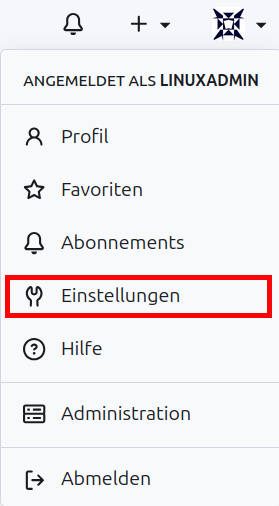
\includegraphics{bilder/inst/key1.png}
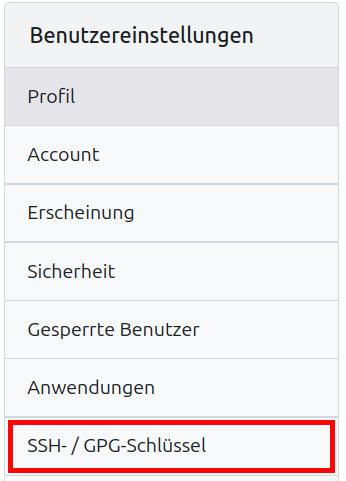
\includegraphics{bilder/inst/key2.png}
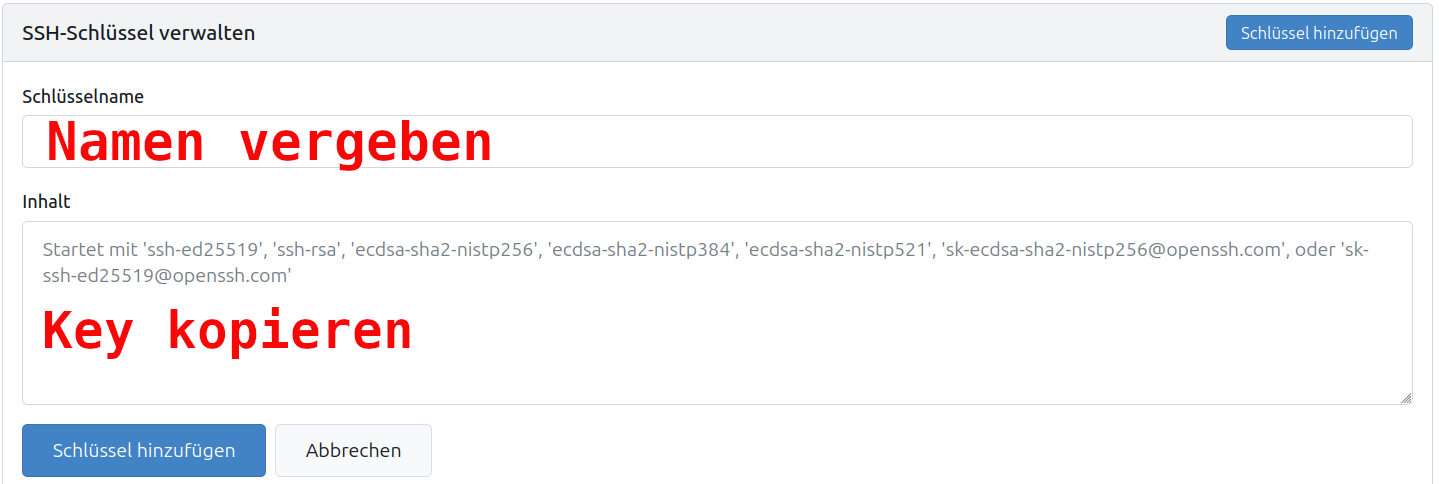
\includegraphics{bilder/inst/key3.png}

Damit ist die Grundkonfiguration beendet. Es sollte nun noch eingestellt
werden, welche Anmelde- und Registrierungsvarianten erlaubt sind, um
nicht plötzlich fremde Personen in seiner Gitea-Instanz zu haben.

\section{HTTPS}\label{https}

Aktuell ist die Instanz nur über \texttt{http} und Ip-Adresse
zugänglich. Es ist möglich, Gitea auch für \texttt{HTTPS} zu
konfigurieren. Hierfür gibt es verschiedenen Lösungen, von denen aber
eigentlich nur der Einsatz eines Reverse-Proxy mit einem entsprechenden
Domain-Name sinnvoll ist. Eine derartige Konfiguration würde den Rahmen
dieses Workshops aber sprengen! Zur Erinnerung: Es ging um eine
möglichst einfache Installation eines funktionsfähigen Systems.

\section{API}\label{api}

Oft ist es effizienter, wenn Dinge über Kommandozeile erledigt werden.
Wenn z.B. 50 Benutzerkonten erstellt und mit Passwort abgesichert werden
sollen, weil die Selbstregistrierung nicht gewünscht ist. In diese Fall
verwendet man die API von Gitea. Dies kann von jedem Rechner aus
erfolgen, auf Gitea zugreifen kann. Dafür braucht es aber noch zwei
Anpassungen an der \texttt{/etc/gitea/app.ini}:

\begin{enumerate}
\def\labelenumi{\arabic{enumi}.}
\tightlist
\item
  Ergänzen Sie am Ende der Datei:
\end{enumerate}

\begin{Shaded}
\begin{Highlighting}[]
\ExtensionTok{[api]}
\ExtensionTok{ENABLE\_ADMIN}\NormalTok{ = true}
\end{Highlighting}
\end{Shaded}

\begin{enumerate}
\def\labelenumi{\arabic{enumi}.}
\setcounter{enumi}{1}
\tightlist
\item
  Erweitern Sie den Abschnitt \texttt{security} falls Sie die Accounts
  mit sehr einfachen Kennwörtern vorbelegen wollen:
\end{enumerate}

\begin{Shaded}
\begin{Highlighting}[]
\ExtensionTok{[security]}
\ExtensionTok{...}\NormalTok{ bisheriger Inhalt ...}
\ExtensionTok{PASSWORD\_COMPLEXITY}\NormalTok{ = off}
\ExtensionTok{MIN\_PASSWORD\_LENGTH}\NormalTok{ = 6}
\end{Highlighting}
\end{Shaded}

Melden Sie sich als Administrator in Gitea an und rufen Sie das Menu
\emph{Einstellungen} des Benutzers auf. Unter \emph{Anwendungen} können
\emph{Admin-Token} erzeugt werden, die einen kennwortlosen Zugriff auf
das System erlauben. Stellen Sie im aufklappbaren Detail-Abschnitt ein,
welche Berechtigungen erforderlich sind:

\begin{itemize}
\tightlist
\item
  Admin - Lesen und Schreiben
\item
  Organisation
\item
  Repository
\item
  User
\end{itemize}

Kopieren Sie die lange Zahl (=Token) dann weg -- sie wird nur einmal
angezeigt!

Auf der Konsole (Linux / MacOS) kann dann z.B. folgender Befehl
abgeschickt werden, der die Benutzerin Susi anlegt:

\begin{Shaded}
\begin{Highlighting}[]
\ExtensionTok{curl} \AttributeTok{{-}X}\NormalTok{ POST }\StringTok{"http://\textless{}ip{-}adresse\textgreater{}:3000/api/v1/admin/users"} \DataTypeTok{\textbackslash{}}
\NormalTok{{-}H }\StringTok{"Authorization: token \textless{}kopiertes Token\textgreater{}"} \DataTypeTok{\textbackslash{}}
\NormalTok{{-}H }\StringTok{"Content{-}Type: application/json"} \DataTypeTok{\textbackslash{}}
\NormalTok{{-}d }\StringTok{\textquotesingle{}\{}
\StringTok{  "username": "susi",}
\StringTok{  "email": "susi@sandmann.com",}
\StringTok{  "password": "lalelu",}
\StringTok{  "send\_notify": false,}
\StringTok{  "must\_change\_password": true}
\StringTok{\}\textquotesingle{}}
\end{Highlighting}
\end{Shaded}

Verfeinert wird dieser Befehl in ein Script verpackt -- z.B.
\texttt{gitea\_user\_anlegen.sh}, das man mit einer Namensdatei als
Parameter aufrufen kann, in der folgende Spalten auftreten:

\begin{Shaded}
\begin{Highlighting}[]
\CommentTok{\# login,kennwort,email  \textless{}{-} Diese Zeile entfernen}
\ExtensionTok{susi,lalelu,susi@sandmann.de}
\ExtensionTok{max,foobla,max@mustermann.de}
\ExtensionTok{...}
\end{Highlighting}
\end{Shaded}

\subsection{Sinnvolle Szenarien}\label{sinnvolle-szenarien}

\subsubsection{Organisationen}\label{organisationen}

Hier bin ich mir nicht sicher, ob das kein Overkill ist. Eine Arbeit
über Teams erscheint mir bei der Größe unserer Szenarien deutlich
geeigneter. Das Problem ist nämlich, dass man über die API einen
Benutzer nur löschen kann, wenn er in keiner Organistation mehr ist!

Es könnte sinnvoll sein, wenn sich die einzelnen Kollegen als
\emph{Organisationen} sehen. Dann müssen Schüler aber mehrfach ins
System eingetragen werden und das bereits bei den eMail-Adressen
Probleme.

Sinnvoller erscheint eine Namenskonvention beim Erstellen von Teams!

\textbf{Organisation erstellen}

\begin{Shaded}
\begin{Highlighting}[]
\VariableTok{token}\OperatorTok{=}\NormalTok{1234}
\VariableTok{name}\OperatorTok{=}\NormalTok{G10a}
\ExtensionTok{curl} \AttributeTok{{-}X}\NormalTok{ POST }\StringTok{"http://192.168.3.195:3000/api/v1/admin/organizations"} \DataTypeTok{\textbackslash{}}
\NormalTok{{-}H }\StringTok{"Authorization: token }\VariableTok{$\{token\}}\StringTok{"} \DataTypeTok{\textbackslash{}}
\NormalTok{{-}H }\StringTok{"Content{-}Type: application/json"} \DataTypeTok{\textbackslash{}}
\NormalTok{{-}d }\StringTok{\textquotesingle{}\{}
\StringTok{  "username": "$\{name\}",}
\StringTok{  "full\_name": "$\{name\}",}
\StringTok{  "description": "Organisation für die Schüler der Klasse $\{name\}",}
\StringTok{  "visibility": "private"}
\StringTok{\}\textquotesingle{}}
\end{Highlighting}
\end{Shaded}

\textbf{Benutzer hinzufügen}

\begin{Shaded}
\begin{Highlighting}[]
\VariableTok{token}\OperatorTok{=}\NormalTok{1234}
\VariableTok{name}\OperatorTok{=}\NormalTok{G10a}
\VariableTok{user}\OperatorTok{=}\NormalTok{susi}
\ExtensionTok{curl} \AttributeTok{{-}X}\NormalTok{ PUT }\StringTok{"http://192.168.3.195:3000/api/v1/orgs/}\VariableTok{$\{name\}}\StringTok{$/members/}\VariableTok{$\{user\}}\StringTok{"} \DataTypeTok{\textbackslash{}}
\NormalTok{{-}H }\StringTok{"Authorization: token }\VariableTok{$\{token\}}\StringTok{"}
\end{Highlighting}
\end{Shaded}

\textbf{User löschen}

\begin{Shaded}
\begin{Highlighting}[]
\VariableTok{token}\OperatorTok{=}\NormalTok{1234}
\VariableTok{user}\OperatorTok{=}\StringTok{"susi"}
\CommentTok{\# In welchen Organistaionen ist der User}
\ExtensionTok{curl} \AttributeTok{{-}X}\NormalTok{ GET }\StringTok{"http://192.168.3.195:3000/api/v1/users/}\VariableTok{$\{user\}}\StringTok{/orgs"} \DataTypeTok{\textbackslash{}}
    \AttributeTok{{-}H} \StringTok{"Authorization: token }\VariableTok{$\{token\}}\StringTok{"}

\CommentTok{\# Einzeln austragen, sonst ist er nicht löschbar}
\VariableTok{orga}\OperatorTok{=}\NormalTok{organization1}
\ExtensionTok{curl} \AttributeTok{{-}X}\NormalTok{ DELETE }\StringTok{"http://192.168.3.195:3000/api/v1/orgs/}\VariableTok{$\{orga\}}\StringTok{/members/}\VariableTok{$\{user\}}\StringTok{"} \DataTypeTok{\textbackslash{}}
\NormalTok{{-}H }\StringTok{"Authorization: token }\VariableTok{$\{token\}}\StringTok{"}

\CommentTok{\# Benutzer löschen }
\ExtensionTok{curl} \AttributeTok{{-}X}\NormalTok{ DELETE }\StringTok{"http://192.168.3.195:3000/api/v1/admin/users/}\VariableTok{$\{user\}}\StringTok{"} \DataTypeTok{\textbackslash{}}
\NormalTok{{-}H }\StringTok{"Authorization: token }\VariableTok{$\{token\}}\StringTok{"}
\end{Highlighting}
\end{Shaded}

\subsection{Teams}\label{teams}

Auch ein Team erfordert eine Organisation -- hier würde ich einfach die
Schule anlegen.

\textbf{Team erstellen}

\begin{Shaded}
\begin{Highlighting}[]
\VariableTok{schule}\OperatorTok{=}\StringTok{"GGP"}
\VariableTok{token}\OperatorTok{=}\NormalTok{1234}
\VariableTok{team}\OperatorTok{=}\NormalTok{G10a}
\ExtensionTok{curl} \AttributeTok{{-}X}\NormalTok{ POST }\StringTok{"http://192.168.3.195:3000/api/v1/orgs/}\VariableTok{$\{schule\}}\StringTok{/teams"} \DataTypeTok{\textbackslash{}}
\NormalTok{{-}H }\StringTok{"Authorization: token }\VariableTok{$\{token\}}\StringTok{"} \DataTypeTok{\textbackslash{}}
\NormalTok{{-}H }\StringTok{"Content{-}Type: application/json"} \DataTypeTok{\textbackslash{}}
\NormalTok{{-}d }\StringTok{\textquotesingle{}\{}
\StringTok{  "name": "$\{team\}",}
\StringTok{  "description": "Team für das erste Projekt",}
\StringTok{  "permission": "write"}
\StringTok{\}\textquotesingle{}}
\end{Highlighting}
\end{Shaded}

\textbf{Benutzer hinzufügen}

\begin{Shaded}
\begin{Highlighting}[]
\VariableTok{schule}\OperatorTok{=}\NormalTok{GGP}
\VariableTok{token}\OperatorTok{=}\NormalTok{1234}
\VariableTok{team}\OperatorTok{=}\NormalTok{G10a}
\VariableTok{user}\OperatorTok{=}\NormalTok{susi}
\ExtensionTok{curl} \AttributeTok{{-}X}\NormalTok{ PUT }\StringTok{"http://192.168.3.195:3000/api/v1/orgs/}\VariableTok{$\{schule\}}\StringTok{/teams/}\VariableTok{$\{team\}}\StringTok{/members/}\VariableTok{$\{user\}}\StringTok{"} \DataTypeTok{\textbackslash{}}
\NormalTok{{-}H }\StringTok{"Authorization: token YOUR\_ADMIN\_TOKEN"}
\end{Highlighting}
\end{Shaded}

TODO: GPT shgt Team\_id statt Team\_name!

\bookmarksetup{startatroot}

\chapter{Docker}\label{docker}

Docker ist eine besonders effiziente Art der Virtualisierung. Es ist
möglich, auf einem physikalischen Server viele virtuelle Server zu
erstellen, diese miteinander kommunizieren und daten austauschen zu
lassen und sie auch über das Internet zugänglich zu machen. Es ist also
kein Problem, mehrere eigenständige Datenbankserver parallel zu
betreiben und damit Übungssystem für Schüler bereit zu stellen. Wie groß
der Server dimensioniert sein muss, hängt dann wieder von den speziellen
Anforderungen ab (mit 6 Cores und 16 GB RAM geht schon einiges, aber
sicher nicht alles!)

\section{Idee}\label{idee}

Nachdem Docker auf dem Server installiert ist (s.u.), kann man sich
einfach ein Betriebssystem-Image aus dem Netz herunterladen und als
Container starten. Natürlich ist es eine Vertrauensfrage, welche Images
man verwendet. Es gibt allerdings \emph{offizielle} Images von Firmen
und Organisationen, denen man vertrauen kann:

\begin{Shaded}
\begin{Highlighting}[]
\ExtensionTok{docker}\NormalTok{ search gitlab}

\ExtensionTok{NAME}\NormalTok{                             DESCRIPTION    STARS     OFFICIAL}
\ExtensionTok{alpinelinux/gitlab}\NormalTok{               Alpine...      11        }
\ExtensionTok{okteto/gitlab}\NormalTok{                                   3         }
\ExtensionTok{gitlab/gitlab{-}runner}\NormalTok{             GitLab ...     960       }
\ExtensionTok{vulhub/gitlab}\NormalTok{                                   1         }
\ExtensionTok{gitlab/gitlab{-}ce}\NormalTok{                 GitLab...      4310      }
\ExtensionTok{gitlab/gitlab{-}runner{-}helper}\NormalTok{                     50        }
\ExtensionTok{gitlab/gitlab{-}ee}\NormalTok{                 GitLab ...     549   }
\end{Highlighting}
\end{Shaded}

In dieser gekürzten Ausgabe ist also anscheinend kein \emph{offizielles}
Image dabei. \texttt{gitlab/gitlab-ce} ist aber trotzdem offiziell.
Dafür recherchiert man kurz auf \href{https://dockerhub.com}{dockerhub}
und dort ist \href{https://hub.docker.com/r/gitlab/gitlab-ce}{gitlab}
verlinkt, wo die Informationen stehen.

Wir werden übrigens nicht \emph{gitlab} sondern \emph{gitea} verwenden!

Von einem Image kann man dann beliebig viele Instanzen erzeugen, die
auch fast ohne Zeitverlust startbar sind. Der längste Teil ist der
Download des Image.

\textbf{Hintergrund}\\
Images sind in Schichten konstruiert, die nacheinander heruntergeladen
werden. Diese Schichtenstruktur ist wichtig, wenn man eigene Images
erstellen möchte. Der Erstellungsprozess macht nämlich immer auf der
Schicht weiter, ab der Änderungen am Image vorgenommen wurden (weitere
Software, Dateiänderungen, \ldots). Auf diese Weise wird viel weniger
Zeit benötigt, als bei einer komplett neuen Erstellung!

\section{Installation}\label{installation}

Die Befehle befinden sich auch bei den Kursmaterialien!

TODO - Docker install Script

\begin{Shaded}
\begin{Highlighting}[]
\FunctionTok{sudo} \AttributeTok{{-}i}
\ExtensionTok{apt}\NormalTok{ update}
\ExtensionTok{apt}\NormalTok{ install apt{-}transport{-}https curl }\AttributeTok{{-}y} 

\ExtensionTok{curl} \AttributeTok{{-}fsSL}\NormalTok{ https://download.docker.com/linux/ubuntu/gpg  }\DataTypeTok{\textbackslash{} }
     \KeywordTok{|} \ExtensionTok{gpg} \AttributeTok{{-}{-}dearmor} \AttributeTok{{-}o}\NormalTok{ /etc/apt/keyrings/docker.gpg}

\BuiltInTok{echo} \StringTok{"deb [arch=}\VariableTok{$(}\ExtensionTok{dpkg} \AttributeTok{{-}{-}print{-}architecture}\VariableTok{)}\StringTok{ \textbackslash{} }
\StringTok{      signed{-}by=/etc/apt/keyrings/docker.gpg] \textbackslash{} }
\StringTok{      https://download.docker.com/linux/ubuntu \textbackslash{} }
\StringTok{      }\VariableTok{$(}\BuiltInTok{.}\NormalTok{ /etc/os{-}release }\KeywordTok{\&\&} \BuiltInTok{echo} \StringTok{"}\VariableTok{$VERSION\_CODENAME}\StringTok{"}\VariableTok{)}\StringTok{ \textbackslash{} }
\StringTok{      stable"} \KeywordTok{|} \FunctionTok{tee}\NormalTok{ /etc/apt/sources.list.d/docker.list }\OperatorTok{\textgreater{}}\NormalTok{ /dev/null}

\ExtensionTok{apt}\NormalTok{ update}

\ExtensionTok{apt}\NormalTok{ install docker{-}ce docker{-}ce{-}cli }\DataTypeTok{\textbackslash{} }
    \ExtensionTok{containerd.io}\NormalTok{ docker{-}buildx{-}plugin }\DataTypeTok{\textbackslash{} }
    \ExtensionTok{docker{-}compose{-}plugin} \AttributeTok{{-}y}


\VariableTok{compose\_url}\OperatorTok{=}\StringTok{"https://github.com/docker/compose/releases/download"}
\ExtensionTok{curl} \AttributeTok{{-}L}  \VariableTok{$compose\_url}\NormalTok{/1.28.5/docker{-}compose{-}}\KeywordTok{\textasciigrave{}}\FunctionTok{uname} \DataTypeTok{\textbackslash{} }
     \ExtensionTok{{-}s}\KeywordTok{\textasciigrave{}}\AttributeTok{{-}}\KeywordTok{\textasciigrave{}}\FunctionTok{uname} \AttributeTok{{-}m}\KeywordTok{\textasciigrave{}} \AttributeTok{{-}o}\NormalTok{ /usr/local/bin/docker{-}compose}

\FunctionTok{chmod}\NormalTok{ +x /usr/local/bin/docker{-}compose}
\end{Highlighting}
\end{Shaded}

Aktuell läuft Docker jetzt als Benutzer \emph{root} (=Administrator),
was man im professionellen Firmenumfeld lieber vermeidet. Es gibt
Anleitung, wie man das ändert -- ich selbst verwende es aber auch so.

Teste die Installation durch folgende Befehle:

\begin{Shaded}
\begin{Highlighting}[]
\ExtensionTok{docker} \AttributeTok{{-}{-}version}
\ExtensionTok{docker{-}compose} \AttributeTok{{-}{-}version}
\end{Highlighting}
\end{Shaded}

\section{Kurzeinführung}\label{kurzeinfuxfchrung}

Es gibt sehr viele verschiedene Szenarien, wie Docker verwendet werden
kann und entsprechend sind auch die Befehle zahlreich und
unterschiedlich kompliziert.

Nachfolgend ein kleines \emph{Work-along}, wo einige Befehle verwendet
und erklärt werden. Tipp einfach mal folgenden Befehl:

\begin{Shaded}
\begin{Highlighting}[]
\ExtensionTok{docker}\NormalTok{ run }\AttributeTok{{-}d} \AttributeTok{{-}p}\NormalTok{ 8090:80 }\AttributeTok{{-}{-}name}\NormalTok{ it{-}tools corentinth/it{-}tools}
\end{Highlighting}
\end{Shaded}

Die Ausgabe (außer die Hashes) sollte dann so aussehen:

\begin{Shaded}
\begin{Highlighting}[]
\ExtensionTok{Unable}\NormalTok{ to find image }\StringTok{\textquotesingle{}corentinth/it{-}tools:latest\textquotesingle{}}\NormalTok{ locally}
\ExtensionTok{latest:}\NormalTok{ Pulling from corentinth/it{-}tools}
\ExtensionTok{43c4264eed91:}\NormalTok{ Pull complete }
\ExtensionTok{45a30f47e80f:}\NormalTok{ Pull complete }
\ExtensionTok{4c64d3291c88:}\NormalTok{ Pull complete }
\ExtensionTok{9dc0279166b1:}\NormalTok{ Pull complete }
\ExtensionTok{d3b17590914c:}\NormalTok{ Pull complete }
\ExtensionTok{50d6cfdb81c6:}\NormalTok{ Pull complete }
\ExtensionTok{6592d833752c:}\NormalTok{ Pull complete }
\ExtensionTok{f4cab7bcfad1:}\NormalTok{ Pull complete }
\ExtensionTok{65e7766bfa53:}\NormalTok{ Pull complete }
\ExtensionTok{c5f5268086b8:}\NormalTok{ Pull complete }
\ExtensionTok{Digest:}\NormalTok{ sha256:8b8128748339583ca951af03dfe02a9a4d7363f61a216226fc28030731a5a61f}
\ExtensionTok{Status:}\NormalTok{ Downloaded newer image for corentinth/it{-}tools:latest}
\ExtensionTok{bd072e349cab6408a3b5f2d7040d586a9149107d68031089f846d0526c028f45}
\end{Highlighting}
\end{Shaded}

Sieht nicht spktakulär aus, bis man \texttt{http://SERVERADRESSE:8090}
aufruft. Du hast hier einen kompletten Server voll mit digitalem
Spielzeug erstellt - in no time!

Natürlich kannst du den Container einfach weiter laufen lassen -- wir
wollen uns aber einige Dinge ansehen:

\begin{longtable}[]{@{}ll@{}}
\toprule\noalign{}
Befehl & Wirkung \\
\midrule\noalign{}
\endhead
\bottomrule\noalign{}
\endlastfoot
docker run & versucht einen Container zu erstellen \\
-d & im Hintergrund \\
-p 8090:80 & Von außen 8090, im Container eigentlich Port 80 \\
--name & sehen wir gleich \\
corentinth/it-tools & Name des Images \\
\end{longtable}

Es gibt nun zwei Stellen (oberflächlich) mit Informationen zu diesem
Server.

\begin{Shaded}
\begin{Highlighting}[]
\ExtensionTok{docker}\NormalTok{ image ls}
\end{Highlighting}
\end{Shaded}

Zeigt uns das heruntergeladene Image:

\begin{Shaded}
\begin{Highlighting}[]
\ExtensionTok{REPOSITORY}\NormalTok{             TAG       IMAGE ID       CREATED        SIZE}
\ExtensionTok{corentinth/it{-}tools}\NormalTok{    latest    bb7ba9626731   2 months ago   56.2MB}
\end{Highlighting}
\end{Shaded}

Mit nachfolgendem Befehl überprüft man den Status des Containers:

\begin{Shaded}
\begin{Highlighting}[]
\ExtensionTok{docker}\NormalTok{ ps }
\end{Highlighting}
\end{Shaded}

Ausgabe (gekürzt)

\begin{Shaded}
\begin{Highlighting}[]
\ExtensionTok{CONTAINER}\NormalTok{ ID   IMAGE                 COMMAND                  gekürzt ... NAMES }
\ExtensionTok{bd072e349cab}\NormalTok{   corentinth/it{-}tools   }\StringTok{"/docker{-}entrypoint.…"}\NormalTok{   gekürzt ... it{-}tools}
\end{Highlighting}
\end{Shaded}

\textbf{Weitere Befehle}\\
\textbar Befehl\textbar Wirkung\textbar{}
\textbar------\textbar-------\textbar{} \textbar docker stop
it-tools\textbar{} Container stoppen\textbar{} \textbar docker stop
bd072e349cab\textbar{} geht auch\textbar{} \textbar docker start
it-tools\textbar Container starten\textbar{} \textbar docker start
bd072e349cab\textbar{} geht auch\textbar{} \textbar docker rm
it-tools\textbar Container entfernen -- Image bleibt!\textbar{}
\textbar docker rmi ``corentinth/it-tools''\textbar Entfernt auch das
Image\textbar{}

Damit ein Container gelöscht werden kann, muss er beendet sein, damit
ein Image gelöscht werden kann, muss der Container gelöscht sein.

\section{Detaillierter}\label{detaillierter}

Für komplexere Szenarien wird der \emph{docker run} Befehl aber etwas
unübersichtlich. Man kann nun in zwei Stufen die Komplexität erhöhen:

\begin{itemize}
\tightlist
\item
  Anlegen einer Datei \emph{Dockerfile}, in der die Parameter für
  \emph{docker run} stehen
\item
  Verwenden von \emph{docker-compose} mit einer zusätzlichen Datei
  \emph{docker-compose.yml} um z.B. mehrere Server im Verbund zu
  managen. Dieses Verfahren werden wir bei der abschließenden,
  vollständigen Installation von Gitea verwenden.
\end{itemize}

Da sowohl Syntax als auch Varianten von beiden Stufen für eine schnelle
Behandlung zu komplex sind, verweise ich auf entsprechende Tutorial auf
youtube oder eines der vielen Bücher zum Thema -- z.B. von Michale
Kofler.

\bookmarksetup{startatroot}

\chapter{Gitea mit Docker}\label{gitea-mit-docker}

\section{Basics}\label{basics}

Wie im letzten Kapitel besprochen, wird der Einsatz von Docker durch
vorgefertigte Dockerfiles und Composefiles sehr vereinfacht. Erstellt
man selbst derartige Dateien, so sollte man Chatgpt nur sehr bedingt
vertrauen. In seinen Kreationen tauchen oft Konfigurationsparameter auf,
die es entweder gar nicht gibt, oder deren Schreibweise falsch ist.
Letztendlich führt kein Weg an der Herstellerdokumentation vorbei. Die
Dockerimages im Netz funktionieren aber gut, so dass man keine eigenen
bauen muss.

Bei einer vollwertigen Gitea-Installation brauchen wir (mindestens) drei
Container:

\begin{itemize}
\tightlist
\item
  Gitea
\item
  Datenbankserver
\item
  Runner (Erklärung folgt)
\end{itemize}

Mit dem nachfolgenden \texttt{docker-compose.yaml} können diese erstellt
und konfiguriert werden.

\textbf{Was ist ein Runner?}\\
In fortgeschrittenen Szenarien kann Gitea so konfiguriert werden, dass
ein Push auf einen bestimmten Branch zu nachgelagerten Aktionen auf dem
Server führt. Das können Unittests sein, aber auch Compilierungen,
Erstellung von Internetseiten, \ldots{} was mit dem versionierten Code
schlussendlich geplant ist. Wir werden unser Buch-Projekt so anpassen,
dass aus unseren Dokumenten automatisch ein druckreifes PDF erstellt
wird. Hier sind wir dann also bei der ursprünglichen Bedeutung der
\emph{Online-Kollaboration} angelangt.

Damit diese nachgelagerten Aktionen gestartet werden können, läuft eine
\emph{Runner}-Programm in einem eigenen Container. Dieses Programm
kommuniziert mit dem Gitea-Container und führt bei Bedarf die
entprechende Aktion aus. In eigentlich fast allen Fällen wird zum
Ausführen ein weiterer Docker-Container erstellt, der für die
eigentliche Aktion zuständig ist. Die Details dazu folgen weiter unten.

\section{Die Dateien}\label{die-dateien}

Natürlich kann man für jeden benötigten Container eine eigene
\texttt{docker-compose.yaml} erstellen, es ist aber sinnvoll, alle drei
Container gemeinsam zu konfigurieren, da dann auch Abhängigkeiten
zwischen den Containern autmatisch berücksichtigt werden. Wir besprechen
die verwendete \texttt{docker-compose.yaml} zuerst Zeile für Zeile. Die
vollständige Version steht am Ende des Kapitels und ist Teil der
Kursmaterialien.

\subsection{Allgemeine Einstellungen}\label{allgemeine-einstellungen}

\phantomsection\label{annotated-cell-142}%
\begin{Shaded}
\begin{Highlighting}[]
\FunctionTok{version}\KeywordTok{:}\AttributeTok{ }\StringTok{"3"}

\FunctionTok{networks}\KeywordTok{:}\CommentTok{ }\hspace*{\fill}\NormalTok{\circled{1}}
\AttributeTok{  }\FunctionTok{gitea}\KeywordTok{:}
\AttributeTok{    }\FunctionTok{external}\KeywordTok{:}\AttributeTok{ }\CharTok{true}\CommentTok{ }\hspace*{\fill}\NormalTok{\circled{2}}

\FunctionTok{volumes}\KeywordTok{:}\CommentTok{ }\hspace*{\fill}\NormalTok{\circled{3}}
\AttributeTok{  }\FunctionTok{gitea\_data}\KeywordTok{:}
\AttributeTok{    }\FunctionTok{driver}\KeywordTok{:}\AttributeTok{ local}
\AttributeTok{  }\FunctionTok{gitea\_db\_data}\KeywordTok{:}
\AttributeTok{    }\FunctionTok{driver}\KeywordTok{:}\AttributeTok{ local}
\AttributeTok{  }\FunctionTok{gitea\_runner\_data}\KeywordTok{:}
\AttributeTok{    }\FunctionTok{driver}\KeywordTok{:}\AttributeTok{ local}
\end{Highlighting}
\end{Shaded}

\begin{description}
\tightlist
\item[\circled{1}]
Alle drei Container müssen miteinander kommunizieren und werden deshalb
in ein gemeinsames Netz mit dem Namen \emph{gitea} eingebunden.
\item[\circled{2}]
Der Basis-Setup funktioniert hier auch mit \texttt{false}. Sobald der
Runner aber einen neuen Container erstellt, klappt das nur noch mit
\texttt{true}.
\item[\circled{3}]
Die Daten der Benutzer und die Einstellungen sollen auch über Neustarts
und Upgrades hinweg erhalten bleiben. Dafür dürfen sie nicht Teil des
Containers sein, der dabei komplett neu erstellt wird. Es werden auf
diese Weise drei Ordner mit den angegebenen Namen erstellt, die
außerhalb des Containers liegen und in diesen hinein verlinkt werden.
\end{description}

ToDo: Was hat es genau mit dem exteral:false auf sich? ToDo: Welche
andere Driver haben Volumens noch?

\subsection{Services}\label{services}

\begin{Shaded}
\begin{Highlighting}[]
\FunctionTok{services}\KeywordTok{:}
\AttributeTok{  }\FunctionTok{server}\KeywordTok{:}
\AttributeTok{    ...}
\AttributeTok{  }\FunctionTok{db}\KeywordTok{:}
\AttributeTok{    ...}
\AttributeTok{  }\FunctionTok{runner}\KeywordTok{:}
\AttributeTok{    ...}
\end{Highlighting}
\end{Shaded}

Dieser schematische Aufbau beschreibt die drei anzulegenden Container.
Wir besprechen die einzelnen Abschnitte nachfolgend getrennt.

\subsection{Server}\label{server}

\textbf{Teil 1}

\phantomsection\label{annotated-cell-144}%
\begin{Shaded}
\begin{Highlighting}[]
\AttributeTok{  }\FunctionTok{server}\KeywordTok{:}
\AttributeTok{    }\FunctionTok{image}\KeywordTok{:}\AttributeTok{ docker.io/gitea/gitea:1.22.6}\CommentTok{ }\hspace*{\fill}\NormalTok{\circled{1}}
\AttributeTok{    }\FunctionTok{container\_name}\KeywordTok{:}\AttributeTok{ gitea}
\AttributeTok{    }\FunctionTok{hostname}\KeywordTok{:}\AttributeTok{ gitea}
\AttributeTok{    }\FunctionTok{environment}\KeywordTok{:}
\AttributeTok{      }\KeywordTok{{-}}\AttributeTok{ USER\_UID=1000}
\AttributeTok{      }\KeywordTok{{-}}\AttributeTok{ USER\_GID=1000}
\AttributeTok{      }\KeywordTok{{-}}\AttributeTok{ GITEA\_\_database\_\_DB\_TYPE=mysql}\CommentTok{ }\hspace*{\fill}\NormalTok{\circled{2}}
\AttributeTok{      }\KeywordTok{{-}}\AttributeTok{ GITEA\_\_database\_\_HOST=db:3306}\CommentTok{ }\hspace*{\fill}\NormalTok{\circled{3}}
\AttributeTok{      }\KeywordTok{{-}}\AttributeTok{ GITEA\_\_database\_\_NAME=gitea}\CommentTok{ }\hspace*{\fill}\NormalTok{\circled{4}}
\AttributeTok{      }\KeywordTok{{-}}\AttributeTok{ GITEA\_\_database\_\_USER=gitea}
\AttributeTok{      }\KeywordTok{{-}}\AttributeTok{ GITEA\_\_database\_\_PASSWD=gitea}
\end{Highlighting}
\end{Shaded}

\begin{description}
\tightlist
\item[\circled{1}]
Hier könnte auch \texttt{gitea:latest} stehen, was Upgrades vereinfacht.
\item[\circled{2}]
Möglich sind auch \emph{postgresql} und \emph{sqlite}. Sqlite ist eine
Alternative für kleine Installationen, da dabei kein eigener
Datenbankserver benötigt wird.
\item[\circled{3}]
Name des Datenbankservers:Port
\item[\circled{4}]
Hochsicherheitskennwörter für die Fortbildung
\end{description}

\textbf{Teil 2}

\phantomsection\label{annotated-cell-145}%
\begin{Shaded}
\begin{Highlighting}[]
\AttributeTok{    }\FunctionTok{restart}\KeywordTok{:}\AttributeTok{ always}\CommentTok{ }\hspace*{\fill}\NormalTok{\circled{1}}
\AttributeTok{    }\FunctionTok{networks}\KeywordTok{:}\CommentTok{ }\hspace*{\fill}\NormalTok{\circled{2}}
\AttributeTok{      }\KeywordTok{{-}}\AttributeTok{ gitea}
\AttributeTok{    }\FunctionTok{volumes}\KeywordTok{:}\CommentTok{ }\hspace*{\fill}\NormalTok{\circled{3}}
\AttributeTok{      }\KeywordTok{{-}}\AttributeTok{ gitea\_data:/data}
\AttributeTok{      }\KeywordTok{{-}}\AttributeTok{ /etc/timezone:/etc/timezone:ro}
\AttributeTok{      }\KeywordTok{{-}}\AttributeTok{ /etc/localtime:/etc/localtime:ro}
\AttributeTok{    }\FunctionTok{ports}\KeywordTok{:}
\AttributeTok{      }\KeywordTok{{-}}\AttributeTok{ }\StringTok{"4000:3000"}\CommentTok{ }\hspace*{\fill}\NormalTok{\circled{4}}
\AttributeTok{      }\KeywordTok{{-}}\AttributeTok{ }\StringTok{"222:22"}\CommentTok{ }\hspace*{\fill}\NormalTok{\circled{5}}
\AttributeTok{    }\FunctionTok{depends\_on}\KeywordTok{:}\CommentTok{ }\hspace*{\fill}\NormalTok{\circled{6}}
\AttributeTok{      }\KeywordTok{{-}}\AttributeTok{ db}
\end{Highlighting}
\end{Shaded}

\begin{description}
\tightlist
\item[\circled{1}]
Container immer automatisch neu starten, wenn etwas schief geht oder der
Server neu gestartet wird.
\item[\circled{2}]
Festlegen des Netzes in dem der Container läuft
\item[\circled{3}]
Die Daten von Gitea liegen im Ordner \texttt{gitea\_data}, genauer unter
\texttt{/var/lib/docker/volumes/gitea\_data}. Über Volumes wird aber
auch der Zugriff auf Ressourcen des Servers gesteuert, hier der Zugriff
die Eistellungen der Zeitzone. (\texttt{:ro} nur lesender Zugriff)
\item[\circled{4}]
IM Container läuft Gitea auf Port 3000, der Zugriff von außen (Browser)
erfolgt über Port 4000. Ist hier eher als Demo gedacht, 3000:3000 ginge
auch.
\item[\circled{5}]
Der SSH-Server (für pull, push, \ldots) läuft im Container auf Port 22,
Zugriff von außen über Port 222. Das ist nötig, da der Server (also der
gemietete Server) seinen ssh-Server bereits auf Port 22 laufen hat. Das
kann man zwar ändern, muss aber etwas aufpassen, dass man sich nit
versehentlich aussperrt, weil man die Firewall nicht angepasst hat.
\item[\circled{6}]
Der Container wird erst gestartet, wenn der Datenbankserver erfolgreich
hochgefahren ist.
\end{description}

\subsection{db}\label{db}

Alle relevanten Zeilen sind analog zum obigen Beispiel zu lesen.

\begin{Shaded}
\begin{Highlighting}[]
\AttributeTok{  }\FunctionTok{db}\KeywordTok{:}
\AttributeTok{    }\FunctionTok{image}\KeywordTok{:}\AttributeTok{ docker.io/library/mysql:8}
\AttributeTok{    }\FunctionTok{restart}\KeywordTok{:}\AttributeTok{ always}
\AttributeTok{    }\FunctionTok{container\_name}\KeywordTok{:}\AttributeTok{ db}
\AttributeTok{    }\FunctionTok{hostname}\KeywordTok{:}\AttributeTok{ db}
\AttributeTok{    }\FunctionTok{environment}\KeywordTok{:}
\AttributeTok{      }\KeywordTok{{-}}\AttributeTok{ MYSQL\_ROOT\_PASSWORD=gitea}
\AttributeTok{      }\KeywordTok{{-}}\AttributeTok{ MYSQL\_USER=gitea}
\AttributeTok{      }\KeywordTok{{-}}\AttributeTok{ MYSQL\_PASSWORD=gitea}
\AttributeTok{      }\KeywordTok{{-}}\AttributeTok{ MYSQL\_DATABASE=gitea}
\AttributeTok{    }\FunctionTok{networks}\KeywordTok{:}
\AttributeTok{      }\KeywordTok{{-}}\AttributeTok{ gitea}
\AttributeTok{    }\FunctionTok{volumes}\KeywordTok{:}
\AttributeTok{      }\KeywordTok{{-}}\AttributeTok{ gitea\_db\_data:/var/lib/mysql}
\end{Highlighting}
\end{Shaded}

\subsection{runner}\label{runner}

Es werden hier nur neue oder wichtige Einstellungen erklärt!

\phantomsection\label{annotated-cell-147}%
\begin{Shaded}
\begin{Highlighting}[]
\AttributeTok{  }\FunctionTok{runner}\KeywordTok{:}
\AttributeTok{    }\FunctionTok{image}\KeywordTok{:}\AttributeTok{ docker.io/gitea/act\_runner:latest}
\AttributeTok{    }\FunctionTok{container\_name}\KeywordTok{:}\AttributeTok{ gitea\_runner}
\AttributeTok{    }\FunctionTok{hostname}\KeywordTok{:}\AttributeTok{ gitea\_runner}
\AttributeTok{    }\FunctionTok{environment}\KeywordTok{:}
\AttributeTok{      }\FunctionTok{CONFIG\_FILE}\KeywordTok{:}\AttributeTok{ /config.yaml}\CommentTok{ }\hspace*{\fill}\NormalTok{\circled{1}}
\AttributeTok{      }\FunctionTok{GITEA\_INSTANCE\_URL}\KeywordTok{:}\AttributeTok{ }\StringTok{"http://gitea:3000"}
\AttributeTok{      }\FunctionTok{GITEA\_RUNNER\_NAME}\KeywordTok{:}\AttributeTok{ }\StringTok{"Probe{-}runner"}
\AttributeTok{      }\FunctionTok{GITEA\_RUNNER\_REGISTRATION\_TOKEN}\KeywordTok{:}\AttributeTok{ \textless{}ausfüllen\textgreater{}}\CommentTok{ }\hspace*{\fill}\NormalTok{\circled{2}}
\AttributeTok{    }\FunctionTok{restart}\KeywordTok{:}\AttributeTok{ always}
\AttributeTok{    }\FunctionTok{depends\_on}\KeywordTok{:}\CommentTok{ }\hspace*{\fill}\NormalTok{\circled{3}}
\AttributeTok{      }\KeywordTok{{-}}\AttributeTok{ server}
\AttributeTok{      }\KeywordTok{{-}}\AttributeTok{ db}
\AttributeTok{    }\FunctionTok{networks}\KeywordTok{:}
\AttributeTok{      }\KeywordTok{{-}}\AttributeTok{ gitea}
\AttributeTok{    }\FunctionTok{volumes}\KeywordTok{:}
\AttributeTok{      }\KeywordTok{{-}}\AttributeTok{ ./config.yaml:/config.yaml}\CommentTok{ }\hspace*{\fill}\NormalTok{\circled{4}}
\AttributeTok{      }\KeywordTok{{-}}\AttributeTok{ gitea\_runner\_data:/data}
\AttributeTok{      }\KeywordTok{{-}}\AttributeTok{ /etc/timezone:/etc/timezone:ro}
\AttributeTok{      }\KeywordTok{{-}}\AttributeTok{ /etc/localtime:/etc/localtime:ro}
\AttributeTok{      }\KeywordTok{{-}}\AttributeTok{ /var/run/docker.sock:/var/run/docker.sock}\CommentTok{ }\hspace*{\fill}\NormalTok{\circled{5}}
\end{Highlighting}
\end{Shaded}

\begin{description}
\tightlist
\item[\circled{1}]
Dazu kommt unten mehr!
\item[\circled{2}]
Füllen wir später noch aus
\item[\circled{3}]
Dieser Container startet erst wenn die beiden anderen laufen
\item[\circled{4}]
Ein Volume kann auch nur eine einzige Datei sein. Beachte den
Unterschied bei der Schreibung von \texttt{./config.yaml} und
\texttt{gitea\_runner\_data}. Das \texttt{./} am Anfang bedeutet, dass
diese Datei im gleichen Ordner liegt wie die
\texttt{docker-compose.yaml}.
\item[\circled{5}]
Dieser Container braucht auch selbst Zugriff auf Docker, damit er selbst
neue Container starten kann.
\end{description}

\textbf{Das Config-File}\\
Bei vielen Containern kann die Konfiguration durch Einträge in der
\texttt{docker-compose.yaml} erfolgen - wie z.B. die Kennwörter. Gerade
für Kennwörter gibt es noch sicherere Varianten, das führt aber zu weit.
Für den Runner werden aber noch Einstellungen nötig, die man so
(anscheinend) nicht übergeben kann. Aus diesem Grund wird oben der
Parameter \texttt{CONFIG\_FILE} übergeben. Diese Datei befindet sich
ebenfalls in den Kursmaterialien und wird hier nicht abgedruckt. Für
eine frische Datei kann man folgenden Befehl aufrufen:

\begin{Shaded}
\begin{Highlighting}[]
\ExtensionTok{docker}\NormalTok{ exec }\AttributeTok{{-}it}\NormalTok{ gitea\_runner act\_runner generate{-}config}
\end{Highlighting}
\end{Shaded}

oder direkt als Datei

\begin{Shaded}
\begin{Highlighting}[]
\ExtensionTok{docker}\NormalTok{ exec }\AttributeTok{{-}it}\NormalTok{ gitea\_runner act\_runner generate{-}config }\OperatorTok{\textgreater{}}\NormalTok{ config.yaml}
\end{Highlighting}
\end{Shaded}

\samplestart

\textbf{Hinweis}\\
Vielleicht ist dir aufgafallen, dass einmal im Environment
Spiegelstriche vorkommen und einmal nicht. Das ist Absicht, denn die
Server wollen das unterschiedlich haben. Intern wird bei der
Spiegelstrich-Variante eine Liste der Art
\texttt{{[}"key=value",\ "key=vlaue",\ ...{]}\ erstellt,\ die\ der\ \ Server\ verarbeiten\ muss.\ Der\ Runner\ hätte\ aber\ lieber\ ein\ Dictionary,\ d.h.\ eine\ Darstellung}\{key:value,
key:value, \ldots\}` und das passiert \textbf{ohne} die Spiegelstriche.
\sampleend

\textbf{Das Registrierungs-Token}\\
Bist du in Gitea eingelogged, so kannst du über das Einstellungsmenü
(Das geht auf Instanz-, Repository- oder Userebene) nach \emph{actions}
suchen, dort auf \emph{runner} und dann oben rechts auf \emph{neuen
runner anlegen} (o.ä.). Dort erscheint dann das Token, das in die
\texttt{docker-compose.yaml} eingetragen werden muss. Beim Neustart
registriert sich der Runner dann damit bei Gitea.

\subsection{Starten}\label{starten}

Damit der Runner gestartet werden kann, muss zunächst Gitea laufen --
sonst kann man kein Token erstellen.

\begin{Shaded}
\begin{Highlighting}[]
\ExtensionTok{docker{-}compose}\NormalTok{ up gitea db }
\end{Highlighting}
\end{Shaded}

Später wird der Befehl mit einem zusätzlichen \texttt{-d} gestartet,
damit der Start im Hintergrund erfolgt. Ohne \texttt{-d} sieht man
eventuelle Fehlermeldungen.

Nun kannst du dich bei Gitea im Browser anmelden und den ersten Benutzer
einrichten, den du dann auch als Administrator verwenden kannst.

TODO: Anmeldescreen

Im Prinzip kann man auch Mailregistrierung und andere Dinge
konfigurieren -- für einen einfachen Betrieb genügt aber das Einrichten
des Benutzers.

Nach dem oben beschriebenen Erstellen eines Tokens kannst du den Gitea
und den DB-Server mit \texttt{ctrl-c} zunächst wieder beenden. Das Token
wird nun in die \texttt{docker-compose.yaml} kopiert.

Nun kann auch der Runner gestartet werden. Auch jetzt zu Testzwecken
zuerst ohne \texttt{-d}:

\begin{Shaded}
\begin{Highlighting}[]
\ExtensionTok{docker{-}compose}\NormalTok{ up}
\end{Highlighting}
\end{Shaded}

Hat das ohne Fehler geklappt, dann wieder \texttt{strg\ +\ c} und dann
ein richtiger Start:

\begin{Shaded}
\begin{Highlighting}[]
\ExtensionTok{docker{-}compose}\NormalTok{ up }\AttributeTok{{-}d}
\end{Highlighting}
\end{Shaded}

Gitea sollte jetzt verwendbar sein!

\subsection{Einrichten}\label{einrichten}

Im Prinzip ist Gitea bereits voll funktionsfähig. Wenn die Schüler
\textbf{nur} über den Browser mit dem System arbeiten, sind auch keine
weiteren Einstellungen nötig. Wird aber vollwertiger Zugriff
(clone/pull/push) benötigt, so müssen die Benutzer noch ihren
ssh-Schlüssel im System hinterlegen.

\subsection{Schlüssel erstellen}\label{schluxfcssel-erstellen}

\textbf{Auf Linux und MacOS}

\begin{Shaded}
\begin{Highlighting}[]
\FunctionTok{ssh{-}keygen} \AttributeTok{{-}t}\NormalTok{ rsa }\AttributeTok{{-}b}\NormalTok{ 4096 }
\end{Highlighting}
\end{Shaded}

Im weiteren Verlauf wird nach einer Keyphrase gefragt -- leer lassen --
und ein Name für den Schlüssel abgefragt -- gitea passt gut.

Diesen Schlüssel lässt man sich ausgeben:

\begin{Shaded}
\begin{Highlighting}[]
\FunctionTok{cat}\NormalTok{ \textasciitilde{}/.ssh/gitea.pub}
\end{Highlighting}
\end{Shaded}

In den Benutzereinstellungen auf Gitea kann nun ein neuer Schlüssel
hinzugefügt werden.

TODO: Eventuell Screenshot

\textbf{Auf Windows}\\
\ldots{} ach ja \ldots{} Windows \ldots{}

\subsection{Clonen}\label{clonen}

Das Clonen eines öffentlichen Repositories über Https sollte auch ohne
Schlüssel funktionieren. Für einen vollwertigen Zugriff verwendet man
aber lieber \emph{ssh} und zwar mit folgendem Befehl:

\begin{Shaded}
\begin{Highlighting}[]
\FunctionTok{git}\NormalTok{ clone ssh://git@mein\_server:222/BENUTZER/REPO.git}
\end{Highlighting}
\end{Shaded}

Die Angabe von 222 ist nötig, da wir nicht Port 22 verwenden -- man muss
also die Adresse, die man in Gitea über dem Repository sieht, noch
entsprechend anpassen.

TODO: Screenshot

\bookmarksetup{startatroot}

\chapter{Actions}\label{actions}

Dieses Thema ist nun so groß und speziell, dass wir an unsere Genzen
stoßen. Ich möchte nur kurz das Vorgehen für unser Szenario der
Bucherstellung besprechen.

\bookmarksetup{startatroot}

\chapter{Clients}\label{clients}

Generell gilt natürlich, dass im Informatikunterricht ein Tablet (oder
Handy) kein geeignetes Werkzeug ist. Wir sprechen im Folgenden also von
Laptops oder Desktops und diese können mit Windows, MacOS, Linux oder
ChromeOS ausgestattet sein. Für jedes dieser Systeme gibt es viele
verschiedene Git-Clients. Die Kommandozeile (Terminal, Bash, Git-Bash,
\ldots) ohne grafische Benutzeroberfläche ist gerade bei Anfängern nicht
besonders beliebt, aber gerade im Umfeld von Servern sehr verbreitet.
Entwickler, die mir den IDEs von JetBrains, VS-Code, o.ä. arbeiten,
verwenden oft die dort eingebauten Git-Clients. Leider sind diese
Entwicklungsumgebungen dür den Einsatz im Unterricht ein Overkill. Bei
einer kleineren IDE kann ein graphischer Git-Client diese Lücke
schließen.\\
Probleme gibt es allerdings traditionell bei der heimischen Installation
der entsprechenden Software (GitKraken, \ldots). Mit Hilfe von
\emph{portable} Versionen kann das aber deutlich vereinfacht werden.
Diese Software-Variante wird nicht installiert, sondern lediglich
entpackt. Der entstehende Ordner kann sogar auf einen USB-Stick
ausgelagert werden. Damit sind auch die Rechner der Eltern problemlos
benutzbar.

\href{https://git-scm.com/downloads/win}{Portable Git}

\bookmarksetup{startatroot}

\chapter{Autograding}\label{autograding}

Der Workflow für das Autograding von Schülerlösungen unterscheidet sich
deutlich von der normalen Arbeit mit git/gitea, weil man den
\emph{kreativen Wissenstransfer} doch möglichst vermeiden möchte.\\
Beim Autograding geht es im Prinzip darum, dass die Schüler ihre
Aufgaben / Prüfungen auf eine Art und Weise schreiben, dass sie mit
automatisierten Test überprüft werden können. Hierbei können sichtbare
Tests (der Schüler sieht sofort, ob seine Lösung passt) und versteckte
Tests verwendet werden.\\
Technisch gesehen führt der Schüler einen Commit aus, der die
Überprüfung triggert. Es ist auch möglich, dass sich der Lehrer die
Schülerlösungen holt und dann erst testet.

\section{Vorarbeiten}\label{vorarbeiten}

\begin{itemize}
\tightlist
\item
  Die Schüler müssen im System sein.
\item
  Erstellen eines Teams
\item
  Schüler dem Team zuordnen
\item
  Ein Repository für Hausaufgaben oder spezielle Prüfungen erstellen und
  die benötigten Materialien hinein kopieren.
\end{itemize}

Das Script aus den Kursmaterialien führt dann für alle Teammitglieder
nachfolgende Schritte aus * Das Repository für den Schüler
\emph{forken}, d.h. eine vollwertige Kopie erstellen * Die
Berechtigungen so setzen, dass kein Schüler den Fork eines Mitschülers
sehen kann

\section{Workflow Schüler}\label{workflow-schuxfcler}

Das hängt nun von der genauen Aubeitsweise ab. Im Prinzip muss der
Schüler die Aufgabenstellung in der Aufgabendatei erledigen, die im
Original-Repository erstellt wurde. Nach dem Erstellen der Lösung wird
die Arbeit committet und auf den Server gepusht. Dort greifen dann die
nachfolgende Automatismen.

Da das gleiche Repo (Hausaufgaben) über einen längeren Zeitraum genutzt
werden soll, muss der Schüler regelmäßig die Änderungen im Origina-Repo
in seinen Fork übertragen. Der Lehrer har dafür zu sorgen (Anleitung,
\ldots) dass es Dateien gibt (Namenskonvention), die der Schüler nicht
anfasst. Auf diese Weise werden Merge-Konflikte vermieden, wenn
Original-Repo und Fork zusammengeführt werden.

\begin{Shaded}
\begin{Highlighting}[]
\FunctionTok{git}\NormalTok{ pull }


\CommentTok{\#\# Ablauf}

\ExtensionTok{*}\NormalTok{ Schüler einrichten}
\ExtensionTok{*}\NormalTok{ CI/CD System einrichten }\AttributeTok{{-}}\NormalTok{ hier wird auf jenkins verweisen}\PreprocessorTok{?}\NormalTok{ Geht auch otter{-}grader}\PreprocessorTok{?}
\ExtensionTok{*}\NormalTok{ Vorlagen für verschiedene Aufgaben erstellen }\PreprocessorTok{?????}
\ExtensionTok{*}\NormalTok{ Anleitung durch README.md}


\CommentTok{\#\# Beginn des Kurses}

\ExtensionTok{*}\NormalTok{ Der Lehrer erstellt ein Repo}
\ExtensionTok{*}\NormalTok{ Die Schüler forken das über die GUI}
\ExtensionTok{*}\NormalTok{ Die Schüler Clonen ihr eigenes Repo}
\end{Highlighting}
\end{Shaded}

git clone https://gitea.example.com/student1/haupt-repository.git

\begin{verbatim}
* Jeden Tag wird das Repo gepullt
\end{verbatim}

cd haupt-repository git pull origin main

\begin{verbatim}
* Die Hausaufgaben werden committed und gepusht
```bash
git add . --all
git commit -m "erledigt"
\end{verbatim}

\begin{itemize}
\tightlist
\item
  Der Lehrer sammelt die Arbeien ein
\end{itemize}

\begin{Shaded}
\begin{Highlighting}[]
\CommentTok{\#!/bin/bash}

\VariableTok{STUDENT\_REPOS}\OperatorTok{=}\VariableTok{(}\StringTok{"https://gitea.example.com/student1/hausaufgaben.git"} \StringTok{"https://gitea.example.com/student2/hausaufgaben.git"}\VariableTok{)}
\VariableTok{LOCAL\_DIR}\OperatorTok{=}\StringTok{"student\_submissions"}

\FunctionTok{mkdir} \AttributeTok{{-}p} \VariableTok{$LOCAL\_DIR}
\BuiltInTok{cd} \VariableTok{$LOCAL\_DIR}

\ControlFlowTok{for}\NormalTok{ REPO }\KeywordTok{in} \StringTok{"}\VariableTok{$\{STUDENT\_REPOS}\OperatorTok{[@]}\VariableTok{\}}\StringTok{"}\KeywordTok{;} \ControlFlowTok{do}
  \VariableTok{REPO\_NAME}\OperatorTok{=}\VariableTok{$(}\FunctionTok{basename} \VariableTok{$REPO}\NormalTok{ .git}\VariableTok{)}
  \ControlFlowTok{if} \BuiltInTok{[} \OtherTok{{-}d} \StringTok{"}\VariableTok{$REPO\_NAME}\StringTok{"} \BuiltInTok{]}\KeywordTok{;} \ControlFlowTok{then}
    \BuiltInTok{cd} \VariableTok{$REPO\_NAME}
    \FunctionTok{git}\NormalTok{ pull origin main}
    \BuiltInTok{cd}\NormalTok{ ..}
  \ControlFlowTok{else}
    \FunctionTok{git}\NormalTok{ clone }\VariableTok{$REPO}
  \ControlFlowTok{fi}
\ControlFlowTok{done}
\end{Highlighting}
\end{Shaded}

\bookmarksetup{startatroot}

\chapter{Introduction}\label{introduction}

This is a book created from markdown and executable code.

See Knuth (1984) for additional discussion of literate programming.

\bookmarksetup{startatroot}

\chapter{Summary}\label{summary}

In summary, this book has no content whatsoever.

\bookmarksetup{startatroot}

\chapter*{References}\label{references}
\addcontentsline{toc}{chapter}{References}

\markboth{References}{References}

\phantomsection\label{refs}
\begin{CSLReferences}{1}{0}
\bibitem[\citeproctext]{ref-knuth84}
Knuth, Donald E. 1984. {„Literate Programming``}. \emph{Comput. J.} 27
(2): 97--111. \url{https://doi.org/10.1093/comjnl/27.2.97}.

\end{CSLReferences}




\end{document}
